%% Supplementary material for the ISPRS Journal of Photogrammetry and Remote
%% Sensing submission, converted from paper/supplement.md by
%% scripts/paper_to_elsevier.py. Upload its PDF as supplementary material.
%% References to the manuscript use its numbering (Section 4.1, Table 3).
\documentclass[10pt,a4paper]{article}
\usepackage[T1]{fontenc}
\usepackage{mathptmx}
\renewcommand{\ttdefault}{pcr}
\renewcommand{\sfdefault}{phv}
\usepackage[a4paper,margin=2cm]{geometry}
\usepackage[round,authoryear,sort]{natbib}
\usepackage{amsmath}
\usepackage{graphicx}
\ifdefined\pdfsuppresswarningpagegroup\pdfsuppresswarningpagegroup=1\relax\fi
\usepackage{array}
\usepackage{xltabular}
\usepackage{booktabs}
\usepackage{url}
\usepackage[hidelinks]{hyperref}
\providecommand{\tightlist}{\setlength{\itemsep}{0pt}\setlength{\parskip}{0pt}}
\newcolumntype{L}{>{\raggedright\arraybackslash}X}
\newcolumntype{R}{>{\raggedleft\arraybackslash}X}
\newcolumntype{C}{>{\centering\arraybackslash}X}
\graphicspath{{./}{../}}
\setlength{\parindent}{0pt}
\setlength{\parskip}{4pt}
\setlength{\emergencystretch}{3em}
\newcommand{\DOIprefix}{}
\newcommand{\URLprefix}{}
\newcommand{\doi}[1]{\url{https://doi.org/#1}}
\makeatletter
% Figures float ([!ht]), so the text of their section fills the page before
% them, but never leave their section: before each section the figures still
% waiting go to the top of the next page, and after a section's heading no
% figure goes above it on the same page (as in the IEEE supplement).
\newcommand\suppFloatBarrier{\par\addpenalty\z@
  \ifx\@deferlist\@empty\else\expandafter\supp@flush\fi}
\newcommand\supp@flush{\let\supp@waiting\@deferlist
  \newpage
  \ifx\@deferlist\supp@waiting\null\newpage\fi
  \ifx\@deferlist\supp@waiting\expandafter\clearpage\else\expandafter\suppFloatBarrier\fi}
\gdef\supp@afterheading{}
\g@addto@macro\@afterheading{\supp@afterheading}
\AtBeginDocument{\let\supp@section\section
  \renewcommand\section{\suppFloatBarrier
    \gdef\supp@afterheading{\suppressfloats[t]\gdef\supp@afterheading{}}\supp@section}}
\makeatother

\title{Supplementary material for ``Choosing tree detectors by point density:
a field-stem benchmark for national-mapping airborne LiDAR''}
% TODO: list every author here too, as in main.tex.
\author{Alexey Grigoryev}
\date{}

\begin{document}
\maketitle

Supplement to the manuscript ``Choosing tree detectors by point density: a field-stem benchmark for national-mapping airborne LiDAR.'' Each section names the study report its numbers come
from. Density is the median first-return pulse density inside the plot cores of
the 106 plots: 9.8 pulses/m\textsuperscript{2} at native density and 4.4, 2.2, 1.8, 1.1 and 0.6
pulses/m\textsuperscript{2} at the five decimated density levels (Section~S26). The level at 1.8
pulses/m\textsuperscript{2} was declared to stand at the QL2 floor of 2 pulses/m\textsuperscript{2} by its
whole-clip density and is called the QL2 level. Every LiDAR detector reads the
same fixed evaluation clips (Section~3.3 of the manuscript).

\section*{S1. Recall by crown class}

Native density, five sites, nominal plot core, with 95\% plot-bootstrap
intervals: 1,872 overstory stems (dominant and codominant) and 592 understory
stems (intermediate and suppressed), 404 of the latter at WREF. Detections carry
no crown class, so the strata have recall only. Source: \href{https://github.com/devakellc/lidar-tree-benchmark/blob/main/results/master-tables-results.md}{master
tables}.

{\footnotesize
\setlength{\tabcolsep}{3pt}
\renewcommand{\arraystretch}{1.15}
\begin{xltabular}{\textwidth}{lLL}
\multicolumn{3}{@{}p{\textwidth}@{}}{\normalsize\textbf{Table S1.} Recall by crown class at native density.} \\[4pt]
\toprule
Detector & Overstory & Understory \\
\midrule
\endfirsthead
\multicolumn{3}{@{}l@{}}{\normalsize\textbf{Table S1} (continued)} \\[4pt]
\toprule
Detector & Overstory & Understory \\
\midrule
\endhead
\bottomrule
\endfoot
AMS3D & 0.735 [0.686, 0.777] & 0.627 [0.560, 0.701] \\
\texttt{ptrees} & 0.786 [0.746, 0.827] & 0.459 [0.365, 0.555] \\
ForestFormer3D & 0.674 [0.645, 0.704] & 0.454 [0.387, 0.522] \\
\texttt{multichm} & 0.599 [0.568, 0.632] & 0.340 [0.291, 0.396] \\
SegmentAnyTree & 0.698 [0.657, 0.739] & 0.291 [0.218, 0.364] \\
DeepForest (RGB) & 0.630 [0.594, 0.667] & 0.262 [0.206, 0.323] \\
Li 2012 & 0.663 [0.617, 0.710] & 0.228 [0.159, 0.298] \\
\texttt{lmfauto} & 0.658 [0.605, 0.708] & 0.225 [0.149, 0.300] \\
TreeisoNet & 0.606 [0.562, 0.650] & 0.193 [0.131, 0.256] \\
CHM-VWF & 0.554 [0.511, 0.601] & 0.171 [0.118, 0.226] \\
Detectree2 (RGB) & 0.365 [0.325, 0.403] & 0.123 [0.089, 0.162] \\
\end{xltabular}
}

\section*{S2. Accuracy by site}

Source: \href{https://github.com/devakellc/lidar-tree-benchmark/blob/main/results/master-tables-results.md}{master tables} and \href{https://github.com/devakellc/lidar-tree-benchmark/blob/main/results/model-benchmark-results.md}{model
comparison}; 95\% plot-bootstrap intervals
in brackets. SJER has six plots and wide intervals.

{\scriptsize
\setlength{\tabcolsep}{3pt}
\renewcommand{\arraystretch}{1.15}
\begin{xltabular}{\textwidth}{lLLLLL}
\multicolumn{6}{@{}p{\textwidth}@{}}{\normalsize\textbf{Table S2.} Native-density F1 by site, nominal plot core, with 95\% intervals.} \\[4pt]
\toprule
Detector & SJER & SOAP & TEAK & WREF & ABBY \\
\midrule
\endfirsthead
\multicolumn{6}{@{}l@{}}{\normalsize\textbf{Table S2} (continued)} \\[4pt]
\toprule
Detector & SJER & SOAP & TEAK & WREF & ABBY \\
\midrule
\endhead
\bottomrule
\endfoot
ForestFormer3D & 0.325 [0.216, 0.470] & 0.454 [0.398, 0.528] & 0.495 [0.437, 0.568] & 0.491 [0.459, 0.524] & 0.542 [0.508, 0.576] \\
SegmentAnyTree & 0.274 [0.149, 0.421] & 0.469 [0.404, 0.534] & 0.517 [0.437, 0.603] & 0.463 [0.416, 0.505] & 0.559 [0.517, 0.598] \\
\texttt{multichm} & 0.342 [0.213, 0.448] & 0.437 [0.378, 0.498] & 0.449 [0.389, 0.527] & 0.452 [0.418, 0.488] & 0.489 [0.454, 0.526] \\
Li 2012 & 0.257 [0.160, 0.369] & 0.356 [0.297, 0.412] & 0.393 [0.329, 0.468] & 0.432 [0.396, 0.466] & 0.557 [0.507, 0.605] \\
DeepForest (RGB) & 0.261 [0.116, 0.404] & 0.451 [0.420, 0.495] & 0.461 [0.384, 0.546] & 0.423 [0.385, 0.460] & 0.510 [0.469, 0.550] \\
CHM-VWF & 0.307 [0.169, 0.471] & 0.382 [0.329, 0.446] & 0.388 [0.325, 0.461] & 0.392 [0.356, 0.428] & 0.557 [0.510, 0.605] \\
TreeisoNet & 0.280 [0.176, 0.388] & 0.390 [0.348, 0.437] & 0.373 [0.313, 0.451] & 0.393 [0.360, 0.430] & 0.571 [0.532, 0.608] \\
\texttt{lmfauto} & 0.301 [0.167, 0.436] & 0.337 [0.266, 0.410] & 0.373 [0.314, 0.448] & 0.425 [0.384, 0.465] & 0.384 [0.328, 0.452] \\
Detectree2 (RGB) & 0.250 [0.154, 0.322] & 0.405 [0.354, 0.468] & 0.337 [0.278, 0.405] & 0.314 [0.273, 0.355] & 0.426 [0.361, 0.478] \\
\texttt{ptrees} & 0.164 [0.095, 0.245] & 0.259 [0.211, 0.329] & 0.305 [0.216, 0.409] & 0.302 [0.247, 0.368] & 0.446 [0.393, 0.501] \\
AMS3D & 0.100 [0.057, 0.156] & 0.190 [0.142, 0.277] & 0.342 [0.234, 0.457] & 0.258 [0.226, 0.298] & 0.244 [0.203, 0.288] \\
\end{xltabular}
}

DeepForest's SJER and TEAK scores are not zero-shot: its training annotations
include imagery of those two sites.

\section*{S3. Sensitivity populations}

Every detector was also scored on a population without the 10 cm DBH floor (116
plots, 2,854 stems) and on one without the six-tree plot rule (149 plots, 2,628
stems). Source: \href{https://github.com/devakellc/lidar-tree-benchmark/blob/main/results/master-tables-results.md}{master tables}.

{\scriptsize
\setlength{\tabcolsep}{3pt}
\renewcommand{\arraystretch}{1.15}
\begin{xltabular}{\textwidth}{lLLLLL}
\multicolumn{6}{@{}p{\textwidth}@{}}{\normalsize\textbf{Table S3.} Paired F1 difference from CHM-VWF at native density under the
three populations.} \\[4pt]
\toprule
Population & ForestFormer3D & SegmentAnyTree & TreeisoNet & \texttt{multichm} & Li 2012 \\
\midrule
\endfirsthead
\multicolumn{6}{@{}l@{}}{\normalsize\textbf{Table S3} (continued)} \\[4pt]
\toprule
Population & ForestFormer3D & SegmentAnyTree & TreeisoNet & \texttt{multichm} & Li 2012 \\
\midrule
\endhead
\bottomrule
\endfoot
Main & +0.048 [+0.028, +0.069] & +0.044 [+0.021, +0.067] & $-$0.004 [$-$0.018, +0.009] & +0.005 [$-$0.018, +0.028] & +0.006 [$-$0.009, +0.019] \\
No DBH floor & +0.038 [+0.015, +0.060] & +0.035 [+0.009, +0.059] & $-$0.008 [$-$0.025, +0.009] & $-$0.003 [$-$0.026, +0.019] & +0.011 [$-$0.005, +0.029] \\
No six-tree rule & +0.033 [+0.009, +0.054] & --- & $-$0.013 [$-$0.027, $-$0.001] & $-$0.001 [$-$0.022, +0.019] & $-$0.007 [$-$0.019, +0.005] \\
\end{xltabular}
}

SegmentAnyTree has no row for the third population because its inference fails
on one sparse clip there, which is left missing and not scored as empty. At 0.6
pulses/m\textsuperscript{2}, \texttt{multichm} leads CHM-VWF by +0.060, +0.067 and +0.031 under the three
populations, and AMS3D by +0.063, +0.048 and +0.045, all with intervals that
exclude zero. These are observed leads; corrected for chance in the main
population they are $-$0.008 [$-$0.031, +0.011] for \texttt{multichm} and +0.020 [$-$0.006,
+0.045] for AMS3D (Table~4 of the manuscript), and the null was not computed for
the sensitivity populations.

\section*{S4. Censused subplots}

Source: \href{https://github.com/devakellc/lidar-tree-benchmark/blob/main/results/census-support-results.md}{censused-subplot study}.

{\scriptsize
\setlength{\tabcolsep}{3pt}
\renewcommand{\arraystretch}{1.15}
\begin{xltabular}{\textwidth}{lrLRRr}
\multicolumn{6}{@{}p{\textwidth}@{}}{\normalsize\textbf{Table S4.} Plots admitted to censused-subplot scoring, tower / distributed in
brackets.} \\[4pt]
\toprule
Site & Plots & Nearest census within four years & Stems in those plots & Exact 2021 census & Stems \\
\midrule
\endfirsthead
\multicolumn{6}{@{}l@{}}{\normalsize\textbf{Table S4} (continued)} \\[4pt]
\toprule
Site & Plots & Nearest census within four years & Stems in those plots & Exact 2021 census & Stems \\
\midrule
\endhead
\bottomrule
\endfoot
SJER & 6 & 2 (2 / 0) & 31 & 0 & 0 \\
SOAP & 18 & 1 (1 / 0) & 16 & 0 & 0 \\
TEAK & 19 & 9 (2 / 7) & 149 & 2 & 48 \\
WREF & 38 & 28 (18 / 10) & 842 & 4 & 174 \\
ABBY & 25 & 17 (10 / 7) & 569 & 10 & 458 \\
All & 106 & 57 (33 / 24) & 1,607 & 16 & 680 \\
\end{xltabular}
}

The admitted censuses lie between one year before and three years after the
flights. The exact 2021 check gives the same direction as the main rule: native
precision of 0.79 against 0.44 in the nominal plot core for CHM-VWF, 0.77
against 0.44 for SegmentAnyTree and 0.75 against 0.42 for ForestFormer3D. The
stricter exclusion rule admits 54 plots and gives native precision about 0.01
below the main rule for every detector.

\section*{S5. Co-detection credit}

An isolated false positive, one with no live mapped stem of any size within 4 m,
is credited when detectors from at least two other families leave an isolated
false positive within 2 m. \texttt{lmfauto} counts with the canopy-model family, and a
false positive within 2 m of one already credited is not credited again. Each
detector is scored at its best tested density per site, so the raw values differ
from the native-density table of the manuscript. Source: \href{https://github.com/devakellc/lidar-tree-benchmark/blob/main/results/coverage-gap-results.md}{coverage-gap
study}.

{\scriptsize
\setlength{\tabcolsep}{3pt}
\renewcommand{\arraystretch}{1.15}
\begin{xltabular}{\textwidth}{llllLll}
\multicolumn{7}{@{}p{\textwidth}@{}}{\normalsize\textbf{Table S5.} Raw and credited scores, five sites pooled.} \\[4pt]
\toprule
Detector & Recall & Precision & F1 & Credited precision & Credited F1 & Gain \\
\midrule
\endfirsthead
\multicolumn{7}{@{}l@{}}{\normalsize\textbf{Table S5} (continued)} \\[4pt]
\toprule
Detector & Recall & Precision & F1 & Credited precision & Credited F1 & Gain \\
\midrule
\endhead
\bottomrule
\endfoot
SegmentAnyTree & 0.590 & 0.438 & 0.503 & 0.648 & 0.618 & +0.115 \\
ForestFormer3D & 0.616 & 0.416 & 0.497 & 0.609 & 0.613 & +0.116 \\
Li 2012 & 0.561 & 0.384 & 0.456 & 0.641 & 0.598 & +0.142 \\
CHM-VWF & 0.492 & 0.458 & 0.474 & 0.763 & 0.598 & +0.124 \\
TreeisoNet & 0.521 & 0.420 & 0.465 & 0.694 & 0.595 & +0.130 \\
DeepForest (RGB) & 0.545 & 0.390 & 0.454 & 0.611 & 0.576 & +0.122 \\
\texttt{multichm} & 0.546 & 0.393 & 0.457 & 0.599 & 0.571 & +0.114 \\
AMS3D & 0.590 & 0.392 & 0.471 & 0.548 & 0.568 & +0.097 \\
\texttt{ptrees} & 0.539 & 0.384 & 0.448 & 0.598 & 0.567 & +0.119 \\
\texttt{lmfauto} & 0.604 & 0.295 & 0.396 & 0.431 & 0.503 & +0.107 \\
Detectree2 (RGB) & 0.309 & 0.435 & 0.362 & 0.688 & 0.427 & +0.065 \\
\end{xltabular}
}

CHM-VWF's row pools 104 plots and 2,496 stems, because two TEAK plots lack its
selected configuration; every other row pools 106 plots and 2,525 stems. Across
radii of 1.5 to 3 m and one or two witnessing families, the pooled gain is
+0.106 to +0.135.

\section*{S6. Detector fusion}

Detections of eight LiDAR detectors and DeepForest were clustered across
detectors and kept by union, by majority and by agreement of at least k
detectors. The value of k is chosen on the same plots, so the gains are in
sample. Source: \href{https://github.com/devakellc/lidar-tree-benchmark/blob/main/results/detector-fusion-results.md}{fusion study}.

{\scriptsize
\setlength{\tabcolsep}{3pt}
\renewcommand{\arraystretch}{1.15}
\begin{xltabular}{\textwidth}{lLrrLr}
\multicolumn{6}{@{}p{\textwidth}@{}}{\normalsize\textbf{Table S6.} F1 of fused modes against the best single detector, 106 plots per
density.} \\[4pt]
\toprule
Pulses/m\textsuperscript{2} & Best single detector & Union & Majority & Best agreement rule & Difference \\
\midrule
\endfirsthead
\multicolumn{6}{@{}l@{}}{\normalsize\textbf{Table S6} (continued)} \\[4pt]
\toprule
Pulses/m\textsuperscript{2} & Best single detector & Union & Majority & Best agreement rule & Difference \\
\midrule
\endhead
\bottomrule
\endfoot
9.8 & ForestFormer3D 0.498 & 0.321 & 0.472 & k = 3, 0.489 & $-$0.009 \\
4.4 & ForestFormer3D 0.487 & 0.392 & 0.462 & k = 2, 0.496 & +0.009 \\
2.2 & SegmentAnyTree 0.469 & 0.427 & 0.450 & k = 2, 0.490 & +0.021 \\
1.1 & AMS3D 0.459 & 0.434 & 0.426 & k = 2, 0.481 & +0.022 \\
0.6 & DeepForest (RGB) 0.454 & 0.446 & 0.359 & k = 2, 0.473 & +0.019 \\
\end{xltabular}
}

The fusion study did not include the QL2 level (1.8 pulses/m\textsuperscript{2}). The union raises
recall to 0.85 at native density at a precision of 0.20. At 0.6 pulses/m\textsuperscript{2} the
best single detector is the RGB one, whose accuracy does not depend on point
density.

\section*{S7. Crown delineation}

Crown diameters from every segmenter, among them a random walker
\citep{grady2006random} and the methods of \citet{dalponte2016treecentric} and
\citet{silva2016imputation}, were compared with NEON field crown diameters on the plots
with at least six such stems. The equivalent-circle diameter is compared with
the field ninety-degree diameter and the widest axis with the field maximum
diameter. Source: \href{https://github.com/devakellc/lidar-tree-benchmark/blob/main/results/crown-segmentation-results.md}{crown benchmark}.

{\footnotesize
\setlength{\tabcolsep}{3pt}
\renewcommand{\arraystretch}{1.15}
\begin{xltabular}{\textwidth}{LRrRr}
\multicolumn{5}{@{}p{\textwidth}@{}}{\normalsize\textbf{Table S7.} Crown diameter error at native density on the 790 stems matched by
every listed segmenter.} \\[4pt]
\toprule
Segmenter & Equivalent diameter RMSE (m) & Bias (m) & Widest axis RMSE (m) & Bias (m) \\
\midrule
\endfirsthead
\multicolumn{5}{@{}l@{}}{\normalsize\textbf{Table S7} (continued)} \\[4pt]
\toprule
Segmenter & Equivalent diameter RMSE (m) & Bias (m) & Widest axis RMSE (m) & Bias (m) \\
\midrule
\endhead
\bottomrule
\endfoot
Random walker with a stop rule & 1.71 & +0.46 & 2.83 & +1.67 \\
SegmentAnyTree & 1.74 & +0.37 & 2.38 & +0.88 \\
lasR region growing & 1.87 & +0.80 & 2.95 & +1.90 \\
Dalponte 2016 & 1.90 & +0.84 & 3.49 & +2.36 \\
ForestFormer3D & 1.92 & +0.82 & 2.56 & +1.18 \\
Silva 2016 & 2.01 & +0.93 & 3.45 & +2.45 \\
\texttt{ptrees} & 2.28 & +0.02 & 3.00 & +0.76 \\
AMS3D & 3.11 & +0.27 & 3.91 & +0.86 \\
Li 2012 & 3.70 & +2.07 & 5.48 & +3.70 \\
\end{xltabular}
}

For the stop-rule random walker the equivalent-diameter RMSE is 1.76 m at native
density, 1.65 to 1.76 m down to 1.1 pulses/m\textsuperscript{2} and 1.91 m at 0.6 pulses/m\textsuperscript{2}: crown
width tolerates sparser data than stem detection does.

\section*{S8. Mask scores on NEON and the proxy reference}

NEON has no per-point tree labels. Mask scores use a proxy reference in which
each canopy point is assigned to the nearest mapped stem within that stem's
field crown radius. Source: \href{https://github.com/devakellc/lidar-tree-benchmark/blob/main/results/instance-iou-pq-results.md}{instance IoU
study}.

{\footnotesize
\setlength{\tabcolsep}{3pt}
\renewcommand{\arraystretch}{1.15}
\begin{xltabular}{\textwidth}{lLLLL}
\multicolumn{5}{@{}p{\textwidth}@{}}{\normalsize\textbf{Table S8.} Mask scores against the proxy at native density, five sites, IoU
threshold 0.5.} \\[4pt]
\toprule
Detector & Precision & Recall & F1 & Panoptic quality \\
\midrule
\endfirsthead
\multicolumn{5}{@{}l@{}}{\normalsize\textbf{Table S8} (continued)} \\[4pt]
\toprule
Detector & Precision & Recall & F1 & Panoptic quality \\
\midrule
\endhead
\bottomrule
\endfoot
SegmentAnyTree & 0.119 & 0.211 & 0.152 & 0.098 \\
ForestFormer3D & 0.104 & 0.192 & 0.135 & 0.087 \\
Li 2012 & 0.099 & 0.185 & 0.129 & 0.083 \\
\texttt{ptrees} & 0.055 & 0.208 & 0.087 & 0.056 \\
AMS3D & 0.035 & 0.183 & 0.058 & 0.038 \\
TreeisoNet & 0.026 & 0.020 & 0.023 & 0.015 \\
\end{xltabular}
}

TreeisoNet's masks are reported at its checkpoint voxel, the setting fixed
before the runs; at the coarser voxel of its apex pass its mask F1 is 0.138, a
sensitivity computed after the results were seen. Kendall's $\tau$ between the apex
ranking and the mask ranking of the six detectors is 0.60.

The proxy was validated on FGI-EMIT, where true labels exist, by building it
from the true trees (\href{https://github.com/devakellc/lidar-tree-benchmark/blob/main/results/fgiemit-proxy-validation-results.md}{proxy
validation}). Scored as if it
were a prediction, the proxy reaches a mask F1 of 0.60 against the truth with
measured crown radii and 0.44 with the 2 m fallback radius used when a field
width is missing; its median tree IoU is 0.74 for free-standing trees and 0.17
for trees beneath a taller neighbour. On the ten development plots, against the
proxy, ForestFormer3D's mask F1 falls from 0.72 to 0.49 ($-$0.230 [$-$0.292,
$-$0.161]) and SegmentAnyTree's from 0.62 to 0.47 ($-$0.147 [$-$0.195, $-$0.097]). The
proxy keeps the order of the two models and compresses their difference from
0.10 to 0.02. NEON mask scores are therefore a ranking, not a measure of mask
quality.

\section*{S9. Calibration and validation of the baseline}

The baseline's canopy-model resolution (0.25, 0.5 or 1.0 m) and window slope
(0.05, 0.10 or 0.15) were tuned on a stratified half of each site's plots and
scored on the other half, over ten seeds. Source: \href{https://github.com/devakellc/lidar-tree-benchmark/blob/main/results/calibration-validation-results.md}{calibration/validation
study}.

{\scriptsize
\setlength{\tabcolsep}{3pt}
\renewcommand{\arraystretch}{1.15}
\begin{xltabular}{\textwidth}{lLlLlLl}
\multicolumn{7}{@{}p{\textwidth}@{}}{\normalsize\textbf{Table S9.} Held-out F1 after tuning: the median over ten seeds with the range
in parentheses (a range over seeds, not an interval), and the share of seeds
that selected 0.5 m.} \\[4pt]
\toprule
Site & 9.8 pulses/m\textsuperscript{2} & 0.5 m chosen & 4.4 pulses/m\textsuperscript{2} & 0.5 m chosen & 0.6 pulses/m\textsuperscript{2} & 0.5 m chosen \\
\midrule
\endfirsthead
\multicolumn{7}{@{}l@{}}{\normalsize\textbf{Table S9} (continued)} \\[4pt]
\toprule
Site & 9.8 pulses/m\textsuperscript{2} & 0.5 m chosen & 4.4 pulses/m\textsuperscript{2} & 0.5 m chosen & 0.6 pulses/m\textsuperscript{2} & 0.5 m chosen \\
\midrule
\endhead
\bottomrule
\endfoot
SJER & 0.301 (0.182--0.444) & 3 / 10 & 0.349 (0.185--0.430) & 2 / 10 & 0.357 (0.203--0.413) & 3 / 10 \\
SOAP & 0.392 (0.335--0.417) & 8 / 10 & 0.377 (0.338--0.406) & 10 / 10 & 0.402 (0.348--0.437) & 9 / 10 \\
TEAK & 0.422 (0.358--0.476) & 4 / 10 & 0.393 (0.354--0.421) & 10 / 10 & 0.397 (0.364--0.434) & 10 / 10 \\
WREF & 0.403 (0.365--0.447) & 6 / 10 & 0.357 (0.343--0.398) & 10 / 10 & 0.342 (0.324--0.369) & 10 / 10 \\
ABBY & 0.549 (0.472--0.578) & 6 / 10 & 0.486 (0.452--0.508) & 10 / 10 & 0.431 (0.412--0.448) & 10 / 10 \\
\end{xltabular}
}

Held-out F1 after tuning is within a few hundredths of the fixed configuration's
F1 on all of a site's plots (for example 0.549 against 0.557 at ABBY at native
density); the two are not scored on the same plots, so this is a check of
magnitude rather than a paired comparison. The paper does not tune the baseline;
the regional split of the manuscript is its held-out test.

\section*{S10. Detector not analysed and historical studies}

A promptable refiner, SAM2Point \citep{guo2024sam2point}, built on SAM 2
\citep{ravi2024sam} and seeded with up to 40 CHM-VWF tops per plot scored F1 0.132 at
native density, against 0.405 for its own seeds on the same plots. It keeps 81\%
of its seeds as trees in plots with up to 15 prompts and 20\% in plots with 31 to
40, because early masks absorb their neighbours' points. It is not analysed
further. Source: \href{https://github.com/devakellc/lidar-tree-benchmark/blob/main/results/master-tables-results.md}{master tables}.

Per-detection confidence calibration, per-cell routing between detectors by a
learned policy and the paired fusion of RGB and LiDAR detections were studied on
the earlier three-site population only and found small effects. Their reports
are marked historical and are not part of the paper's evidence; the density
routing of Section~S25 is a separate, post hoc analysis of the five-site
population.

\section*{S11. Configuration provenance}

The configuration provenance record lists every tunable setting of every
detector, the data it was chosen on and the commit that fixed it, against the
time the Washington sites were first scored. The detector table gives checkpoint
hashes, image identifiers and licences. Source: \href{https://github.com/devakellc/lidar-tree-benchmark/blob/main/docs/configuration-provenance.md}{configuration provenance
record} and \href{https://github.com/devakellc/lidar-tree-benchmark/blob/main/results/detector-table.md}{detector
table}.

\section*{S12. Chance agreement}

The null shifts each plot's detections within the core and its matching margin
by each of 200 random offsets, the same for every detector and density, and
scores the mean counts over the 200 shifts like the observed detections (Section~4.2 of the manuscript). It is the score of copies with no skill at placing
trees, not an estimate of the chance part of a score (Section~S27). Corrected F1
is (F1 $-$ null F1) / (1 $-$ null F1); a corrected lead is a difference of corrected
F1 with a paired 95\% interval. The QL2 level (1.8 pulses/m\textsuperscript{2}), whose fixed
evaluation clips form a separate set, was scored with the same offsets and
resamples. The null is a Monte Carlo estimate: on the five sites an independent
set of 200 offsets changes the pooled null F1 of any detector by at most 0.002
and any corrected F1 lead by at most 0.002 (regional leads and their differences
move by up to 0.006 and single-site leads by up to 0.013, at SJER), and minimum
shifts of 6 m or 12 m instead of 8 m change the two segmenters' native corrected
leads by at most 0.001 (ForestFormer3D +0.020 and +0.021, SegmentAnyTree +0.034
and +0.035, against +0.020 and +0.034 at 8 m). Source: \href{https://github.com/devakellc/lidar-tree-benchmark/blob/main/results/matcher-robustness-results.md}{matcher-robustness
study}.

{\scriptsize
\setlength{\tabcolsep}{3pt}
\renewcommand{\arraystretch}{1.15}
\begin{xltabular}{\textwidth}{lll>{\hsize=0.94\hsize\linewidth=\hsize}L>{\hsize=1.02\hsize\linewidth=\hsize}Lll>{\hsize=0.94\hsize\linewidth=\hsize}L>{\hsize=1.09998\hsize\linewidth=\hsize}L}
\multicolumn{9}{@{}p{\textwidth}@{}}{\normalsize\textbf{Table S12a.} Native density, five sites: observed and null F1 at radii of 4
and 2 m, corrected F1, at 4 m the plain difference above the null, and at 2 m
the corrected lead over CHM-VWF with its paired interval.} \\[4pt]
\toprule
Detector & F1, 4 m & Null F1, 4 m & Corrected F1, 4 m & F1 above the null (F1 $-$ null F1), 4 m & F1, 2 m & Null F1, 2 m & Corrected F1, 2 m & Corrected lead, 2 m \\
\midrule
\endfirsthead
\multicolumn{9}{@{}l@{}}{\normalsize\textbf{Table S12a} (continued)} \\[4pt]
\toprule
Detector & F1, 4 m & Null F1, 4 m & Corrected F1, 4 m & F1 above the null (F1 $-$ null F1), 4 m & F1, 2 m & Null F1, 2 m & Corrected F1, 2 m & Corrected lead, 2 m \\
\midrule
\endhead
\bottomrule
\endfoot
SegmentAnyTree & 0.495 & 0.345 & 0.229 [0.201, 0.255] & 0.150 [0.131, 0.168] & 0.371 & 0.185 & 0.228 [0.204, 0.251] & +0.017 [$-$0.001, +0.033] \\
ForestFormer3D & 0.498 & 0.361 & 0.215 [0.191, 0.239] & 0.138 [0.121, 0.154] & 0.357 & 0.181 & 0.214 [0.190, 0.239] & +0.003 [$-$0.014, +0.021] \\
CHM-VWF & 0.450 & 0.318 & 0.195 [0.169, 0.222] & 0.133 [0.114, 0.154] & 0.345 & 0.169 & 0.211 [0.186, 0.235] & --- \\
Li 2012 & 0.456 & 0.325 & 0.195 [0.172, 0.217] & 0.132 [0.115, 0.149] & 0.352 & 0.184 & 0.206 [0.183, 0.228] & $-$0.006 [$-$0.019, +0.008] \\
DeepForest (RGB) & 0.454 & 0.328 & 0.188 [0.163, 0.212] & 0.126 [0.109, 0.143] & 0.314 & 0.177 & 0.166 [0.143, 0.188] & $-$0.045 [$-$0.065, $-$0.025] \\
TreeisoNet & 0.446 & 0.322 & 0.183 [0.161, 0.205] & 0.124 [0.108, 0.141] & 0.342 & 0.176 & 0.201 [0.178, 0.226] & $-$0.010 [$-$0.023, +0.002] \\
\texttt{multichm} & 0.456 & 0.338 & 0.178 [0.158, 0.202] & 0.118 [0.104, 0.134] & 0.313 & 0.162 & 0.181 [0.161, 0.201] & $-$0.031 [$-$0.050, $-$0.012] \\
Detectree2 (RGB) & 0.362 & 0.257 & 0.141 [0.118, 0.165] & 0.105 [0.088, 0.122] & 0.220 & 0.117 & 0.116 [0.094, 0.139] & $-$0.095 [$-$0.122, $-$0.071] \\
\texttt{lmfauto} & 0.386 & 0.288 & 0.138 [0.115, 0.165] & 0.099 [0.082, 0.117] & 0.310 & 0.179 & 0.159 [0.136, 0.185] & $-$0.052 [$-$0.073, $-$0.031] \\
\texttt{ptrees} & 0.331 & 0.257 & 0.099 [0.080, 0.124] & 0.074 [0.060, 0.091] & 0.259 & 0.148 & 0.130 [0.112, 0.149] & $-$0.081 [$-$0.105, $-$0.057] \\
AMS3D & 0.240 & 0.190 & 0.063 [0.051, 0.075] & 0.051 [0.042, 0.060] & 0.191 & 0.115 & 0.086 [0.074, 0.100] & $-$0.125 [$-$0.150, $-$0.102] \\
\end{xltabular}
}

{\scriptsize
\setlength{\tabcolsep}{3pt}
\renewcommand{\arraystretch}{1.15}
\begin{xltabular}{\textwidth}{lLLLLLL}
\multicolumn{7}{@{}p{\textwidth}@{}}{\normalsize\textbf{Table S12b.} Corrected F1 by density at 4 m, five sites. Columns give the
median first-return density in pulses/m\textsuperscript{2}; 1.8 is the QL2 level.} \\[4pt]
\toprule
Detector & 9.8 & 4.4 & 2.2 & 1.8 & 1.1 & 0.6 \\
\midrule
\endfirsthead
\multicolumn{7}{@{}l@{}}{\normalsize\textbf{Table S12b} (continued)} \\[4pt]
\toprule
Detector & 9.8 & 4.4 & 2.2 & 1.8 & 1.1 & 0.6 \\
\midrule
\endhead
\bottomrule
\endfoot
SegmentAnyTree & 0.229 & 0.222 & 0.205 & 0.185 & 0.150 & 0.047 \\
ForestFormer3D & 0.215 & 0.211 & 0.183 & 0.182 & 0.177 & 0.164 \\
CHM-VWF & 0.195 & 0.170 & 0.172 & 0.168 & 0.161 & 0.164 \\
TreeisoNet & 0.183 & 0.188 & 0.188 & 0.184 & 0.180 & 0.185 \\
\texttt{multichm} & 0.178 & 0.171 & 0.158 & 0.169 & 0.162 & 0.156 \\
\texttt{lmfauto} & 0.138 & 0.112 & 0.084 & 0.080 & 0.072 & 0.073 \\
\texttt{ptrees} & 0.099 & 0.182 & 0.166 & 0.169 & 0.154 & 0.103 \\
AMS3D & 0.063 & 0.091 & 0.134 & 0.147 & 0.183 & 0.184 \\
\end{xltabular}
}

{\scriptsize
\setlength{\tabcolsep}{3pt}
\renewcommand{\arraystretch}{1.15}
\begin{xltabular}{\textwidth}{llLLLLLL}
\multicolumn{8}{@{}p{\textwidth}@{}}{\normalsize\textbf{Table S12c.} Corrected lead over CHM-VWF by density and radius, five sites;
1.8 is the QL2 level.} \\[4pt]
\toprule
Detector & Radius & 9.8 & 4.4 & 2.2 & 1.8 & 1.1 & 0.6 \\
\midrule
\endfirsthead
\multicolumn{8}{@{}l@{}}{\normalsize\textbf{Table S12c} (continued)} \\[4pt]
\toprule
Detector & Radius & 9.8 & 4.4 & 2.2 & 1.8 & 1.1 & 0.6 \\
\midrule
\endhead
\bottomrule
\endfoot
SegmentAnyTree & 4 m & +0.034 [+0.008, +0.057] & +0.053 [+0.026, +0.080] & +0.033 [+0.005, +0.060] & +0.017 [$-$0.008, +0.041] & $-$0.011 [$-$0.039, +0.018] & $-$0.117 [$-$0.139, $-$0.097] \\
SegmentAnyTree & 2 m & +0.017 [$-$0.001, +0.033] & +0.036 [+0.014, +0.059] & +0.019 [$-$0.010, +0.045] & $-$0.005 [$-$0.027, +0.018] & $-$0.014 [$-$0.038, +0.009] & $-$0.111 [$-$0.134, $-$0.090] \\
ForestFormer3D & 4 m & +0.020 [$-$0.002, +0.041] & +0.041 [+0.014, +0.069] & +0.011 [$-$0.014, +0.037] & +0.014 [$-$0.012, +0.040] & +0.016 [$-$0.010, +0.041] & +0.000 [$-$0.024, +0.022] \\
ForestFormer3D & 2 m & +0.003 [$-$0.014, +0.021] & +0.020 [$-$0.003, +0.042] & +0.013 [$-$0.011, +0.036] & +0.008 [$-$0.012, +0.028] & +0.000 [$-$0.021, +0.019] & +0.001 [$-$0.022, +0.022] \\
TreeisoNet & 4 m & $-$0.011 [$-$0.029, +0.005] & +0.018 [$-$0.004, +0.041] & +0.016 [$-$0.003, +0.039] & +0.016 [$-$0.006, +0.039] & +0.020 [$-$0.001, +0.043] & +0.021 [$-$0.005, +0.046] \\
TreeisoNet & 2 m & $-$0.010 [$-$0.023, +0.002] & +0.024 [+0.006, +0.043] & +0.027 [+0.008, +0.044] & +0.024 [+0.004, +0.042] & +0.035 [+0.015, +0.053] & +0.024 [+0.002, +0.042] \\
\texttt{multichm} & 4 m & $-$0.017 [$-$0.039, +0.005] & +0.001 [$-$0.025, +0.027] & $-$0.013 [$-$0.037, +0.010] & +0.001 [$-$0.025, +0.030] & +0.001 [$-$0.023, +0.026] & $-$0.008 [$-$0.031, +0.011] \\
\texttt{multichm} & 2 m & $-$0.031 [$-$0.050, $-$0.012] & $-$0.012 [$-$0.033, +0.008] & $-$0.012 [$-$0.036, +0.010] & $-$0.023 [$-$0.044, $-$0.001] & $-$0.006 [$-$0.026, +0.014] & $-$0.009 [$-$0.028, +0.008] \\
AMS3D & 4 m & $-$0.132 [$-$0.159, $-$0.107] & $-$0.079 [$-$0.107, $-$0.052] & $-$0.037 [$-$0.067, $-$0.009] & $-$0.022 [$-$0.048, +0.005] & +0.022 [$-$0.010, +0.052] & +0.020 [$-$0.006, +0.045] \\
AMS3D & 2 m & $-$0.125 [$-$0.150, $-$0.102] & $-$0.068 [$-$0.093, $-$0.044] & $-$0.028 [$-$0.054, $-$0.001] & $-$0.010 [$-$0.034, +0.013] & +0.014 [$-$0.011, +0.036] & +0.023 [+0.003, +0.044] \\
\texttt{ptrees} & 4 m & $-$0.095 [$-$0.123, $-$0.067] & +0.012 [$-$0.014, +0.037] & $-$0.006 [$-$0.030, +0.019] & +0.000 [$-$0.022, +0.022] & $-$0.007 [$-$0.026, +0.011] & $-$0.061 [$-$0.083, $-$0.040] \\
\texttt{ptrees} & 2 m & $-$0.081 [$-$0.105, $-$0.057] & +0.004 [$-$0.017, +0.024] & +0.001 [$-$0.019, +0.020] & +0.002 [$-$0.021, +0.023] & $-$0.008 [$-$0.028, +0.013] & $-$0.056 [$-$0.073, $-$0.040] \\
\texttt{lmfauto} & 4 m & $-$0.056 [$-$0.079, $-$0.034] & $-$0.057 [$-$0.085, $-$0.027] & $-$0.088 [$-$0.115, $-$0.061] & $-$0.088 [$-$0.113, $-$0.061] & $-$0.088 [$-$0.113, $-$0.061] & $-$0.091 [$-$0.116, $-$0.068] \\
\texttt{lmfauto} & 2 m & $-$0.052 [$-$0.073, $-$0.031] & $-$0.049 [$-$0.075, $-$0.022] & $-$0.074 [$-$0.104, $-$0.046] & $-$0.081 [$-$0.102, $-$0.055] & $-$0.073 [$-$0.098, $-$0.047] & $-$0.065 [$-$0.087, $-$0.044] \\
\end{xltabular}
}

At native density the null reproduces 70 to 79\% of each detector's F1 at 4 m,
pooled over the five sites (52 to 66\% in California and 75 to 84\% in
Washington), and 79 to 97\% of its understory recall and 68 to 80\% of its
overstory recall. Understory recall above the null is 0.094 for AMS3D and
ForestFormer3D, 0.061 for SegmentAnyTree, 0.047 for \texttt{ptrees}, 0.040 for
\texttt{multichm} and 0.016 [$-$0.012, 0.050] for CHM-VWF at 4 m, and 0.153, 0.108,
0.064, 0.090, 0.042 and 0.042 at 2 m.

{\footnotesize
\setlength{\tabcolsep}{3pt}
\renewcommand{\arraystretch}{1.15}
\begin{xltabular}{\textwidth}{llLLL}
\multicolumn{5}{@{}p{\textwidth}@{}}{\normalsize\textbf{Table S12d.} Corrected lead over CHM-VWF by region at 4 m, at native density
and at 4.4 pulses/m\textsuperscript{2}, with the California minus Washington difference.} \\[4pt]
\toprule
Detector & Pulses/m\textsuperscript{2} & California & Washington & Difference \\
\midrule
\endfirsthead
\multicolumn{5}{@{}l@{}}{\normalsize\textbf{Table S12d} (continued)} \\[4pt]
\toprule
Detector & Pulses/m\textsuperscript{2} & California & Washington & Difference \\
\midrule
\endhead
\bottomrule
\endfoot
ForestFormer3D & 9.8 & +0.060 [+0.026, +0.094] & +0.004 [$-$0.026, +0.029] & +0.056 [+0.014, +0.099] \\
ForestFormer3D & 4.4 & +0.041 [$-$0.016, +0.091] & +0.040 [+0.010, +0.073] & +0.001 [$-$0.060, +0.060] \\
SegmentAnyTree & 9.8 & +0.061 [+0.015, +0.103] & +0.017 [$-$0.014, +0.042] & +0.044 [$-$0.007, +0.094] \\
SegmentAnyTree & 4.4 & +0.036 [$-$0.025, +0.090] & +0.056 [+0.027, +0.083] & $-$0.020 [$-$0.088, +0.036] \\
TreeisoNet & 9.8 & $-$0.017 [$-$0.044, +0.008] & $-$0.008 [$-$0.032, +0.013] & $-$0.009 [$-$0.042, +0.025] \\
TreeisoNet & 4.4 & $-$0.019 [$-$0.067, +0.028] & +0.034 [+0.010, +0.058] & $-$0.052 [$-$0.106, $-$0.000] \\
\end{xltabular}
}

At native density the Washington estimates are carried by ABBY (ForestFormer3D
$-$0.043 [$-$0.092, +0.004], SegmentAnyTree $-$0.002 [$-$0.054, +0.038]); at WREF they
are +0.035 [$-$0.000, +0.066] and +0.033 [$-$0.005, +0.067].

{\scriptsize
\setlength{\tabcolsep}{3pt}
\renewcommand{\arraystretch}{1.15}
\begin{xltabular}{\textwidth}{l>{\hsize=0.94\hsize\linewidth=\hsize}L>{\hsize=0.95\hsize\linewidth=\hsize}L>{\hsize=1.02\hsize\linewidth=\hsize}L>{\hsize=1.08\hsize\linewidth=\hsize}L>{\hsize=0.94\hsize\linewidth=\hsize}L>{\hsize=0.95\hsize\linewidth=\hsize}L>{\hsize=1.03\hsize\linewidth=\hsize}L>{\hsize=1.08998\hsize\linewidth=\hsize}L}
\multicolumn{9}{@{}p{\textwidth}@{}}{\normalsize\textbf{Table S12e.} Corrected recall and corrected precision at native density, five
sites, (score $-$ null) / (1 $-$ null), with the corrected leads over CHM-VWF
(paired intervals), at 4 m and at 2 m.} \\[4pt]
\toprule
Detector & Corrected recall, 4 m & Corrected precision, 4 m & Recall lead, 4 m & Precision lead, 4 m & Corrected recall, 2 m & Corrected precision, 2 m & Recall lead, 2 m & Precision lead, 2 m \\
\midrule
\endfirsthead
\multicolumn{9}{@{}l@{}}{\normalsize\textbf{Table S12e} (continued)} \\[4pt]
\toprule
Detector & Corrected recall, 4 m & Corrected precision, 4 m & Recall lead, 4 m & Precision lead, 4 m & Corrected recall, 2 m & Corrected precision, 2 m & Recall lead, 2 m & Precision lead, 2 m \\
\midrule
\endhead
\bottomrule
\endfoot
ForestFormer3D & 0.305 [0.258, 0.351] & 0.167 [0.146, 0.190] & +0.108 [+0.079, +0.139] & $-$0.026 [$-$0.052, $-$0.003] & 0.270 [0.235, 0.305] & 0.178 [0.155, 0.202] & +0.059 [+0.038, +0.080] & $-$0.034 [$-$0.054, $-$0.013] \\
SegmentAnyTree & 0.308 [0.260, 0.355] & 0.183 [0.157, 0.209] & +0.112 [+0.079, +0.145] & $-$0.010 [$-$0.039, +0.012] & 0.281 [0.244, 0.319] & 0.192 [0.169, 0.215] & +0.070 [+0.048, +0.092] & $-$0.020 [$-$0.038, $-$0.002] \\
\texttt{multichm} & 0.227 [0.195, 0.262] & 0.147 [0.126, 0.172] & +0.030 [+0.002, +0.059] & $-$0.046 [$-$0.072, $-$0.024] & 0.214 [0.187, 0.244] & 0.156 [0.138, 0.178] & +0.003 [$-$0.020, +0.026] & $-$0.055 [$-$0.077, $-$0.036] \\
Li 2012 & 0.257 [0.217, 0.303] & 0.158 [0.136, 0.184] & +0.060 [+0.039, +0.083] & $-$0.035 [$-$0.052, $-$0.021] & 0.258 [0.224, 0.295] & 0.171 [0.149, 0.195] & +0.047 [+0.032, +0.065] & $-$0.041 [$-$0.054, $-$0.028] \\
DeepForest (RGB) & 0.242 [0.205, 0.280] & 0.154 [0.131, 0.181] & +0.046 [+0.020, +0.069] & $-$0.039 [$-$0.062, $-$0.019] & 0.203 [0.173, 0.234] & 0.141 [0.118, 0.164] & $-$0.008 [$-$0.031, +0.012] & $-$0.071 [$-$0.094, $-$0.050] \\
CHM-VWF & 0.196 [0.164, 0.234] & 0.193 [0.164, 0.227] & --- & --- & 0.211 [0.180, 0.243] & 0.212 [0.186, 0.243] & --- & --- \\
TreeisoNet & 0.220 [0.189, 0.259] & 0.157 [0.134, 0.183] & +0.024 [+0.004, +0.044] & $-$0.035 [$-$0.055, $-$0.019] & 0.230 [0.201, 0.263] & 0.179 [0.156, 0.204] & +0.019 [+0.003, +0.034] & $-$0.033 [$-$0.048, $-$0.018] \\
\texttt{lmfauto} & 0.231 [0.190, 0.278] & 0.100 [0.079, 0.127] & +0.035 [+0.013, +0.058] & $-$0.093 [$-$0.118, $-$0.070] & 0.243 [0.207, 0.285] & 0.119 [0.097, 0.147] & +0.032 [+0.013, +0.053] & $-$0.093 [$-$0.115, $-$0.072] \\
Detectree2 (RGB) & 0.116 [0.094, 0.141] & 0.181 [0.148, 0.216] & $-$0.080 [$-$0.117, $-$0.049] & $-$0.012 [$-$0.051, +0.027] & 0.095 [0.075, 0.113] & 0.150 [0.118, 0.182] & $-$0.116 [$-$0.146, $-$0.090] & $-$0.062 [$-$0.094, $-$0.032] \\
\texttt{ptrees} & 0.344 [0.285, 0.412] & 0.059 [0.045, 0.076] & +0.148 [+0.103, +0.199] & $-$0.134 [$-$0.166, $-$0.108] & 0.335 [0.291, 0.380] & 0.081 [0.068, 0.096] & +0.124 [+0.096, +0.153] & $-$0.131 [$-$0.158, $-$0.107] \\
AMS3D & 0.321 [0.268, 0.383] & 0.035 [0.028, 0.043] & +0.125 [+0.077, +0.171] & $-$0.158 [$-$0.189, $-$0.132] & 0.327 [0.284, 0.374] & 0.050 [0.042, 0.058] & +0.116 [+0.081, +0.154] & $-$0.162 [$-$0.190, $-$0.139] \\
\end{xltabular}
}

Corrected F1 equals the harmonic mean of corrected recall and corrected
precision within 0.003 on the five-site and regional scopes and within 0.005 at
single sites, for every detector and radius.

{\scriptsize
\setlength{\tabcolsep}{3pt}
\renewcommand{\arraystretch}{1.15}
\begin{xltabular}{\textwidth}{lLLLLL}
\multicolumn{6}{@{}p{\textwidth}@{}}{\normalsize\textbf{Table S12f.} Corrected leads over CHM-VWF by site at native density and 4 m,
with the share of CHM-VWF's F1 that the null reproduces at that site and the
range of that share over the eleven detectors.} \\[4pt]
\toprule
Site & ForestFormer3D & SegmentAnyTree & TreeisoNet & Null share, CHM-VWF & Null share, all detectors \\
\midrule
\endfirsthead
\multicolumn{6}{@{}l@{}}{\normalsize\textbf{Table S12f} (continued)} \\[4pt]
\toprule
Site & ForestFormer3D & SegmentAnyTree & TreeisoNet & Null share, CHM-VWF & Null share, all detectors \\
\midrule
\endhead
\bottomrule
\endfoot
SJER & +0.019 [$-$0.057, +0.131] & $-$0.035 [$-$0.134, +0.043] & $-$0.028 [$-$0.148, +0.047] & 48\% & 45--65\% \\
SOAP & +0.061 [+0.006, +0.106] & +0.072 [+0.004, +0.131] & $-$0.010 [$-$0.059, +0.035] & 57\% & 51--68\% \\
TEAK & +0.069 [+0.018, +0.129] & +0.094 [+0.023, +0.170] & $-$0.012 [$-$0.045, +0.027] & 54\% & 53--66\% \\
WREF & +0.035 [$-$0.000, +0.066] & +0.033 [$-$0.005, +0.067] & $-$0.011 [$-$0.035, +0.011] & 67\% & 66--80\% \\
ABBY & $-$0.043 [$-$0.092, +0.004] & $-$0.002 [$-$0.054, +0.038] & $-$0.004 [$-$0.040, +0.029] & 81\% & 80--87\% \\
\end{xltabular}
}

The chance level itself runs from about half of F1 at SJER to four fifths at
ABBY.

{\scriptsize
\setlength{\tabcolsep}{3pt}
\renewcommand{\arraystretch}{1.15}
\begin{xltabular}{\textwidth}{lLLLLL}
\multicolumn{6}{@{}p{\textwidth}@{}}{\normalsize\textbf{Table S12g.} Rank stability in corrected F1 of the eight detectors run at
every density: Spearman correlation between their corrected F1 at native density
and at each density level, with 95\% plot-bootstrap intervals, at both radii. The
observed-F1 values are in Section~5.2 of the manuscript.} \\[4pt]
\toprule
Radius & 4.4 & 2.2 & 1.8 & 1.1 & 0.6 \\
\midrule
\endfirsthead
\multicolumn{6}{@{}l@{}}{\normalsize\textbf{Table S12g} (continued)} \\[4pt]
\toprule
Radius & 4.4 & 2.2 & 1.8 & 1.1 & 0.6 \\
\midrule
\endhead
\bottomrule
\endfoot
4 m & 0.76 [0.67, 0.93] & 0.81 [0.52, 0.90] & 0.71 [0.31, 0.88] & $-$0.19 [$-$0.29, 0.36] & $-$0.17 [$-$0.40, 0.02] \\
2 m & 0.76 [0.62, 0.90] & 0.64 [0.38, 0.83] & 0.36 [$-$0.02, 0.67] & $-$0.05 [$-$0.33, 0.26] & $-$0.17 [$-$0.36, 0.00] \\
\end{xltabular}
}

\textbf{Chance agreement inside censused subplots.} Tables~S12a to S12g score the
null on the nominal plot cores. NEON maps trees in two of the four 20 m subplots
of a tower plot: 98.4\% of the 1,649 reference stems of the 52 tower plots lie in
two 20 m quadrants of their core, and tower cores are 8.32 of the 10.48 ha of
nominal core, so about two fifths of the area in which observed and shifted
detections are counted can hold no reference stem. The same shifted detections,
with the same offsets, were therefore also scored by the censused scorer on the
57 admitted plots (Section~4.3 of the manuscript). The run reproduces the
censused scores of Table~5 of the manuscript exactly and, on the 57 plots, the
cell-level null behind Table~S12a. It was added after an internal review, when
all results were known. Source: \href{https://github.com/devakellc/lidar-tree-benchmark/blob/main/results/censused-chance-agreement-results.md}{censused chance
agreement}.

{\scriptsize
\setlength{\tabcolsep}{3pt}
\renewcommand{\arraystretch}{1.15}
\begin{xltabular}{\textwidth}{lllLLLllLL}
\multicolumn{10}{@{}p{\textwidth}@{}}{\normalsize\textbf{Table S12h.} Chance agreement inside censused subplots at native density, 57
plots and 1,190 references: censused F1, null F1, corrected F1 and corrected
lead over CHM-VWF at 4 m and at 2 m, with the corrected lead in the nominal
cores of the same plots at 4 m.} \\[4pt]
\toprule
Detector & F1, 4 m & Null F1, 4 m & Corrected F1, 4 m & Corrected lead, 4 m & Corrected lead, nominal core, same plots, 4 m & F1, 2 m & Null F1, 2 m & Corrected F1, 2 m & Corrected lead, 2 m \\
\midrule
\endfirsthead
\multicolumn{10}{@{}l@{}}{\normalsize\textbf{Table S12h} (continued)} \\[4pt]
\toprule
Detector & F1, 4 m & Null F1, 4 m & Corrected F1, 4 m & Corrected lead, 4 m & Corrected lead, nominal core, same plots, 4 m & F1, 2 m & Null F1, 2 m & Corrected F1, 2 m & Corrected lead, 2 m \\
\midrule
\endhead
\bottomrule
\endfoot
SegmentAnyTree & 0.677 & 0.490 & 0.366 [0.324, 0.409] & +0.063 [+0.016, +0.108] & +0.029 [+0.000, +0.059] & 0.522 & 0.270 & 0.346 [0.299, 0.394] & +0.034 [+0.006, +0.063] \\
ForestFormer3D & 0.668 & 0.502 & 0.333 [0.285, 0.385] & +0.030 [$-$0.016, +0.074] & +0.000 [$-$0.030, +0.030] & 0.496 & 0.255 & 0.323 [0.279, 0.365] & +0.011 [$-$0.021, +0.044] \\
Li 2012 & 0.638 & 0.462 & 0.328 [0.287, 0.371] & +0.025 [$-$0.004, +0.057] & +0.016 [+0.000, +0.034] & 0.506 & 0.266 & 0.327 [0.278, 0.374] & +0.015 [$-$0.008, +0.038] \\
TreeisoNet & 0.622 & 0.457 & 0.303 [0.261, 0.346] & +0.000 [$-$0.033, +0.030] & $-$0.005 [$-$0.028, +0.014] & 0.480 & 0.254 & 0.303 [0.251, 0.355] & $-$0.009 [$-$0.034, +0.015] \\
CHM-VWF & 0.608 & 0.438 & 0.303 [0.260, 0.346] & --- & --- & 0.475 & 0.237 & 0.312 [0.266, 0.359] & --- \\
\texttt{multichm} & 0.597 & 0.456 & 0.260 [0.220, 0.305] & $-$0.043 [$-$0.082, $-$0.008] & $-$0.038 [$-$0.061, $-$0.014] & 0.425 & 0.221 & 0.262 [0.220, 0.306] & $-$0.050 [$-$0.080, $-$0.018] \\
\texttt{lmfauto} & 0.539 & 0.401 & 0.229 [0.180, 0.294] & $-$0.073 [$-$0.127, $-$0.012] & $-$0.067 [$-$0.097, $-$0.030] & 0.444 & 0.258 & 0.251 [0.207, 0.304] & $-$0.061 [$-$0.102, $-$0.018] \\
\texttt{ptrees} & 0.496 & 0.389 & 0.175 [0.114, 0.245] & $-$0.128 [$-$0.201, $-$0.058] & $-$0.104 [$-$0.142, $-$0.067] & 0.394 & 0.231 & 0.212 [0.163, 0.267] & $-$0.100 [$-$0.144, $-$0.050] \\
AMS3D & 0.364 & 0.300 & 0.090 [0.060, 0.126] & $-$0.212 [$-$0.257, $-$0.166] & $-$0.148 [$-$0.179, $-$0.119] & 0.292 & 0.184 & 0.133 [0.104, 0.162] & $-$0.179 [$-$0.221, $-$0.137] \\
\end{xltabular}
}

The null reaches 72 to 83\% of each detector's censused F1 at 4 m and 50 to 63\%
at 2 m, as on the nominal cores of the same plots (71 to 81\% and 50 to 61\%).
SegmentAnyTree's corrected lead excludes zero at both radii, narrowly at 2 m.
Two sensitivities bring its lower limit to zero: under the stricter exclusion
rule (54 plots) the interval just includes it (+0.052 [$-$0.002, +0.100]), and
without the nine plots in which a censused reference lies up to 2.3 m outside
the nominal core, part of whose match disc the shifted detections cannot reach,
it narrowly excludes it (+0.052 [+0.002, +0.098]). In corrected recall the two
segmenters lead the baseline by +0.113 [+0.072, +0.149] and +0.102 [+0.058,
+0.150], and in corrected precision they trail it by $-$0.095 [$-$0.173, $-$0.022] and
$-$0.161 [$-$0.246, $-$0.080]. Censused corrected F1 is higher than nominal-core
corrected F1 for every detector, so part of the larger lead is scale: relative
to CHM-VWF's corrected F1, SegmentAnyTree's corrected lead is 21\% inside
censused subplots, 14\% in the nominal cores of the same plots and 17\% on all 106
plots, and ForestFormer3D's 10\%, 0\% and 10\%.

{\footnotesize
\setlength{\tabcolsep}{3pt}
\renewcommand{\arraystretch}{1.15}
\begin{xltabular}{\textwidth}{lLLLL}
\multicolumn{5}{@{}p{\textwidth}@{}}{\normalsize\textbf{Table S12i.} Corrected lead over CHM-VWF inside censused subplots by region
at native density and 4 m (California 12 plots, Washington 45), beside the
nominal-core corrected lead on all plots of each region (43 and 63).} \\[4pt]
\toprule
Detector & Censused, California & Censused, Washington & Nominal core, California & Nominal core, Washington \\
\midrule
\endfirsthead
\multicolumn{5}{@{}l@{}}{\normalsize\textbf{Table S12i} (continued)} \\[4pt]
\toprule
Detector & Censused, California & Censused, Washington & Nominal core, California & Nominal core, Washington \\
\midrule
\endhead
\bottomrule
\endfoot
SegmentAnyTree & +0.067 [$-$0.042, +0.167] & +0.058 [+0.005, +0.105] & +0.061 [+0.015, +0.103] & +0.017 [$-$0.014, +0.042] \\
ForestFormer3D & +0.034 [$-$0.057, +0.129] & +0.030 [$-$0.022, +0.078] & +0.060 [+0.026, +0.094] & +0.004 [$-$0.026, +0.029] \\
Li 2012 & $-$0.027 [$-$0.065, +0.007] & +0.034 [$-$0.002, +0.070] & $-$0.034 [$-$0.061, $-$0.010] & +0.017 [$-$0.002, +0.035] \\
TreeisoNet & $-$0.035 [$-$0.109, +0.040] & +0.005 [$-$0.030, +0.038] & $-$0.017 [$-$0.044, +0.008] & $-$0.008 [$-$0.032, +0.013] \\
\texttt{multichm} & +0.039 [$-$0.055, +0.113] & $-$0.055 [$-$0.098, $-$0.015] & +0.021 [$-$0.022, +0.062] & $-$0.034 [$-$0.060, $-$0.009] \\
\end{xltabular}
}

Inside censused subplots the two segmenters' corrected leads at 4 m are about
the same in the two regions, and SegmentAnyTree's narrowly excludes zero in
Washington under the headline exclusion rule only: it is +0.046 [$-$0.017, +0.097]
under the stricter rule, +0.040 [$-$0.017, +0.088] without the nine plots with a
reference outside the nominal core, eight of them in Washington, and +0.026
[$-$0.005, +0.056] at 2 m. The twelve California plots, nine of them at TEAK, give
wide intervals. At 2 m the censused leads are larger in California than in
Washington, as on the nominal cores, but the difference between the regions was
not tested: the censused corrected leads are +0.076 [+0.010, +0.143] for
SegmentAnyTree and +0.064 [+0.024, +0.106] for ForestFormer3D in California, and
+0.026 [$-$0.005, +0.056] and +0.002 [$-$0.034, +0.039] in Washington.

{\scriptsize
\setlength{\tabcolsep}{3pt}
\renewcommand{\arraystretch}{1.15}
\begin{xltabular}{\textwidth}{LLLLLLL}
\multicolumn{7}{@{}p{\textwidth}@{}}{\normalsize\textbf{Table S12j.} Corrected lead over CHM-VWF inside censused subplots by density
at 4 m, 57 plots; the last row is the corrected F1 of CHM-VWF, with its
pre-declared smoothing rule below 8 pulses/m\textsuperscript{2} of whole-clip density.} \\[4pt]
\toprule
Detector & 9.8 & 4.4 & 2.2 & 1.8 & 1.1 & 0.6 \\
\midrule
\endfirsthead
\multicolumn{7}{@{}l@{}}{\normalsize\textbf{Table S12j} (continued)} \\[4pt]
\toprule
Detector & 9.8 & 4.4 & 2.2 & 1.8 & 1.1 & 0.6 \\
\midrule
\endhead
\bottomrule
\endfoot
SegmentAnyTree & +0.063 [+0.016, +0.108] & +0.122 [+0.076, +0.170] & +0.085 [+0.041, +0.125] & +0.053 [+0.009, +0.091] & $-$0.043 [$-$0.093, +0.005] & $-$0.169 [$-$0.212, $-$0.128] \\
ForestFormer3D & +0.030 [$-$0.016, +0.074] & +0.109 [+0.054, +0.165] & +0.045 [$-$0.010, +0.097] & +0.069 [+0.026, +0.113] & +0.060 [+0.012, +0.107] & +0.026 [$-$0.015, +0.067] \\
TreeisoNet & +0.000 [$-$0.033, +0.030] & +0.079 [+0.043, +0.113] & +0.092 [+0.049, +0.132] & +0.093 [+0.050, +0.136] & +0.092 [+0.053, +0.132] & +0.060 [+0.018, +0.098] \\
\texttt{multichm} & $-$0.043 [$-$0.082, $-$0.008] & +0.043 [$-$0.001, +0.090] & +0.016 [$-$0.031, +0.062] & +0.049 [+0.006, +0.096] & +0.010 [$-$0.038, +0.058] & $-$0.003 [$-$0.048, +0.038] \\
\texttt{lmfauto} & $-$0.073 [$-$0.127, $-$0.012] & $-$0.052 [$-$0.111, +0.017] & $-$0.091 [$-$0.146, $-$0.031] & $-$0.091 [$-$0.142, $-$0.038] & $-$0.079 [$-$0.131, $-$0.014] & $-$0.099 [$-$0.139, $-$0.059] \\
\texttt{ptrees} & $-$0.128 [$-$0.201, $-$0.058] & +0.043 [+0.004, +0.084] & +0.024 [$-$0.023, +0.073] & +0.015 [$-$0.023, +0.055] & $-$0.018 [$-$0.052, +0.016] & $-$0.088 [$-$0.125, $-$0.054] \\
AMS3D & $-$0.212 [$-$0.257, $-$0.166] & $-$0.076 [$-$0.125, $-$0.026] & +0.001 [$-$0.053, +0.055] & +0.040 [$-$0.018, +0.091] & +0.117 [+0.056, +0.174] & +0.050 [+0.008, +0.089] \\
CHM-VWF, corrected F1 & 0.303 [0.260, 0.346] & 0.223 [0.180, 0.271] & 0.227 [0.184, 0.271] & 0.217 [0.171, 0.262] & 0.203 [0.162, 0.247] & 0.217 [0.179, 0.256] \\
\end{xltabular}
}

Below native density the baseline's corrected F1 inside censused subplots falls
by about 0.08 at its switch to the smoothed canopy model, more than on the
nominal cores (Table~S16c), and the leads over it grow accordingly. Four of the
fifteen positive leads that exclude zero below native density do not without the
nine plots with a reference outside the nominal core: SegmentAnyTree's and
\texttt{multichm}'s at 1.8 pulses/m\textsuperscript{2}, ForestFormer3D's at 1.1 and \texttt{ptrees}'s at 4.4.
Over the baseline without its smoothing none of the fifteen remains a positive
lead that excludes zero, and two become negative leads that exclude zero,
ForestFormer3D's at 1.1 and \texttt{ptrees}'s at 4.4 pulses/m\textsuperscript{2} (Table~S16e).

{\footnotesize
\setlength{\tabcolsep}{3pt}
\renewcommand{\arraystretch}{1.15}
\begin{xltabular}{\textwidth}{lLLLL}
\multicolumn{5}{@{}p{\textwidth}@{}}{\normalsize\textbf{Table S12k.} The nominal-core null by plot type at native density and 4 m:
the 52 tower plots (1,649 stems), where NEON maps half of the core, and the 54
distributed plots (876 stems), whose core is a single 20 m subplot; SJER has
none, so that pool holds four sites. Null share: null F1 over F1.} \\[4pt]
\toprule
Detector & Tower: null share & Tower: corrected lead & Distributed: null share & Distributed: corrected lead \\
\midrule
\endfirsthead
\multicolumn{5}{@{}l@{}}{\normalsize\textbf{Table S12k} (continued)} \\[4pt]
\toprule
Detector & Tower: null share & Tower: corrected lead & Distributed: null share & Distributed: corrected lead \\
\midrule
\endhead
\bottomrule
\endfoot
SegmentAnyTree & 0.697 & +0.042 [+0.015, +0.068] & 0.698 & +0.022 [$-$0.028, +0.074] \\
ForestFormer3D & 0.727 & +0.021 [$-$0.003, +0.046] & 0.721 & +0.027 [$-$0.021, +0.072] \\
Li 2012 & 0.720 & +0.005 [$-$0.011, +0.021] & 0.699 & $-$0.008 [$-$0.051, +0.030] \\
TreeisoNet & 0.734 & $-$0.005 [$-$0.023, +0.012] & 0.695 & $-$0.027 [$-$0.069, +0.011] \\
CHM-VWF & 0.727 & --- & 0.658 & --- \\
\texttt{multichm} & 0.753 & $-$0.022 [$-$0.043, $-$0.002] & 0.728 & +0.001 [$-$0.053, +0.054] \\
\end{xltabular}
}

The share of F1 that the null reproduces is slightly larger on tower plots than
on distributed plots for five of the six detectors, by 0.01 to 0.04 and by 0.07
for CHM-VWF; unsampled area lowers observed and null precision together, which
keeps the shares close. On the distributed plots alone both segmenters'
corrected leads are positive and include zero, on a third of the stems and with
intervals about twice as wide. SegmentAnyTree's lead is larger on the
half-mapped tower plots than on the distributed ones, so the two plot types,
which also differ in size, position and stand, do not by themselves show the
loss that an unsampled half produces in simulation (Section~S27).

\section*{S13. Rank stability with detectors left out}

Spearman correlation between the native-density ranking and the ranking at each
density level, recomputed on every bootstrap draw with the named detectors
removed, nominal plot core, five sites. The pair SegmentAnyTree and AMS3D was
chosen after seeing the results. Source: \href{https://github.com/devakellc/lidar-tree-benchmark/blob/main/results/master-tables-results.md}{master
tables}.

{\scriptsize
\setlength{\tabcolsep}{3pt}
\renewcommand{\arraystretch}{1.15}
\begin{xltabular}{\textwidth}{>{\hsize=1.12999\hsize\linewidth=\hsize}L>{\hsize=0.92\hsize\linewidth=\hsize}L>{\hsize=0.92\hsize\linewidth=\hsize}L>{\hsize=0.91\hsize\linewidth=\hsize}L>{\hsize=1.06\hsize\linewidth=\hsize}L>{\hsize=1.06\hsize\linewidth=\hsize}L}
\multicolumn{6}{@{}p{\textwidth}@{}}{\normalsize\textbf{Table S13.} Rank correlation with native density, with 95\% intervals. Columns
give the median first-return density in pulses/m\textsuperscript{2}.} \\[4pt]
\toprule
Left out & 4.4 & 2.2 & 1.8 & 1.1 & 0.6 \\
\midrule
\endfirsthead
\multicolumn{6}{@{}l@{}}{\normalsize\textbf{Table S13} (continued)} \\[4pt]
\toprule
Left out & 4.4 & 2.2 & 1.8 & 1.1 & 0.6 \\
\midrule
\endhead
\bottomrule
\endfoot
None (eight detectors) & 0.83 [0.69, 0.93] & 0.76 [0.55, 0.88] & 0.71 [0.38, 0.81] & $-$0.05 [$-$0.17, 0.26] & $-$0.19 [$-$0.36, 0.14] \\
None (eight detectors), censused subplots & 0.86 [0.64, 0.95] & 0.64 [0.48, 0.81] & 0.52 [0.14, 0.71] & 0.02 [$-$0.19, 0.21] & 0.12 [$-$0.26, 0.26] \\
CHM-VWF & 0.93 [0.75, 0.96] & 0.82 [0.71, 0.89] & 0.86 [0.54, 0.86] & $-$0.11 [$-$0.25, 0.25] & $-$0.25 [$-$0.46, 0.18] \\
\texttt{multichm} & 0.82 [0.71, 0.89] & 0.71 [0.46, 0.82] & 0.57 [0.36, 0.75] & $-$0.04 [$-$0.21, 0.18] & $-$0.18 [$-$0.43, 0.07] \\
\texttt{lmfauto} & 0.82 [0.64, 0.96] & 0.79 [0.50, 0.93] & 0.75 [0.25, 0.86] & $-$0.29 [$-$0.46, 0.14] & $-$0.36 [$-$0.54, 0.07] \\
\texttt{ptrees} & 0.89 [0.82, 1.00] & 0.82 [0.57, 0.93] & 0.82 [0.36, 0.89] & $-$0.29 [$-$0.36, 0.18] & $-$0.36 [$-$0.54, 0.07] \\
AMS3D & 0.75 [0.54, 0.89] & 0.71 [0.50, 0.89] & 0.82 [0.29, 0.89] & 0.43 [0.21, 0.75] & 0.11 [$-$0.11, 0.36] \\
ForestFormer3D & 0.75 [0.54, 0.89] & 0.68 [0.43, 0.82] & 0.57 [0.25, 0.75] & $-$0.11 [$-$0.29, 0.18] & $-$0.32 [$-$0.43, 0.00] \\
TreeisoNet & 0.89 [0.71, 0.89] & 0.79 [0.57, 0.86] & 0.68 [0.43, 0.79] & 0.04 [$-$0.21, 0.25] & $-$0.21 [$-$0.43, 0.18] \\
SegmentAnyTree & 0.75 [0.54, 0.89] & 0.68 [0.39, 0.82] & 0.57 [0.29, 0.75] & $-$0.04 [$-$0.11, 0.43] & 0.07 [$-$0.07, 0.57] \\
SegmentAnyTree and AMS3D & 0.60 [0.26, 0.83] & 0.60 [0.31, 0.83] & 0.71 [0.26, 0.89] & 0.54 [0.43, 0.89] & 0.54 [0.43, 0.89] \\
SegmentAnyTree and AMS3D, censused subplots & 0.71 [0.37, 0.94] & 0.66 [0.43, 0.89] & 0.66 [0.43, 0.89] & 0.83 [0.54, 0.94] & 0.89 [0.54, 0.94] \\
\end{xltabular}
}

With six or seven detectors the correlation takes few values, so a point
estimate can sit at the end of its interval. Under random orderings, a Spearman
correlation of at least 0.62 arises in 5\% of orderings of eight detectors (0.71
in 3\%) and 0.77 in 5\% of orderings of six; the eight-detector values at 4.4, 2.2
and 1.8 pulses/m\textsuperscript{2} have chance probabilities 0.008, 0.018 and 0.029, those at 1.1
and 0.6 pulses/m\textsuperscript{2} 0.56 and 0.69, and the six-detector 0.54 has 0.15.

\section*{S14. Reference stands}

Descriptors of the reference population per site, computed from the population
files of the fixed evaluation clips: mapped stems and basal area per hectare of
nominal plot core, field heights and diameters of the reference stems, and the
three most frequent species with their stem counts. Source: \href{https://github.com/devakellc/lidar-tree-benchmark/blob/main/results/instance-audit-results.md}{instance
audit}.

{\scriptsize
\setlength{\tabcolsep}{3pt}
\renewcommand{\arraystretch}{1.15}
\begin{xltabular}{\textwidth}{lllll>{\hsize=0.50\hsize\linewidth=\hsize}L>{\hsize=0.74\hsize\linewidth=\hsize}L>{\hsize=0.52\hsize\linewidth=\hsize}Ll>{\hsize=2.23997\hsize\linewidth=\hsize}L}
\multicolumn{10}{@{}p{\textwidth}@{}}{\normalsize\textbf{Table S14.} Reference stands by site.} \\[4pt]
\toprule
Site & Plots & Core area (ha) & Stems & Stems/ha & Basal area (m\textsuperscript{2}/ha) & Median height (m) (stems with heights) & Maximum height (m) & Median DBH (cm) & Main species (stems) \\
\midrule
\endfirsthead
\multicolumn{10}{@{}l@{}}{\normalsize\textbf{Table S14} (continued)} \\[4pt]
\toprule
Site & Plots & Core area (ha) & Stems & Stems/ha & Basal area (m\textsuperscript{2}/ha) & Median height (m) (stems with heights) & Maximum height (m) & Median DBH (cm) & Main species (stems) \\
\midrule
\endhead
\bottomrule
\endfoot
SJER & 6 & 0.96 & 57 & 59 & 3.4 & 7.4 (28 of 57) & 17.7 & 19.3 & Quercus wislizeni (33); Quercus douglasii (19); Pinus sabiniana (5) \\
SOAP & 18 & 1.56 & 231 & 148 & 13.2 & 10.1 (228 of 231) & 51.4 & 24.6 & Calocedrus decurrens (85); Quercus chrysolepis (75); Pinus ponderosa (50) \\
TEAK & 19 & 1.48 & 374 & 253 & 32.1 & 10.3 (368 of 374) & 49.3 & 22.2 & Abies magnifica (114); Abies concolor (82); Pinus contorta (74) \\
WREF & 38 & 3.92 & 1063 & 271 & 29.2 & 16.5 (1039 of 1063) & 63.0 & 21.0 & Tsuga heterophylla (460); Pseudotsuga menziesii (365); Abies amabilis (150) \\
ABBY & 25 & 2.56 & 800 & 312 & 13.2 & 10.7 (800 of 800) & 62.6 & 14.3 & Pseudotsuga menziesii (748); Tsuga heterophylla (19); Alnus rubra (17) \\
\end{xltabular}
}

SJER's cores hold few mapped stems relative to the trees present, so its
precision is set by reference coverage (Section~S19); ABBY is a young, even-aged
Douglas-fir stand; WREF old growth holds 404 of the 592 understory stems.

{\scriptsize
\setlength{\tabcolsep}{3pt}
\renewcommand{\arraystretch}{1.15}
\begin{xltabular}{\textwidth}{lrrrRrL}
\multicolumn{7}{@{}p{\textwidth}@{}}{\normalsize\textbf{Table S14b.} Reference records by site: records, individuals, records that
are additional boles of a multi-bole individual with the number of such
individuals, records without a field height, and crown class by source (NEON's
canopy position / the height fallback / none).} \\[4pt]
\toprule
Site & Records & Individuals & Additional boles & Multi-bole individuals & No field height & Crown class source \\
\midrule
\endfirsthead
\multicolumn{7}{@{}l@{}}{\normalsize\textbf{Table S14b} (continued)} \\[4pt]
\toprule
Site & Records & Individuals & Additional boles & Multi-bole individuals & No field height & Crown class source \\
\midrule
\endhead
\bottomrule
\endfoot
SJER & 57 & 31 & 27 & 12 & 29 & 28 / 0 / 29 \\
SOAP & 231 & 231 & 0 & 0 & 3 & 228 / 0 / 3 \\
TEAK & 374 & 370 & 4 & 2 & 6 & 368 / 0 / 6 \\
WREF & 1,063 & 1,058 & 5 & 5 & 24 & 1,042 / 0 / 21 \\
ABBY & 800 & 799 & 1 & 1 & 0 & 796 / 2 / 2 \\
All & 2,525 & 2,489 & 37 & 20 & 62 & 2,462 / 2 / 61 \\
\end{xltabular}
}

A reference record is one bole. NEON tags each additional bole of a multi-bole
individual separately, and every bole that passes the population rules is a
reference. This matters at SJER, where the 57 records belong to 31 individuals
and 27 are additional boles of 12 of them, so a detector that places one tree
top per tree cannot match every record. The references were measured from 2017
to 2024, 1,318 of them in 2021, 525 before and 682 after; SJER has no 2021
measurement. Source: \href{https://github.com/devakellc/lidar-tree-benchmark/blob/main/results/reference-population-audit-results.md}{reference
audit}, added after an
internal review.

\textbf{Fire at SOAP.} A wildfire may have passed between part of the SOAP reference
and the 2021 flight. The perimeter of the 2020 Creek Fire (4 September to 24
December 2020) as CAL FIRE maps it contains six of the 18 SOAP plots (Table~S14c). The interagency copies of the same perimeter have the same shape about
0.9 km away and contain none, the nearest plot lying 256 m outside; NEON's
individual measurement records mention fire or scorch on every one of the 18
SOAP plots with such records after the fire's start, seven of them benchmark
plots, which fits CAL FIRE's placement better. Its mapping-and-tagging records
dated after the fire's start cover 39 SOAP plots, 17 of them benchmark plots,
and only two of these records, both at one plot outside the benchmark, mention
a burn zone. The three tower plots inside CAL FIRE's perimeter were re-measured
after the fire. The three distributed plots there, like all eleven distributed
SOAP plots (96 stems), have references measured only before it, from June 2019
to March 2020, so a tree killed or consumed before the flight of 12 and 13 July
2021 is still a reference and is scored as a missed stem. Leaving out the three
distributed plots inside CAL FIRE's perimeter (22 stems) moves no five-site
corrected lead at 4 m by more than 0.002 and the two segmenters' California
leads by 0.001 and 0.004; at SOAP alone SegmentAnyTree's corrected lead falls
from +0.072 to +0.065 [$-$0.013, +0.123] and ForestFormer3D's rises from +0.061 to
+0.072 (\href{https://github.com/devakellc/lidar-tree-benchmark/blob/main/results/censused-chance-agreement-results.md}{censused chance
agreement}). None of the three
is among the censused plots. A perimeter is not burn severity, and the overlay
says nothing about what burned inside a plot. The 2021 Blue Fire (29 June to 3
July 2021) contains no benchmark plot and comes within 15 m of one. All 18 SOAP
plots belong to the native sparse-flight comparison of Section~5.6 of the
manuscript, whose 2018 and 2021 flights straddle both fires. No wildfire
perimeter of 2015 to 2025 contains a plot at SJER, WREF or ABBY; the 2025 Garnet
Fire contains six TEAK plots, after the flight and after their references.

{\footnotesize
\setlength{\tabcolsep}{3pt}
\renewcommand{\arraystretch}{1.15}
\begin{xltabular}{\textwidth}{llrRL}
\multicolumn{5}{@{}p{\textwidth}@{}}{\normalsize\textbf{Table S14c.} SOAP plots inside the 2020 Creek Fire perimeter as mapped by CAL
FIRE, with their distance outside the interagency copy of the perimeter.} \\[4pt]
\toprule
Plot & Type & Stems & Distance outside the interagency copy (m) & References measured \\
\midrule
\endfirsthead
\multicolumn{5}{@{}l@{}}{\normalsize\textbf{Table S14c} (continued)} \\[4pt]
\toprule
Plot & Type & Stems & Distance outside the interagency copy (m) & References measured \\
\midrule
\endhead
\bottomrule
\endfoot
SOAP\_002 & distributed & 10 & 363 & June 2019, before the fire \\
SOAP\_008 & distributed & 6 & 329 & July 2019, before the fire \\
SOAP\_013 & distributed & 6 & 256 & June 2019, before the fire \\
SOAP\_046 & tower & 16 & 529 & December 2021 to September 2023 \\
SOAP\_050 & tower & 27 & 637 & October 2023 \\
SOAP\_055 & tower & 13 & 600 & October 2021 to October 2023 \\
\end{xltabular}
}

\section*{S15. Inference settings of the learned detectors and of ForestMamba}

The settings below are those fixed by the published code and checkpoints, read
from the pinned configuration files and the checkpoints' embedded run
configurations; none was tuned on the benchmark except TreeisoNet's confidence
threshold (Section~4.1 of the manuscript); its apex voxel is an upstream setting
for airborne data, adopted after a June 2026 run at SOAP, and its mask settings
date from the same June runs (configuration provenance). The ForestMamba row
gives the settings of the run added after the tables were fixed (Section~S23).
Source: \href{https://github.com/devakellc/lidar-tree-benchmark/blob/main/results/detector-table.md}{detector table}, \href{https://github.com/devakellc/lidar-tree-benchmark/blob/main/docs/configuration-provenance.md}{configuration
provenance} and the \href{https://github.com/devakellc/lidar-tree-benchmark/blob/main/gpu/forestmamba-sm120/README.md}{ForestMamba
runtime}.

{\footnotesize
\setlength{\tabcolsep}{3pt}
\renewcommand{\arraystretch}{1.15}
\begin{xltabular}{\textwidth}{l>{\hsize=0.73\hsize\linewidth=\hsize}L>{\hsize=1.26999\hsize\linewidth=\hsize}L}
\multicolumn{3}{@{}p{\textwidth}@{}}{\normalsize\textbf{Table S15.} Inference settings.} \\[4pt]
\toprule
Detector & Source and checkpoint & Settings \\
\midrule
\endfirsthead
\multicolumn{3}{@{}l@{}}{\normalsize\textbf{Table S15} (continued)} \\[4pt]
\toprule
Detector & Source and checkpoint & Settings \\
\midrule
\endhead
\bottomrule
\endfoot
ForestFormer3D & ForestFormer3D commit 6a75c37, \texttt{epoch\_3000\_fix.pth} (Zenodo record 16742708) & 0.2 m voxels; 16 m-radius input cylinders over the whole clip, up to 640,000 points each; 300 queries, sampled from a random start with no fixed seed; score threshold 0.4; a point joins an instance's mask above a mask score of 0.15, and an instance needs at least 10 points; upstream post-processing also drops masks that reach within 0.5 m of a cylinder's edge and instances that are mostly ground or whose lowest point is more than 5 m above the ground, and merges overlapping instances; matrix non-maximum suppression with a linear kernel; at most 300 instances per cylinder. The source was patched only to load the checkpoint on current PyTorch and spconv versions; the nearest-neighbour rows are batched 2,048 at a time (20,000 upstream), which changes memory use and not results. \\
SegmentAnyTree & segment-any-tree commit a3561ed, \texttt{model\_file/PointGroup-PAPER.pt} & 0.2 m grid subsampling; 8 m-radius cylinder sampling; PointGroup clustering (type 5) with a search radius of 1.5 grid cells (0.3 m) and a mean-shift bandwidth of 0.6; score network on (its IoU threshold of 0.25 is a training-loss setting); at inference clusters are kept after non-maximum suppression at IoU 0.3 if they hold more than 10 points and score above 0.6; upstream defaults, run through compatibility shims that patch a copy of the run script and replace the evaluation configuration inside the container, leaving the model source unchanged. \\
TreeisoNet & TreeAIBox commit 5380dde, \texttt{als\_treeloc.pth} and \texttt{als\_treeoff.pth} & Localisation network on 0.8 $\times$ 0.8 $\times$ 2.0 m voxels (TreeAIBox's airborne setting); peaks above confidence 0.22, merged by TreeAIBox's peak extraction, keep their horizontal position and take as height the highest point within 2 m horizontally; offset network at the checkpoint voxel (0.1 $\times$ 0.1 $\times$ 0.2 m) for masks, with a 2 m mask height cutoff. \\
ForestMamba & ForestMamba commit f0c5239, \texttt{v6\_epoch\_1500\_fix.pth} from the authors' public release folder, SHA-256 pinned; run after the tables were fixed (Section~S23) & Configuration \texttt{forestmamba\_chm\_radius16\_qp300\_2many\_v6.py}: 16 m-radius input cylinders over the whole clip; tree queries seeded at canopy-height peaks of at least 1.5 m on fixed 0.3 m and 0.7 m height grids with a fixed 0.25$\cdot$h\^{}0.5 m peak window, supplemented by farthest-point samples; heights measured from the lowest ground return, classified noise left out; upstream defaults otherwise, run on current PyTorch with prebuilt Mamba kernels. \\
\end{xltabular}
}

Over the whole clips the all-return point densities of the six density levels
are 17.9, 8.4, 4.4, 3.5, 2.2 and 1.1 points/m\textsuperscript{2} (five-site medians), mean point
spacings of 0.24, 0.35, 0.48, 0.53, 0.67 and 0.95 m; inside the plot cores the
thinned levels meet their targets of 8, 4, 3.2, 2 and 1 points/m\textsuperscript{2} (Section~S26).
Both are sparse against the 0.2 m voxel of the two segmenters and
SegmentAnyTree's 0.3 m clustering radius.

The clips keep the points that NEON classifies as low noise, and none of the
eleven benchmark detectors removes them (ForestMamba, Section~S23, leaves
classified noise out): 0.03\% of the points at WREF and 0.005\% or less at the
other sites at native density. One plot, WREF\_009, holds 1,013 of them, four in
its core; the 914 that remain in its normalised clip all lie within 1 m below
the ground, under the classical detectors' 2 m floor. Source: \href{https://github.com/devakellc/lidar-tree-benchmark/blob/main/results/native-ql2-crosscheck-results.md}{native 3DEP
cross-check}, which counts them.

\section*{S16. The baseline without its smoothing}

The paper's CHM-VWF smooths its 0.5 m canopy model with a circular 3 m moving
mean below 8 first returns/m\textsuperscript{2}, a rule fixed before the runs. A post hoc run of
CHM-VWF on the same fixed evaluation clips with the smoothing disabled
(\texttt{detect\_lidrplugins\_sweep.R} with \texttt{SMOOTH\_BELOW=0}) is pooled here with the
master-table resamples, against the leading detectors and the baseline with its
pre-declared smoothing rule; at native density only the 18 plots whose whole
clips hold fewer than 8 pulses/m\textsuperscript{2} differ, because the rule reads the density of
the clip. The QL2 level, the chance null of the unsmoothed baseline, with the
same shifts as every other detector, and its scores inside censused subplots
were added after an internal review. Source: \href{https://github.com/devakellc/lidar-tree-benchmark/blob/main/results/baseline-smoothing-sensitivity-results.md}{baseline smoothing
sensitivity}.

{\scriptsize
\setlength{\tabcolsep}{3pt}
\renewcommand{\arraystretch}{1.15}
\begin{xltabular}{\textwidth}{l>{\hsize=0.93\hsize\linewidth=\hsize}Lll>{\hsize=0.92\hsize\linewidth=\hsize}Lll>{\hsize=1.07\hsize\linewidth=\hsize}L>{\hsize=1.07999\hsize\linewidth=\hsize}L}
\multicolumn{9}{@{}p{\textwidth}@{}}{\normalsize\textbf{Table S16a.} CHM-VWF with and without the smoothing by density, five sites:
F1 with 95\% intervals, recall, dominant-class recall (347 stems), and the paired
change in F1 and recall; 1.8 is the QL2 level.} \\[4pt]
\toprule
Pulses/m\textsuperscript{2} & F1, with smoothing & Recall & Dominant recall & F1, no smoothing & Recall & Dominant recall & Change in F1 & Change in recall \\
\midrule
\endfirsthead
\multicolumn{9}{@{}l@{}}{\normalsize\textbf{Table S16a} (continued)} \\[4pt]
\toprule
Pulses/m\textsuperscript{2} & F1, with smoothing & Recall & Dominant recall & F1, no smoothing & Recall & Dominant recall & Change in F1 & Change in recall \\
\midrule
\endhead
\bottomrule
\endfoot
9.8 & 0.450 [0.423, 0.478] & 0.464 & 0.71 & 0.454 [0.426, 0.480] & 0.480 & 0.71 & +0.003 [$-$0.002, +0.009] & +0.015 [+0.006, +0.028] \\
4.4 & 0.395 [0.370, 0.420] & 0.327 & 0.56 & 0.463 [0.437, 0.489] & 0.497 & 0.71 & +0.068 [+0.047, +0.091] & +0.171 [+0.143, +0.198] \\
2.2 & 0.396 [0.371, 0.421] & 0.328 & 0.54 & 0.453 [0.427, 0.479] & 0.478 & 0.69 & +0.058 [+0.037, +0.079] & +0.150 [+0.127, +0.175] \\
1.8 & 0.392 [0.365, 0.416] & 0.321 & 0.55 & 0.448 [0.423, 0.473] & 0.469 & 0.70 & +0.057 [+0.036, +0.079] & +0.147 [+0.124, +0.173] \\
1.1 & 0.383 [0.357, 0.408] & 0.311 & 0.54 & 0.449 [0.424, 0.473] & 0.463 & 0.69 & +0.066 [+0.049, +0.084] & +0.152 [+0.130, +0.176] \\
0.6 & 0.374 [0.353, 0.396] & 0.296 & 0.54 & 0.431 [0.406, 0.456] & 0.419 & 0.65 & +0.058 [+0.040, +0.074] & +0.122 [+0.101, +0.142] \\
\end{xltabular}
}

{\scriptsize
\setlength{\tabcolsep}{3pt}
\renewcommand{\arraystretch}{1.15}
\begin{xltabular}{\textwidth}{lLLLLLL}
\multicolumn{7}{@{}p{\textwidth}@{}}{\normalsize\textbf{Table S16b.} Observed F1 lead over the baseline with its pre-declared
smoothing rule / over the baseline without smoothing, by density, with paired
intervals.} \\[4pt]
\toprule
Detector & 9.8 & 4.4 & 2.2 & 1.8 & 1.1 & 0.6 \\
\midrule
\endfirsthead
\multicolumn{7}{@{}l@{}}{\normalsize\textbf{Table S16b} (continued)} \\[4pt]
\toprule
Detector & 9.8 & 4.4 & 2.2 & 1.8 & 1.1 & 0.6 \\
\midrule
\endhead
\bottomrule
\endfoot
ForestFormer3D & +0.048 [+0.028, +0.069] / +0.045 [+0.023, +0.065] & +0.092 [+0.065, +0.120] / +0.024 [+0.003, +0.046] & +0.062 [+0.035, +0.088] / +0.004 [$-$0.015, +0.025] & +0.060 [+0.035, +0.088] / +0.004 [$-$0.016, +0.024] & +0.055 [+0.029, +0.079] / $-$0.011 [$-$0.032, +0.007] & +0.047 [+0.022, +0.069] / $-$0.011 [$-$0.031, +0.009] \\
SegmentAnyTree & +0.044 [+0.021, +0.067] / +0.041 [+0.017, +0.063] & +0.091 [+0.064, +0.117] / +0.023 [+0.004, +0.042] & +0.073 [+0.046, +0.099] / +0.015 [$-$0.003, +0.034] & +0.058 [+0.036, +0.081] / +0.001 [$-$0.018, +0.020] & $-$0.007 [$-$0.030, +0.016] / $-$0.073 [$-$0.091, $-$0.056] & $-$0.246 [$-$0.268, $-$0.223] / $-$0.303 [$-$0.329, $-$0.274] \\
TreeisoNet & $-$0.004 [$-$0.018, +0.009] / $-$0.007 [$-$0.020, +0.006] & +0.056 [+0.032, +0.082] / $-$0.012 [$-$0.024, +0.001] & +0.057 [+0.034, +0.081] / $-$0.001 [$-$0.014, +0.013] & +0.057 [+0.033, +0.083] / +0.001 [$-$0.012, +0.013] & +0.061 [+0.038, +0.086] / $-$0.004 [$-$0.018, +0.009] & +0.066 [+0.037, +0.093] / +0.008 [$-$0.014, +0.029] \\
\texttt{multichm} & +0.005 [$-$0.018, +0.028] / +0.002 [$-$0.020, +0.025] & +0.056 [+0.028, +0.083] / $-$0.013 [$-$0.038, +0.014] & +0.045 [+0.020, +0.071] / $-$0.013 [$-$0.034, +0.011] & +0.058 [+0.032, +0.085] / +0.001 [$-$0.022, +0.025] & +0.057 [+0.031, +0.084] / $-$0.009 [$-$0.034, +0.016] & +0.060 [+0.036, +0.082] / +0.002 [$-$0.019, +0.025] \\
\end{xltabular}
}

{\scriptsize
\setlength{\tabcolsep}{3pt}
\renewcommand{\arraystretch}{1.15}
\begin{xltabular}{\textwidth}{lLLLLL}
\multicolumn{6}{@{}p{\textwidth}@{}}{\normalsize\textbf{Table S16c.} Chance agreement of the two baselines at 4 m, five sites: null
F1 and corrected F1 with 95\% intervals, and the paired change in corrected F1,
unsmoothed minus smoothed.} \\[4pt]
\toprule
Pulses/m\textsuperscript{2} & Null F1, with smoothing & Corrected F1, with smoothing & Null F1, no smoothing & Corrected F1, no smoothing & Change in corrected F1 \\
\midrule
\endfirsthead
\multicolumn{6}{@{}l@{}}{\normalsize\textbf{Table S16c} (continued)} \\[4pt]
\toprule
Pulses/m\textsuperscript{2} & Null F1, with smoothing & Corrected F1, with smoothing & Null F1, no smoothing & Corrected F1, no smoothing & Change in corrected F1 \\
\midrule
\endhead
\bottomrule
\endfoot
9.8 & 0.318 & 0.195 [0.169, 0.222] & 0.321 & 0.195 [0.171, 0.222] & +0.001 [$-$0.006, +0.007] \\
4.4 & 0.272 & 0.170 [0.144, 0.196] & 0.323 & 0.207 [0.180, 0.232] & +0.037 [+0.017, +0.057] \\
2.2 & 0.270 & 0.172 [0.147, 0.199] & 0.319 & 0.197 [0.171, 0.223] & +0.026 [+0.007, +0.046] \\
1.8 & 0.268 & 0.168 [0.141, 0.194] & 0.318 & 0.191 [0.168, 0.214] & +0.023 [+0.001, +0.043] \\
1.1 & 0.265 & 0.161 [0.136, 0.186] & 0.316 & 0.195 [0.173, 0.218] & +0.034 [+0.016, +0.052] \\
0.6 & 0.251 & 0.164 [0.142, 0.190] & 0.303 & 0.184 [0.158, 0.212] & +0.020 [$-$0.000, +0.039] \\
\end{xltabular}
}

{\scriptsize
\setlength{\tabcolsep}{3pt}
\renewcommand{\arraystretch}{1.15}
\begin{xltabular}{\textwidth}{LLLLLLL}
\multicolumn{7}{@{}p{\textwidth}@{}}{\normalsize\textbf{Table S16d.} Corrected lead over the baseline without smoothing at 4 m, by
density, five sites, with paired intervals; the last row is the baseline with
its pre-declared smoothing rule.} \\[4pt]
\toprule
Detector & 9.8 & 4.4 & 2.2 & 1.8 & 1.1 & 0.6 \\
\midrule
\endfirsthead
\multicolumn{7}{@{}l@{}}{\normalsize\textbf{Table S16d} (continued)} \\[4pt]
\toprule
Detector & 9.8 & 4.4 & 2.2 & 1.8 & 1.1 & 0.6 \\
\midrule
\endhead
\bottomrule
\endfoot
ForestFormer3D & +0.020 [$-$0.003, +0.040] & +0.004 [$-$0.017, +0.026] & $-$0.014 [$-$0.035, +0.008] & $-$0.009 [$-$0.030, +0.011] & $-$0.018 [$-$0.042, +0.002] & $-$0.020 [$-$0.043, +0.003] \\
SegmentAnyTree & +0.034 [+0.005, +0.059] & +0.015 [$-$0.005, +0.037] & +0.007 [$-$0.014, +0.028] & $-$0.006 [$-$0.029, +0.018] & $-$0.045 [$-$0.069, $-$0.021] & $-$0.137 [$-$0.163, $-$0.111] \\
TreeisoNet & $-$0.012 [$-$0.029, +0.005] & $-$0.019 [$-$0.035, $-$0.004] & $-$0.009 [$-$0.026, +0.008] & $-$0.007 [$-$0.024, +0.009] & $-$0.014 [$-$0.030, +0.001] & +0.001 [$-$0.021, +0.022] \\
\texttt{multichm} & $-$0.018 [$-$0.039, +0.003] & $-$0.036 [$-$0.059, $-$0.012] & $-$0.039 [$-$0.061, $-$0.016] & $-$0.022 [$-$0.043, +0.000] & $-$0.033 [$-$0.053, $-$0.011] & $-$0.028 [$-$0.053, $-$0.004] \\
AMS3D & $-$0.133 [$-$0.161, $-$0.108] & $-$0.116 [$-$0.138, $-$0.093] & $-$0.063 [$-$0.087, $-$0.036] & $-$0.045 [$-$0.068, $-$0.021] & $-$0.012 [$-$0.038, +0.015] & $-$0.000 [$-$0.027, +0.027] \\
CHM-VWF, with smoothing & $-$0.001 [$-$0.007, +0.006] & $-$0.037 [$-$0.057, $-$0.017] & $-$0.026 [$-$0.046, $-$0.007] & $-$0.023 [$-$0.043, $-$0.001] & $-$0.034 [$-$0.052, $-$0.016] & $-$0.020 [$-$0.039, +0.000] \\
\end{xltabular}
}

Without the smoothing the baseline is flat across the density series, at F1
0.431 to 0.463, and randomly shifted copies reach about 70\% of its F1, as for
the smoothed baseline. The rule therefore costs the baseline 0.02 to 0.04
corrected F1 on the thinned levels, beside 0.06 to 0.07 observed F1 (Tables~S16a
and S16c). Below native density the observed leads of the detectors that do not
collapse are within 0.03 of zero; only the two segmenters' leads at 4.4
pulses/m\textsuperscript{2} exclude zero, both narrowly, and below the QL2 level SegmentAnyTree,
which collapses, is 0.073 and 0.303 behind the unsmoothed baseline. Corrected
for chance at 4 m, no detector leads the unsmoothed baseline on any thinned
level; \texttt{multichm} trails it on four of the five and TreeisoNet at 4.4 pulses/m\textsuperscript{2}
(Table~S16d). At 2 m no positive corrected lead excludes zero either. The cost
of the rule falls in Washington: in California the smoothed baseline is level
with the unsmoothed one on every thinned level, and in Washington it trails by
0.071 to 0.085 F1 and by 0.032 to 0.053 corrected F1. The five-site result
therefore does not hold in each region. In California ForestFormer3D still leads
the unsmoothed baseline above chance at 4.4 pulses/m\textsuperscript{2}, and SegmentAnyTree
narrowly at 4.4 and 2.2; in Washington no detector does on any thinned level.
The main tables keep the baseline's pre-declared smoothing rule (Section~5.2 of
the manuscript).

{\scriptsize
\setlength{\tabcolsep}{3pt}
\renewcommand{\arraystretch}{1.15}
\begin{xltabular}{\textwidth}{LLLLLLL}
\multicolumn{7}{@{}p{\textwidth}@{}}{\normalsize\textbf{Table S16e.} Corrected lead over the baseline without smoothing inside
censused subplots at 4 m, by density, 57 plots and 1,190 references, with paired
intervals; the last row is the corrected F1 of the baseline without smoothing.} \\[4pt]
\toprule
Detector & 9.8 & 4.4 & 2.2 & 1.8 & 1.1 & 0.6 \\
\midrule
\endfirsthead
\multicolumn{7}{@{}l@{}}{\normalsize\textbf{Table S16e} (continued)} \\[4pt]
\toprule
Detector & 9.8 & 4.4 & 2.2 & 1.8 & 1.1 & 0.6 \\
\midrule
\endhead
\bottomrule
\endfoot
SegmentAnyTree & +0.057 [+0.009, +0.104] & +0.033 [$-$0.016, +0.085] & +0.018 [$-$0.027, +0.057] & $-$0.034 [$-$0.083, +0.012] & $-$0.153 [$-$0.195, $-$0.112] & $-$0.220 [$-$0.273, $-$0.171] \\
ForestFormer3D & +0.024 [$-$0.026, +0.071] & +0.021 [$-$0.036, +0.074] & $-$0.022 [$-$0.073, +0.028] & $-$0.018 [$-$0.068, +0.028] & $-$0.050 [$-$0.100, $-$0.002] & $-$0.024 [$-$0.068, +0.021] \\
TreeisoNet & $-$0.006 [$-$0.042, +0.026] & $-$0.010 [$-$0.042, +0.020] & +0.024 [$-$0.015, +0.055] & +0.006 [$-$0.027, +0.035] & $-$0.018 [$-$0.047, +0.012] & +0.009 [$-$0.029, +0.046] \\
\texttt{multichm} & $-$0.049 [$-$0.089, $-$0.012] & $-$0.046 [$-$0.089, +0.001] & $-$0.052 [$-$0.093, $-$0.010] & $-$0.039 [$-$0.088, +0.008] & $-$0.100 [$-$0.144, $-$0.057] & $-$0.054 [$-$0.098, $-$0.013] \\
\texttt{lmfauto} & $-$0.080 [$-$0.135, $-$0.017] & $-$0.141 [$-$0.200, $-$0.078] & $-$0.159 [$-$0.208, $-$0.107] & $-$0.179 [$-$0.231, $-$0.128] & $-$0.189 [$-$0.247, $-$0.128] & $-$0.150 [$-$0.206, $-$0.095] \\
\texttt{ptrees} & $-$0.134 [$-$0.207, $-$0.063] & $-$0.045 [$-$0.086, $-$0.011] & $-$0.043 [$-$0.083, $-$0.006] & $-$0.072 [$-$0.103, $-$0.043] & $-$0.128 [$-$0.172, $-$0.088] & $-$0.139 [$-$0.179, $-$0.099] \\
AMS3D & $-$0.219 [$-$0.264, $-$0.171] & $-$0.165 [$-$0.214, $-$0.115] & $-$0.066 [$-$0.116, $-$0.022] & $-$0.048 [$-$0.101, $-$0.000] & +0.007 [$-$0.043, +0.056] & $-$0.001 [$-$0.052, +0.050] \\
CHM-VWF, with smoothing & $-$0.006 [$-$0.016, +0.003] & $-$0.089 [$-$0.131, $-$0.052] & $-$0.067 [$-$0.107, $-$0.028] & $-$0.087 [$-$0.128, $-$0.049] & $-$0.110 [$-$0.148, $-$0.072] & $-$0.051 [$-$0.088, $-$0.015] \\
CHM-VWF without smoothing, corrected F1 & 0.309 [0.265, 0.354] & 0.312 [0.265, 0.361] & 0.295 [0.250, 0.341] & 0.304 [0.260, 0.353] & 0.313 [0.268, 0.356] & 0.268 [0.223, 0.312] \\
\end{xltabular}
}

Tables~S16a to S16d are on the nominal plot cores. Inside the censused subplots
(Table~S16e), scored and shifted as in Table~S12h, the result is the same and
the cost of the rule larger. Without its smoothing the baseline keeps a censused
corrected F1 of 0.27 to 0.31 on the thinned levels, where the smoothed
baseline's is 0.20 to 0.23, a deficit of 0.051 to 0.110 whose interval excludes
zero on every thinned level. No detector has a positive corrected lead over the
unsmoothed baseline that excludes zero on any thinned level at 4 m; the largest
are SegmentAnyTree's +0.033 and ForestFormer3D's +0.021 at 4.4 pulses/m\textsuperscript{2} and
TreeisoNet's +0.024 at 2.2 pulses/m\textsuperscript{2}. None of the fifteen positive leads over
the smoothed baseline that exclude zero below native density in Table~S12j
survives against the baseline without its smoothing. At 2 m one positive lead
below native density excludes zero, narrowly: TreeisoNet's at 4.4 pulses/m\textsuperscript{2},
+0.029 [+0.005, +0.049]. At native density the two baselines differ in the 11
admitted plots whose whole clips are below 8 pulses/m\textsuperscript{2}, and SegmentAnyTree's
censused corrected lead over the unsmoothed baseline is +0.057 [+0.009, +0.104]
at 4 m, against +0.063 over the smoothed one, and +0.035 [+0.003, +0.067] at 2
m. Source: \href{https://github.com/devakellc/lidar-tree-benchmark/blob/main/results/censused-chance-agreement-results.md}{censused chance
agreement}.

\section*{S17. Recall by height band and dominance class}

Recall of the reference stems by field height band and by the two overstory
canopy positions, five sites, nominal plot core, at native density / at the QL2
level (1.8 pulses/m\textsuperscript{2}); detectors not run at every density have native values
only. Height bands: up to 8 m (401 stems), above 8 and up to 15 m (1201) and
above 15 m (861); dominant 347 and codominant 1525 stems. Source: \href{https://github.com/devakellc/lidar-tree-benchmark/blob/main/results/master-tables-results.md}{master
tables}.

{\scriptsize
\setlength{\tabcolsep}{3pt}
\renewcommand{\arraystretch}{1.15}
\begin{xltabular}{\textwidth}{lLLLLL}
\multicolumn{6}{@{}p{\textwidth}@{}}{\normalsize\textbf{Table S17.} Recall by height band and dominance class, native / QL2 level.} \\[4pt]
\toprule
Detector & $\leq$ 8 m & 8--15 m & \textgreater{} 15 m & Dominant & Codominant \\
\midrule
\endfirsthead
\multicolumn{6}{@{}l@{}}{\normalsize\textbf{Table S17} (continued)} \\[4pt]
\toprule
Detector & $\leq$ 8 m & 8--15 m & \textgreater{} 15 m & Dominant & Codominant \\
\midrule
\endhead
\bottomrule
\endfoot
ForestFormer3D & 0.46 / 0.36 & 0.60 / 0.50 & 0.72 / 0.66 & 0.76 / 0.74 & 0.65 / 0.57 \\
SegmentAnyTree & 0.43 / 0.22 & 0.60 / 0.49 & 0.68 / 0.54 & 0.79 / 0.62 & 0.68 / 0.52 \\
\texttt{multichm} & 0.38 / 0.41 & 0.47 / 0.48 & 0.70 / 0.67 & 0.76 / 0.77 & 0.56 / 0.56 \\
Li 2012 & 0.39 / --- & 0.61 / --- & 0.56 / --- & 0.77 / --- & 0.64 / --- \\
DeepForest (RGB) & 0.37 / --- & 0.54 / --- & 0.62 / --- & 0.71 / --- & 0.61 / --- \\
CHM-VWF & 0.29 / 0.16 & 0.49 / 0.29 & 0.50 / 0.42 & 0.71 / 0.55 & 0.52 / 0.34 \\
TreeisoNet & 0.28 / 0.29 & 0.55 / 0.56 & 0.55 / 0.54 & 0.76 / 0.75 & 0.57 / 0.57 \\
\texttt{lmfauto} & 0.33 / 0.46 & 0.63 / 0.71 & 0.55 / 0.63 & 0.73 / 0.81 & 0.64 / 0.73 \\
Detectree2 (RGB) & 0.14 / --- & 0.29 / --- & 0.41 / --- & 0.50 / --- & 0.33 / --- \\
\texttt{ptrees} & 0.57 / 0.23 & 0.74 / 0.36 & 0.73 / 0.45 & 0.86 / 0.59 & 0.77 / 0.40 \\
AMS3D & 0.89 / 0.58 & 0.84 / 0.81 & 0.44 / 0.46 & 0.75 / 0.73 & 0.73 / 0.69 \\
\end{xltabular}
}

At the QL2 level the baseline, with its pre-declared smoothing rule, keeps 0.42
of the stems above 15 m and 0.55 of the dominant stems, against 0.50 and 0.71 at
native density; without its smoothing it keeps 0.70 of the dominant stems at the
QL2 level (Table~S16a).

\section*{S18. Instance assignment, apex floor and dead stems}

An audit of the learned detectors' persisted instance clouds and apexes on the
nominal plot cores, five sites pooled (\texttt{scripts/instance\_audit.R}). For
SegmentAnyTree the tree share is the share of core points its semantic head
labels as tree; for both segmenters the assigned share is the share of core
points grouped into an instance, and the instance sizes are counted over the
core points of each instance. Apexes below 2 m are core detections the classical
detectors' height floor would have removed. Source: \href{https://github.com/devakellc/lidar-tree-benchmark/blob/main/results/instance-audit-results.md}{instance
audit}.

{\scriptsize
\setlength{\tabcolsep}{3pt}
\renewcommand{\arraystretch}{1.15}
\begin{xltabular}{\textwidth}{llllLlLLl}
\multicolumn{9}{@{}p{\textwidth}@{}}{\normalsize\textbf{Table S18a.} Instance assignment by density.} \\[4pt]
\toprule
Detector & Pulses/m\textsuperscript{2} & Tree share & Assigned share & Assigned share of tree points & Core instances & Mean points per instance & Median of plot medians & Apexes below 2 m \\
\midrule
\endfirsthead
\multicolumn{9}{@{}l@{}}{\normalsize\textbf{Table S18a} (continued)} \\[4pt]
\toprule
Detector & Pulses/m\textsuperscript{2} & Tree share & Assigned share & Assigned share of tree points & Core instances & Mean points per instance & Median of plot medians & Apexes below 2 m \\
\midrule
\endhead
\bottomrule
\endfoot
SegmentAnyTree & 9.8 & 0.72 & 0.62 & 0.86 & 4449 & 272 & 182 & 0.0\% \\
SegmentAnyTree & 4.4 & 0.70 & 0.53 & 0.76 & 4064 & 110 & 89 & 0.0\% \\
SegmentAnyTree & 2.2 & 0.74 & 0.40 & 0.54 & 3409 & 49 & 42 & 0.0\% \\
SegmentAnyTree & 1.1 & 0.80 & 0.18 & 0.23 & 1751 & 22 & 19 & 0.0\% \\
SegmentAnyTree & 0.6 & 0.89 & 0.05 & 0.05 & 374 & 13 & 13 & 0.0\% \\
ForestFormer3D & 9.8 & --- & 0.67 & --- & 4706 & 278 & 188 & 0.7\% \\
ForestFormer3D & 4.4 & --- & 0.64 & --- & 4437 & 119 & 104 & 1.2\% \\
ForestFormer3D & 2.2 & --- & 0.61 & --- & 4158 & 62 & 59 & 2.6\% \\
ForestFormer3D & 1.1 & --- & 0.57 & --- & 3772 & 32 & 31 & 4.2\% \\
ForestFormer3D & 0.6 & --- & 0.55 & --- & 3243 & 18 & 18 & 5.8\% \\
\end{xltabular}
}

SegmentAnyTree's semantic head keeps labelling most core points as tree while
its instance grouping empties; ForestFormer3D keeps grouping but with ever
smaller instances. A check run after the tables were fixed widened
SegmentAnyTree's clustering radius from 0.3 m to 1.5 and 3 times the mean point
spacing (1.0 to 2.9 m; Table~S15) on ten California plots at 1.1 and 0.6
pulses/m\textsuperscript{2}, and F1 changed by $-$0.019 to +0.027, every paired interval including
zero. The larger radius grouped 0.40 of the tree points at 0.6 pulses/m\textsuperscript{2} instead
of 0.05, but about half of the grouped points then lay in instances holding two
or more mapped stems, against 0.14 with the upstream radius at native density,
so it merged trees, and the fixed radius alone does not explain the collapse.
Source: \href{https://github.com/devakellc/lidar-tree-benchmark/blob/main/results/segmentanytree-radius-results.md}{radius check}.

TreeisoNet's apexes below 2 m are at most 0.3\% at any density level and
SegmentAnyTree has none. Scoring ForestFormer3D's apexes below 2 m as removed
would raise its five-site F1 by +0.002 at native density and by +0.004, +0.007,
+0.011 and +0.013 at the density levels of Table~S18a from 4.4 to 0.6 pulses/m\textsuperscript{2},
recomputed from the pooled counts on the assumption, which was not checked, that
no apex below 2 m matched a stem. In the order by F1 of Table~4 of the
manuscript it would lift ForestFormer3D to a nominal second at 1.1 pulses/m\textsuperscript{2}
(0.449 against TreeisoNet's 0.444 and \texttt{multichm}'s 0.440) and to a nominal third
at 0.6 pulses/m\textsuperscript{2}, 0.0002 above \texttt{multichm}; the order at the other density levels
is unchanged. SegmentAnyTree returned no core detection in 2 of the 106 plots at
1.1 pulses/m\textsuperscript{2} and in 19 at 0.6; ForestFormer3D, \texttt{ptrees} and AMS3D each in one
plot at 0.6.

{\scriptsize
\setlength{\tabcolsep}{3pt}
\renewcommand{\arraystretch}{1.15}
\begin{xltabular}{\textwidth}{lLLllLL}
\multicolumn{7}{@{}p{\textwidth}@{}}{\normalsize\textbf{Table S18b.} Native false positives of CHM-VWF and TreeisoNet near mapped
dead stems: the cores hold 498 mapped dead stems of at least 10 cm DBH measured
within the four-year window; a detection is near a dead stem when one lies
within the given distance.} \\[4pt]
\toprule
Detector & Core false positives & Within 4 m of a dead stem & Within 2 m & True positives & True positives within 4 m & Live reference stems within 4 m of a dead stem \\
\midrule
\endfirsthead
\multicolumn{7}{@{}l@{}}{\normalsize\textbf{Table S18b} (continued)} \\[4pt]
\toprule
Detector & Core false positives & Within 4 m of a dead stem & Within 2 m & True positives & True positives within 4 m & Live reference stems within 4 m of a dead stem \\
\midrule
\endhead
\bottomrule
\endfoot
TreeisoNet & 1837 & 8\% & 3\% & 1195 & 21\% & 31\% \\
CHM-VWF & 1392 & 8\% & 4\% & 1083 & 21\% & 31\% \\
\end{xltabular}
}

False positives sit near dead stems less often than true positives do, so
detections of mapped dead trees are a minor part of the commission; removing
dead-adjacent false positives would raise CHM-VWF's pooled precision by about
0.02.

\section*{S19. Accuracy by region}

Site and regional detail behind Section~5.3 of the manuscript. California (SJER,
SOAP and TEAK) is the development region and Washington (WREF and ABBY) the
replication region (Section~4.5 of the manuscript). Source: \href{https://github.com/devakellc/lidar-tree-benchmark/blob/main/results/master-tables-results.md}{master
tables}, the \href{https://github.com/devakellc/lidar-tree-benchmark/blob/main/results/matcher-robustness-results.md}{matcher-robustness
study} for the corrected leads and the
\href{https://github.com/devakellc/lidar-tree-benchmark/blob/main/results/coverage-gap-results.md}{coverage-gap study} for the co-detected
false positives.

Site sets the level of accuracy more than the choice among the leading detectors
does (Table~S2). Native F1 for ForestFormer3D runs from 0.33 at SJER to 0.54 at
ABBY, and for CHM-VWF from 0.31 to 0.56. SJER, the open woodland with six plots,
has the lowest F1 for every detector and wide intervals (0.17 to 0.47 for
CHM-VWF), but not because its trees are hard to find: among the LiDAR detectors
recall there is 0.53 to 0.98, the highest or second-highest site for most of
them, and precision is the lowest, 0.05 to 0.23. Its six tower-plot cores hold
57 mapped reference stems, 59 per hectare, every LiDAR detector places 2.2 to 18
times as many detections as there are reference stems (CHM-VWF 134 against 57;
the two RGB detectors 1.4 and 3.6 times), and 92 of CHM-VWF's 98 isolated false
positives there are co-detected by two other families (Section~4.3 of the
manuscript), so SJER's F1 is set by the reference coverage of the nominal core
rather than by detection. ABBY, the young managed forest, is the easiest site
for most detectors, and there CHM-VWF, Li 2012, TreeisoNet and SegmentAnyTree
are within 0.015 of each other.

The two segmenters also lead in Washington, by about 0.03 (+0.032 [+0.005,
+0.059] and +0.030 [+0.006, +0.050], both narrow by the rule of Section~4.4 of
the manuscript) against 0.09 in California (Table~S19), and for both the
difference between the regions excludes zero (+0.054 [+0.013, +0.098] and,
narrowly, +0.057 [+0.008, +0.106]). Every detector scores higher in Washington
and the baseline gains more than the two segmenters, so their leads shrink.
\texttt{multichm} and DeepForest lead the baseline in California (+0.054 [+0.020,
+0.086] and +0.049 [+0.013, +0.082]) and not in Washington. DeepForest was
trained on annotations from SJER and TEAK, but its California lead does not
follow those sites: it leads by as much at SOAP, which is not a training site
(F1 0.451 against 0.382), as at TEAK (0.461 against 0.388), and trails the
baseline at SJER (0.261 against 0.307; Table~S2). Li 2012 gains most (difference
of leads $-$0.041 [$-$0.071, $-$0.014]): it is slightly behind the baseline in
California ($-$0.022 [$-$0.046, $-$0.001]) and slightly ahead of it in Washington
(+0.020 [+0.004, +0.037]), both narrow, and in Washington it is
indistinguishable from the two segmenters; TreeisoNet is level with the baseline
in both regions. Inside censused subplots the two leads are close in both
regions (+0.061 against +0.059 for ForestFormer3D, +0.085 against +0.066 for
SegmentAnyTree), but the censused California scope is twelve plots and its
intervals are too wide to separate the regions.

Corrected for chance at native density on the nominal cores, the segmenters'
leads are clear in California (+0.060 [+0.026, +0.094] for ForestFormer3D and
+0.061 [+0.015, +0.103] for SegmentAnyTree) and not distinguishable from zero in
Washington (+0.004 [$-$0.026, +0.029] and +0.017 [$-$0.014, +0.042]), where Li 2012
is level with them. The difference between the regions excludes zero for
ForestFormer3D (+0.056 [+0.014, +0.099]) but not for SegmentAnyTree (+0.044
[$-$0.007, +0.094]) at 4 m, and for both at 2 m (+0.067 [+0.035, +0.101] and
+0.053 [+0.020, +0.089]). At 4 m the Washington estimate is carried by ABBY
($-$0.043 and $-$0.002); at WREF both corrected leads are about +0.03, with
intervals that touch zero (Table~S12f). With two or three sites per region, held
fixed in the bootstrap, this is a contrast between these sites. Nor is it
detectable below native density: at 4.4 pulses/m\textsuperscript{2} the corrected leads are
similar in the two regions (ForestFormer3D +0.041 [$-$0.016, +0.091] in California
and +0.040 [+0.010, +0.073], narrow, in Washington; SegmentAnyTree +0.036
[$-$0.025, +0.090] and +0.056 [+0.027, +0.083]) and the regional differences,
+0.001 [$-$0.060, +0.060] and $-$0.020 [$-$0.088, +0.036] (Table~S12d), include both
zero and the native-density difference, because CHM-VWF loses 0.07 F1 in
Washington at its switch to the smoothed canopy model. At native density the
replication region thus reproduces the direction of the observed leads,
narrowly, but not leads above chance on the nominal cores. Inside censused
subplots SegmentAnyTree's corrected lead in Washington is +0.058 [+0.005,
+0.105] at 4 m, narrowly excluding zero, and ForestFormer3D's +0.030 [$-$0.022,
+0.078]; at 2 m neither excludes zero there, nor does SegmentAnyTree's at 4 m
under the stricter exclusion rule or without the nine plots with a reference
outside the nominal core (Section~S12, after Table~S12i).

{\scriptsize
\setlength{\tabcolsep}{3pt}
\renewcommand{\arraystretch}{1.15}
\begin{xltabular}{\textwidth}{lLLLLLLLL}
\multicolumn{9}{@{}p{\textwidth}@{}}{\normalsize\textbf{Table S19.} Development (California: 43 plots, 662 stems) and replication
(Washington: 63 plots, 1,863 stems) regions at native density, nominal plot
core. Corrected leads are in corrected F1 at 4 m (Section~4.2 of the
manuscript); differences are California minus Washington. DeepForest's training
annotations include SJER and TEAK (Table~2 of the manuscript).} \\[4pt]
\toprule
Detector & F1, California & F1, Washington & Lead over CHM-VWF, California & Lead, Washington & Difference of leads & Corrected lead, California & Corrected lead, Washington & Difference of corrected leads \\
\midrule
\endfirsthead
\multicolumn{9}{@{}l@{}}{\normalsize\textbf{Table S19} (continued)} \\[4pt]
\toprule
Detector & F1, California & F1, Washington & Lead over CHM-VWF, California & Lead, Washington & Difference of leads & Corrected lead, California & Corrected lead, Washington & Difference of corrected leads \\
\midrule
\endhead
\bottomrule
\endfoot
CHM-VWF & 0.374 [0.334, 0.416] & 0.480 [0.448, 0.513] & --- & --- & --- & --- & --- & --- \\
ForestFormer3D & 0.459 [0.421, 0.505] & 0.512 [0.488, 0.537] & +0.086 [+0.054, +0.120] & +0.032 [+0.005, +0.059] & +0.054 [+0.013, +0.098] & +0.060 [+0.026, +0.094] & +0.004 [$-$0.026, +0.029] & +0.056 [+0.014, +0.099] \\
SegmentAnyTree & 0.461 [0.408, 0.511] & 0.510 [0.478, 0.539] & +0.087 [+0.041, +0.131] & +0.030 [+0.006, +0.050] & +0.057 [+0.008, +0.106] & +0.061 [+0.015, +0.103] & +0.017 [$-$0.014, +0.042] & +0.044 [$-$0.007, +0.094] \\
\texttt{multichm} & 0.428 [0.388, 0.469] & 0.467 [0.443, 0.492] & +0.054 [+0.020, +0.086] & $-$0.013 [$-$0.040, +0.015] & +0.067 [+0.024, +0.108] & +0.021 [$-$0.022, +0.062] & $-$0.034 [$-$0.060, $-$0.009] & +0.055 [+0.004, +0.102] \\
DeepForest (RGB) & 0.423 [0.377, 0.467] & 0.466 [0.436, 0.493] & +0.049 [+0.013, +0.082] & $-$0.014 [$-$0.035, +0.006] & +0.063 [+0.023, +0.102] & +0.045 [+0.003, +0.081] & $-$0.028 [$-$0.053, $-$0.007] & +0.073 [+0.028, +0.118] \\
Li 2012 & 0.352 [0.312, 0.392] & 0.500 [0.468, 0.529] & $-$0.022 [$-$0.046, $-$0.001] & +0.020 [+0.004, +0.037] & $-$0.041 [$-$0.071, $-$0.014] & $-$0.034 [$-$0.061, $-$0.010] & +0.017 [$-$0.002, +0.035] & $-$0.052 [$-$0.085, $-$0.020] \\
TreeisoNet & 0.361 [0.323, 0.401] & 0.484 [0.455, 0.511] & $-$0.013 [$-$0.034, +0.008] & +0.004 [$-$0.013, +0.020] & $-$0.017 [$-$0.043, +0.009] & $-$0.017 [$-$0.044, +0.008] & $-$0.008 [$-$0.032, +0.013] & $-$0.009 [$-$0.042, +0.025] \\
\end{xltabular}
}

The density response also differs between regions. CHM-VWF is flat across
density in California (every change from native within 0.02, every interval
spanning zero) and loses 0.07 at 4.4 pulses/m\textsuperscript{2} and 0.10 at 0.6 pulses/m\textsuperscript{2} in
Washington. Between native density and 0.6 pulses/m\textsuperscript{2}, SegmentAnyTree falls at
four sites (by 0.33 to 0.43 F1) and is level at SJER ($-$0.094 [$-$0.270, +0.093]),
ForestFormer3D falls at four sites (by 0.05 to 0.10) and is level at SJER
($-$0.016 [$-$0.124, +0.075]), TreeisoNet and \texttt{multichm} stay within 0.05, and AMS3D
rises at four sites (by 0.17 to 0.25) and is level at TEAK (+0.023 [$-$0.083,
+0.138]); CHM-VWF, \texttt{ptrees} and \texttt{lmfauto} change sign between sites. At the
intermediate density levels SegmentAnyTree gains at SJER (+0.081 [+0.031,
+0.126] at 2.2 pulses/m\textsuperscript{2} and +0.059 [+0.001, +0.098] at the QL2 level,
narrowly), the only site where it does not lose ground before the sparsest
level. In observed F1, at the QL2 level SegmentAnyTree leads CHM-VWF in
Washington (+0.067 [+0.041, +0.094]) and is level with it in California (+0.034
[$-$0.009, +0.082]), where it is behind \texttt{multichm} ($-$0.041 [$-$0.079, $-$0.005]),
narrowly.

\section*{S20. Precision under three references}

Precision under the three references of Section~4.3 of the manuscript: the
nominal plot core, censused subplots (Section~S4) and the co-detection credit
(Section~S5). Smaller, dead and unmapped trees inside a censused subplot still
count against precision, so censused precision remains a lower bound. Source:
\href{https://github.com/devakellc/lidar-tree-benchmark/blob/main/results/census-support-results.md}{censused-subplot study}, \href{https://github.com/devakellc/lidar-tree-benchmark/blob/main/results/coverage-gap-results.md}{coverage-gap
study} and \href{https://github.com/devakellc/lidar-tree-benchmark/blob/main/results/master-tables-results.md}{master
tables}.

The co-detection credit raises F1 by 0.07 to 0.14 per detector at its best
density per site and leaves the two segmenters in the lead (Table~S5). Both
brackets point the same way: nominal-plot precision understates every detector
(Fig.~S1). Inside censused subplots it understates the baseline most: CHM-VWF's
precision rises by 0.29 to 0.34 across densities, against 0.08 to 0.33 for the
other detectors, and only at 0.6 pulses/m\textsuperscript{2} do other detectors gain nearly as
much (0.33 for SegmentAnyTree, 0.32 for \texttt{ptrees} and AMS3D).

\begin{figure}[!ht]
{\centering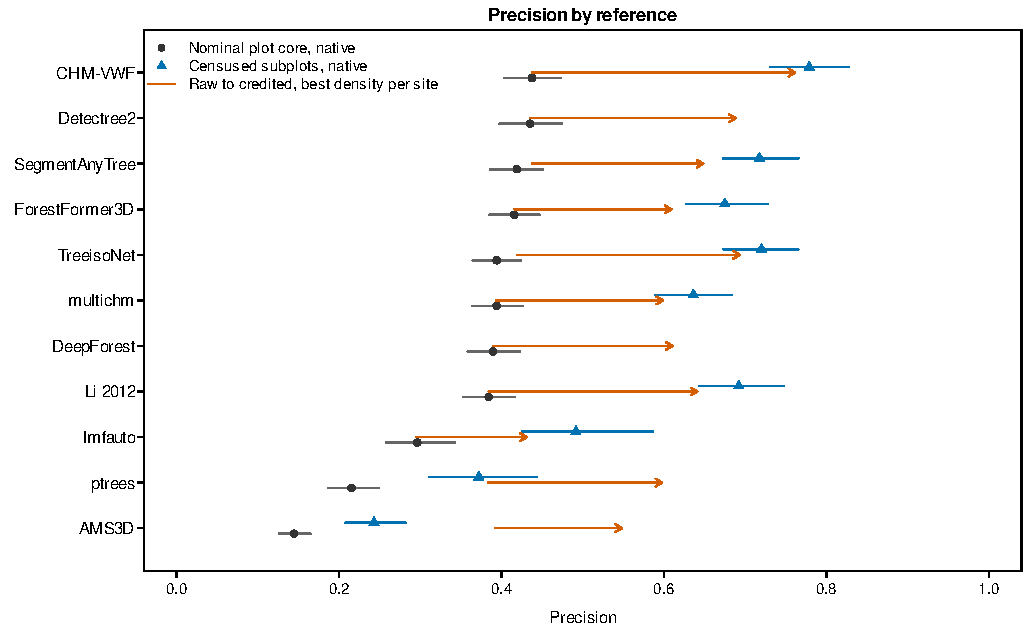
\includegraphics[width=\textwidth]{figures/figure_s1.pdf}\par}
\medskip
\textbf{Figure S1.} Precision under three references. Circles: nominal plot core at
native density, 106 plots, with 95\% intervals. Triangles: censused subplots at
native density, 57 plots, with 95\% intervals. Arrows: raw to credited precision
at the density each detector scores best at per site (Table~S5), except CHM-VWF,
whose arrow is at native density. For the other LiDAR detectors except Li 2012
that density is a sparser density level at one or more sites, and the arrows of
AMS3D, \texttt{ptrees}, TreeisoNet and SegmentAnyTree start visibly away from the
native-density circle. Circles and triangles are on different plot sets; on the
same 57 plots CHM-VWF's nominal precision is 0.48.
\end{figure}

\section*{S21. Sensitivity of the evaluation}

Detail of the sensitivity analyses of Section~4.6 of the manuscript: chance
agreement at two radii, alternative matchers and radii, stem-position jitter,
the gap between census and flight, and the tuning of the baseline. Source:
\href{https://github.com/devakellc/lidar-tree-benchmark/blob/main/results/matcher-robustness-results.md}{matcher-robustness study} for chance
agreement and matching, \href{https://github.com/devakellc/lidar-tree-benchmark/blob/main/results/positional-uncertainty-results.md}{positional
uncertainty}, \href{https://github.com/devakellc/lidar-tree-benchmark/blob/main/results/temporal-sensitivity-results.md}{temporal
sensitivity} and the
\href{https://github.com/devakellc/lidar-tree-benchmark/blob/main/results/calibration-validation-results.md}{calibration/validation study}.

\textbf{Chance agreement.} At native density the null reproduces 70 to 79\% of every
detector's F1 at 4 m and 49 to 60\% at 2 m (67 to 79\% and 44 to 66\% below native
density; 69 to 77\% and 44 to 64\% at the QL2 level). Every match within 2 m is
also a match within 4 m, so a detector's share of stems found by skill cannot be
larger at 2 m than at 4 m. The F1 above the null grows from 4 to 2 m for ten of
the eleven detectors (CHM-VWF 0.133 to 0.176; Fig.~S2d), but under the
correction of Section~4.2 of the manuscript the F1 above the null is the skill
share times the headroom, so most of that growth is expected as the null falls:
with constant skill CHM-VWF's 0.133 would become 0.162, and for the two
segmenters the growth equals the expectation. The test of the correction is
therefore corrected F1 itself, which is higher at 2 m for seven of the eleven
detectors, unchanged for the two segmenters (0.215 and 0.214 for ForestFormer3D,
0.229 and 0.228 for SegmentAnyTree) and lower for the two RGB detectors;
CHM-VWF's rises from 0.195 to 0.211 and that of the other detectors changes by
up to 0.03, so the segmenters' corrected leads shrink at 2 m (Table~S12a):
ForestFormer3D's from +0.020 to +0.003 [$-$0.014, +0.021] and SegmentAnyTree's
from +0.034 to +0.017 [$-$0.001, +0.033]. Their leads in F1 above the null are
smaller (+0.005 and 0.000 for ForestFormer3D, +0.017 and +0.010 for
SegmentAnyTree). Of these eight estimates for the two segmenters, only
SegmentAnyTree's corrected lead at 4 m has an interval that excludes zero, and
only narrowly. In California both corrected leads hold at 2 m (+0.049 [+0.028,
+0.071] and +0.054 [+0.023, +0.082]); in Washington both are level with the
baseline ($-$0.018 [$-$0.042, +0.007] and +0.000 [$-$0.020, +0.019]). At the QL2 level
the corrected leads of the four leading detectors are $-$0.023 to +0.024 at 2 m;
only \texttt{multichm}'s ($-$0.023 [$-$0.044, $-$0.001]) and TreeisoNet's (+0.024 [+0.004,
+0.042]) exclude zero, both narrowly. The null's constants do not drive these
results: on the five sites an independent set of 200 offsets changes any null F1
by at most 0.002 and any corrected F1 lead by at most 0.002, and minimum shifts
of 6 m or 12 m instead of 8 m change the segmenters' native corrected leads by
at most 0.001 (Section~S12).

\textbf{Matching.} In observed F1, the alternative matchers leave the leads in place;
a tighter radius does not (Fig.~S2). Hungarian assignment raises every
detector's native F1, by at most 0.03, and by at most 0.04 with a crown-scaled
tolerance; the soft three-dimensional cost moves detectors by $-$0.02 to +0.01.
The two segmenters lead CHM-VWF by 0.03 to 0.06 under every matcher and at radii
of 3 to 5 m, and over that range the ranking of the twelve detectors, SAM2Point
included, keeps a Kendall $\tau$ of at least 0.85 with the ranking under the default
matcher. Over all detectors and densities, 2 m lowers F1 by 0.04 to 0.16 (0.05
to 0.14 at native density) and 5 m raises it by 0.01 to 0.04, for every detector
in the same direction but not by the same amount. At 2 m SegmentAnyTree keeps a
narrow observed lead of +0.026 [+0.009, +0.043] over CHM-VWF, ForestFormer3D's
falls to +0.012 [$-$0.008, +0.031], and $\tau$ falls to 0.79. The loss is in the
replication region: in California both leads stay at 0.06 to 0.07 at 2 m, while
in Washington they are 0.02 at 3 m (+0.024 [$-$0.004, +0.051] and +0.022 [$-$0.001,
+0.042]), and at 2 m ForestFormer3D is 0.010 behind the baseline [$-$0.036,
+0.016] and SegmentAnyTree 0.012 ahead [$-$0.008, +0.029]. \texttt{multichm} depends most
on the radius: at native density it goes from level with CHM-VWF at 4 m to 0.032
behind it at 2 m [$-$0.053, $-$0.011], and at 2.2 pulses/m\textsuperscript{2} its lead over CHM-VWF
falls from +0.045 at 4 m to +0.026 at 3 m and +0.016 [$-$0.007, +0.039] at 2 m,
while the three learned detectors keep +0.041 to +0.065. At the QL2 level,
scored with the same grid, \texttt{multichm}'s lead falls from +0.058 at 4 m to +0.043
at 3 m and +0.011 [$-$0.010, +0.033] at 2 m, while the learned detectors keep
+0.030 to +0.065 at 2 m.

\textbf{Stem position.} Independent jitter of each stem by its recorded uncertainty
gives 90\% bands at most 0.008 F1 wide, a quarter or less of the plot-sampling
intervals, and the two segmenters beat CHM-VWF in every one of 200 draws. A
shared offset of a whole plot is not tested and would act like a change of
radius.

\textbf{Temporal gap.} Scoring only against stems measured in the flight year, on the
44 plots that have any, raises recall by 0.01 to 0.04 for most detectors and
lowers precision for all, because the stems measured in other years still stand
and their detections now count as errors; F1 on this cut is a lower bound.
SegmentAnyTree keeps a narrow lead over CHM-VWF on the cut (+0.039 [+0.008,
+0.069], against +0.050 with all stems on the same plots), clear in California
(+0.113 [+0.031, +0.196]) and not distinguishable from zero in Washington
(+0.025 [$-$0.002, +0.053]). ForestFormer3D's lead vanishes overall (+0.000
[$-$0.034, +0.034], against +0.034), holds in California (+0.075 [+0.016, +0.135])
and is negative in Washington, within an interval that spans zero ($-$0.018
[$-$0.061, +0.020]). The paired change of each lead between the two references has
its own interval: $-$0.034 [$-$0.060, $-$0.014] for ForestFormer3D on the 44 plots
($-$0.038 [$-$0.072, $-$0.013] in Washington) and $-$0.011 [$-$0.021, $-$0.003], a narrow
change, for SegmentAnyTree, so the cut moves ForestFormer3D's lead and barely
moves SegmentAnyTree's.

The cut penalises a detector for finding the stems it removes, so a second
scoring, added after an internal review, ignores those stems instead: a
detection that the matching pairs with a stem measured in another year counts as
neither a true nor a false positive. ForestFormer3D's lead is then +0.006
[$-$0.026, +0.037] on the 44 plots, a change of $-$0.028 [$-$0.050, $-$0.012] from the
reference with all stems, and $-$0.011 [$-$0.050, +0.024] in Washington;
SegmentAnyTree's is +0.041 [+0.010, +0.069]. The penalty thus accounts for 0.006
of the 0.034 that ForestFormer3D's lead loses on the cut. The rest lies in which
stems the reference holds: ForestFormer3D's matching pairs 69\% of the 239 stems
measured in other years and 65\% of the flight-year stems, CHM-VWF's 35\% and 53\%,
and 45\% of the stems measured in other years are understory, against 18\% of the
flight-year stems. ForestFormer3D's lead on these plots therefore rests largely
on the stems measured in other years, whose year the cut cannot separate from
their make-up, and in the replication region it is not robust to the reference
window. Under this scoring recall still rises for eight of the twelve detectors,
by 0.014 to 0.039. Source: \href{https://github.com/devakellc/lidar-tree-benchmark/blob/main/results/temporal-sensitivity-results.md}{temporal
sensitivity}.

\textbf{Tuning.} Tuning the baseline's resolution and window on calibration plots
yields held-out F1 within a few hundredths of the fixed configuration's F1 on
all of a site's plots (Table~S9); the two are not scored on the same plots, so
this is a check of magnitude rather than a paired comparison. The best cell of
the grid beats the fixed configuration in sample by 0.006 to 0.016.

\begin{figure}[!ht]
{\centering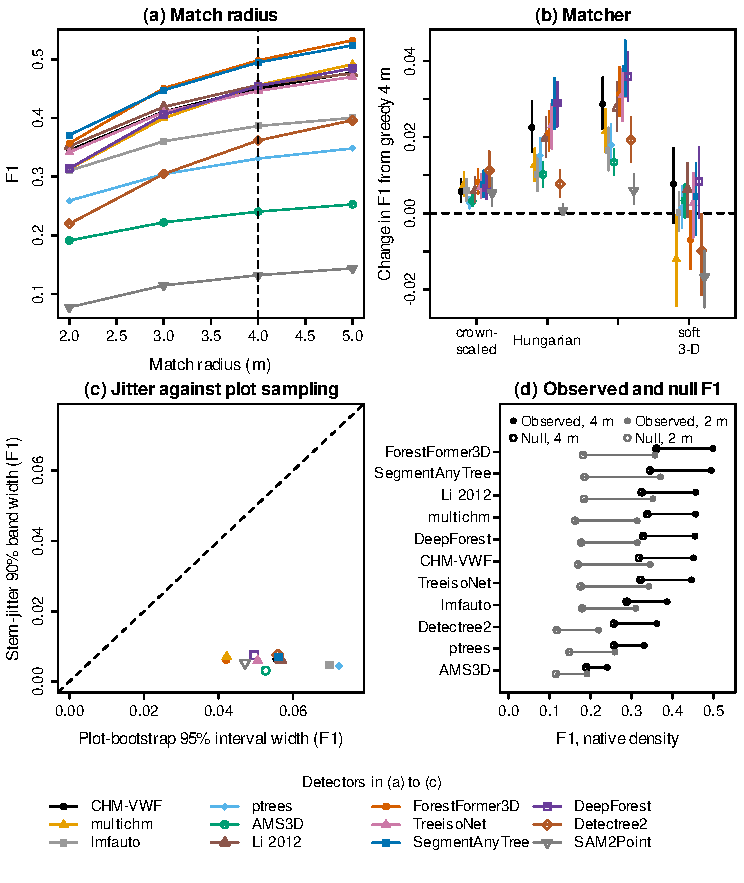
\includegraphics[width=0.75\textwidth]{figures/figure_s2.pdf}\par}
\medskip
\textbf{Figure S2.} Sensitivity of the evaluation at native density, five sites. (a)
F1 against the match radius. (b) Change in F1 from the default greedy 4 m
matcher under four alternatives, with 95\% intervals. (c) Width of the 90\%
stem-jitter band against the width of the 95\% plot-bootstrap interval for each
detector. (d) Observed F1 and the F1 of randomly shifted copies of the same
detections (the null of Section~4.2 of the manuscript) at the 4 m and 2 m radii;
the segment between the open and the filled symbol is the F1 above the null.
SAM2Point is shown in (a) to (c) for completeness (Section~S10).
\end{figure}

\section*{S22. Compute cost}

Run times of the detectors at native density, on which the cost per square
kilometre in Table~2 of the manuscript rests. Timings depend on the machine, and
each is the wall time of one call: it includes R start-up and clip reading for
the classical detectors, and container start and model loading for the learned
ones. Source: \href{https://github.com/devakellc/lidar-tree-benchmark/blob/main/results/compute-cost-results.md}{compute cost}.

The classical detectors, TreeisoNet and Detectree2 take seconds per plot;
ForestFormer3D takes one to two minutes and SegmentAnyTree four to seven (Table~S22). For these two segmenters the plot size sets the time more than the number
of points does: ForestFormer3D takes 64 to 69 s on distributed plots and 98 to
104 s on tower plots, SegmentAnyTree 251 to 297 s and 411 to 445 s. Scaled by
the clip area (a tower clip of 90 m $\times$ 90 m is 0.0081 km\textsuperscript{2}), ForestFormer3D costs
about 3.4 GPU-hours per km\textsuperscript{2}, SegmentAnyTree about 14, TreeisoNet about 16 min
and the classical detectors a few CPU-minutes per km\textsuperscript{2}, before the tiling
overhead that whole-scene inference over larger areas would add.

{\footnotesize
\setlength{\tabcolsep}{3pt}
\renewcommand{\arraystretch}{1.15}
\begin{xltabular}{\textwidth}{llRrR}
\multicolumn{5}{@{}p{\textwidth}@{}}{\normalsize\textbf{Table S22.} Wall time and peak GPU memory per plot at native density on nine
plots (one tower and one distributed plot per site; SJER has only tower plots),
on an Intel Core i9-14900K and one NVIDIA RTX 5090. DeepForest predicts every
image tile of a site once, so its time is a per-site cost.} \\[4pt]
\toprule
Detector & Runs on & Median wall time (s) & Maximum (s) & Peak GPU memory (MiB) \\
\midrule
\endfirsthead
\multicolumn{5}{@{}l@{}}{\normalsize\textbf{Table S22} (continued)} \\[4pt]
\toprule
Detector & Runs on & Median wall time (s) & Maximum (s) & Peak GPU memory (MiB) \\
\midrule
\endhead
\bottomrule
\endfoot
CHM-VWF & CPU & 2.9 & 3.6 & --- \\
\texttt{multichm} & CPU & 6.0 & 7.6 & --- \\
\texttt{lmfauto} & CPU & 2.3 & 2.5 & --- \\
\texttt{ptrees} & CPU & 3.2 & 3.5 & --- \\
AMS3D & CPU & 5.0 & 53.3 & --- \\
Li 2012 & CPU & 3.7 & 9.2 & --- \\
TreeisoNet & GPU & 7.9 & 8.6 & 2,886 \\
ForestFormer3D & GPU & 97.9 & 103.7 & 1,944 \\
SegmentAnyTree & GPU & 411.1 & 445.4 & 888 \\
Detectree2 & CPU & 8.1 & 9.2 & --- \\
DeepForest & GPU & 265.7 & 326.3 & 962 \\
\end{xltabular}
}

\section*{S23. A detector added after the tables were fixed}

ForestMamba \citep{nguyen2026forestmamba} is a fork of the ForestFormer3D code that
replaces its encoder context and transformer query decoder with Mamba
state-space layers and seeds its tree queries at the peaks of a canopy height
model built from the voxels it labels as tree; its authors report a
FOR-instanceV2 weighted-mean F1 of 83.4 against ForestFormer3D's 82.3 for the
paper's model, and their repository says the released checkpoint scores higher.
Its release checkpoint (\texttt{v6\_epoch\_1500\_fix.pth} from the authors' release
folder, pinned by SHA-256 in the repository, with the code at upstream commit
f0c5239), trained on FOR-instanceV2, was ported to current PyTorch and prebuilt
Mamba kernels, both newer than the upstream pins, in a container built on the
benchmark's ForestFormer3D image; the port reproduces the authors' published
predictions of the same checkpoint on three FOR-instanceV2 test scenes within
the model's run-to-run variation. It was run zero-shot on the fixed evaluation
clips of the five sites, the QL2 level included, with the settings of Table~S15,
after the tables of this paper were fixed, and compared with ForestFormer3D,
SegmentAnyTree, TreeisoNet and CHM-VWF by the same code, population, matching
rule and shift null, which reproduces those four detectors' numbers exactly.
None of the result tables or figures changes. The detector counts of the
abstract and Section~1 of the manuscript refer to the eleven detectors of its
Table~2, and ``the learned detectors'' elsewhere in the paper to the three of its
Section~4.1; both leave it out, as do the rank correlations of Sections~4.4 and
5.2, which are stated for the eight detectors run at every density (Table~4),
and the density routing of Section~S25, whose candidates are the same eight. The
run asks whether a fourth learned detector fits the pattern of the result
tables. Source: \href{https://github.com/devakellc/lidar-tree-benchmark/blob/main/results/forestmamba-results.md}{ForestMamba benchmark} and
\href{https://github.com/devakellc/lidar-tree-benchmark/blob/main/gpu/forestmamba-sm120/README.md}{ForestMamba runtime}.

At native density ForestMamba scores F1 0.442 [0.421, 0.464], $-$0.056 [$-$0.078,
$-$0.032] against ForestFormer3D and level with TreeisoNet and CHM-VWF, because it
places 0.78 detections per field stem, the fewest of the learned detectors, at
the highest precision (0.480) and the lowest recall (0.410) of the five
detectors compared; it recalls 0.247 of the understory stems, 0.045 [0.007,
0.085] above the null, narrowly, against ForestFormer3D's 0.454 and 0.094.
Thinning raises its detection count to about one per stem: it is level with
ForestFormer3D at every decimated density level, 0.454 [0.433, 0.475] against
0.452 at the QL2 level, and loses 0.034 [0.011, 0.059] F1 from native density to
0.6 pulses/m\textsuperscript{2} (0.022, level, in a repeat run), against ForestFormer3D's 0.078
and SegmentAnyTree's 0.367. Its leads over the baseline with its pre-declared
smoothing rule at the decimated density levels, 0.06 to 0.07 F1 from 4.4 to 1.1
pulses/m\textsuperscript{2}, follow that rule as the other detectors' do (Section~5.2 of the
manuscript; Section~S16): against the baseline without its smoothing, a
comparison made before that baseline was run at the QL2 level, it is $-$0.011 to
+0.010 from native density to 1.1 pulses/m\textsuperscript{2} and $-$0.023 [$-$0.041, $-$0.006] at 0.6
pulses/m\textsuperscript{2}, narrowly, and level there in the repeat run. Randomly shifted copies
of its detections reach 69 to 72\% of its F1, 69\% at native density against 70 to
79\% for the eleven detectors of Table~3 of the manuscript. Corrected for chance
it is level with ForestFormer3D at every density level; against the baseline
with its pre-declared smoothing rule its corrected lead is +0.040 [+0.016,
+0.066] at 4.4 pulses/m\textsuperscript{2}, narrow at 2.2 and 1.1 pulses/m\textsuperscript{2} (+0.028 and +0.021),
+0.020 [$-$0.001, +0.043], level, at the QL2 level, like the other learned
detectors' there (+0.014 to +0.017), and level at native density and 0.6
pulses/m\textsuperscript{2} (+0.002 and +0.000). Inside censused subplots its native-density F1,
0.564 [0.526, 0.601], is the lowest of the five, level with CHM-VWF's. Its
semantic head labels 19\% of the vegetation points as wood at native density and
86\% at 0.6 pulses/m\textsuperscript{2}, so the sparse airborne clips lie outside its training
domain, yet its instance head keeps about one detection per stem at every
decimated density level, unlike SegmentAnyTree's grouping stage (Section~6.2 of
the manuscript). Its runs are not bit-repeatable: a second run at the native and
sparsest density levels changed the counts of 79 to 86\% of the cells, pooled F1
by at most 0.007 and single sites by up to 0.023, a variation the main runs of
ForestFormer3D and TreeisoNet did not measure. It takes a median 55 s per plot
on the nine plots of Table~S22, against 92 s for ForestFormer3D re-timed in the
same session.

\section*{S24. Repository checks of recent models}

Dated checks of the recent models of Section~2.3 of the manuscript:
SegmentAnyTreeV2 \citep{wielgosz2026segmentanytreev2}, SelectAnyTree
\citep{nguyen2026selectanytree}, ForestMamba \citep{nguyen2026forestmamba}, ForPT
\citep{yue2026toward}, ITS-Net \citep{li2026itsnet} and ForestQuery
\citep{zhan2026forestquery}, none of which reports performance at 1 to 8 pulses/m\textsuperscript{2}.
Source: the cited papers and their repositories; the \href{https://github.com/devakellc/lidar-tree-benchmark/blob/main/docs/paper-proposal.md}{paper
proposal} records the repository checks.

On 21 October 2026 SegmentAnyTreeV2 still announced its weights on acceptance,
and the repositories of SelectAnyTree and ForestQuery held no code or
checkpoint; ForPT's repository, public since 9 October 2026, held code and
linked eleven Hugging Face checkpoints for pretraining, semantic segmentation,
species and age but none for instance segmentation; and ITS-Net's repository,
created in November 2025, held code without a checkpoint. The statements of
absence in Sections~2.1 to 2.3 of the manuscript rest on a scan of about ninety
primary sources completed on 30 September 2026, a literature check completed on
21 October 2026 and those repository checks, except ForestMamba's and
ForestQuery's, which rest on their papers; ForestQuery was posted on 2 October
2026, after the scan. ForestMamba, a fork of the ForestFormer3D code with Mamba
state-space layers and canopy-height query seeding, was not among the sources of
that scan; it has public code and weights, was run on the same clips in October
2026, after the tables were fixed, and is reported in Section~S23. The harness
took it as a fourth learned detector, with its own container and driver but no
change to the clips, population, matching rule or null.

A repeat of the repository checks on 16 November 2026 found the same state for
all six models. Two further models with public weights came to our notice then
and were not run: TreeLite3D \citep{rizaldy2026labelefficient} and ForestSeg3D
\citep{zhang2026forestseg3d}. A public repository of code and results without a
paper, whose only commit is dated 11 November 2026
\citep{mallacampoverde2026pretrained}, scores the released SegmentAnyTree,
ForestFormer3D and TreeLite3D weights and two classical methods on 22 alpine ALS
plots against 1,437 field-inventoried trees. It reports the score of uniformly
placed detections, greedy against optimal matching, crown strata and thinning by
pulse of its denser site from a median of 118 to 30 points/m\textsuperscript{2}. The statements of
absence in Sections~2.1 and 2.2 of the manuscript are therefore limited to
published work.

\section*{S25. Density routing by band and region}

The decision table behind the guidance of Section~6.1 of the manuscript answers
its RQ4 from the scores of the main tables, without re-running any detector. It
routes each cell, one plot at one density level, by the first-return density of
its plot core (Section~S26), as a user would route a tile by its measured
density: band A at 8 pulses/m\textsuperscript{2} or more (QL1 or denser), B from 2 to below 8 (QL2
to QL1) and C below 2 (below QL2). In each band the GPU route runs the
candidate, among the eight detectors run at every density, with the highest
pooled F1 on the band's California cells, and the CPU route the best of the five
classical ones (CHM-VWF, \texttt{multichm}, \texttt{lmfauto}, \texttt{ptrees} and AMS3D); the
Washington cells are the held-out check. The native-only choice is each route's
California best at the native level and the single choice its California best
over every cell, each used at every density. The bands, the candidate sets, the
selection rule and the comparisons were chosen after the five-site results were
known, so the analysis is post hoc; only the selection of the detectors is blind
to Washington, and the Washington best, chosen on the data it is compared on, is
descriptive. Table~S25a gives the decision table and its held-out check; the
tables after it give the bands, every candidate in every band and region, each
Washington pick against the other candidates of its band and the native-only
choice against the route. The last two tables pool every cell: each route,
choice and fixed detector, and the GPU route against each fixed detector and the
other choices.

Corrected F1 is at the 4 m radius, and intervals are 95\% plot-bootstrap
intervals over the master tables' resamples, paired for differences. California
scores are in sample, for the selection and for the detector settings. Band C
holds decimated cells only, and the comparison with native sparse flights
suggests that decimation is optimistic (Section~5.6 of the manuscript); CHM-VWF
keeps its pre-declared smoothing rule, which reads whole-clip density, so that 8
of the 25 native cells of band B ran without the smoothing and one native cell
of band A with it; precision is that of the nominal plot core, a lower bound.
Pooled over every cell, the six levels weigh equally, each stem counting once
per level, whereas a national archive has another mix of densities. Every
candidate's F1 and corrected F1 at every density level, at the five sites and in
each region, equal those of the master tables and of the chance-agreement
scoring exactly, intervals included. Source: \href{https://github.com/devakellc/lidar-tree-benchmark/blob/main/results/density-routing-results.md}{density-routing
study}, which also compares the CPU route
and the GPU native-only choice with every fixed detector over all cells.

With a GPU the route runs SegmentAnyTree from the QL2 floor up and \texttt{multichm}
below it, but the development data cannot separate its picks above the floor
from their runners-up (Table~S25a). On the California cells SegmentAnyTree leads
ForestFormer3D by 0.009 F1 at QL1 density or denser and by 0.002 between the QL2
and QL1 floors, each with a paired interval that includes zero, and \texttt{multichm}
is level with it in both bands. The pick between the floors also depends on how
density is measured: with the bands drawn on whole-clip density it was
ForestFormer3D, by less than 0.002 F1 over \texttt{multichm} (below). Below the
QL2 floor \texttt{multichm} narrowly leads AMS3D in F1, by 0.030, and not in corrected
F1. With only a CPU the route runs \texttt{multichm} in every band, so it is a single
detector. Its California leads over CHM-VWF above the QL2 floor, 0.063 and,
narrowly, 0.056 F1, include zero in corrected F1.

On the held-out Washington cells the GPU picks above the QL2 floor are the best
candidates of their bands, with ForestFormer3D level with them in both and
TreeisoNet between the floors. Below the floor \texttt{multichm} is level in F1 with
ForestFormer3D, TreeisoNet and AMS3D, and 0.026 behind TreeisoNet, the
Washington best, within an interval that includes zero. In corrected F1 it
trails TreeisoNet by 0.043 and, narrowly, ForestFormer3D and AMS3D by 0.022. The
CPU pick trails CHM-VWF at QL1 density or denser, narrowly in F1, by 0.035, and
by 0.056 in corrected F1. Over every Washington cell the GPU route is 0.014 F1
behind the per-band Washington best, an interval that includes zero, and 0.023
[0.011, 0.035] behind it in corrected F1 (Table~S25i). These bests are chosen on
the same data, so the gaps overstate what a choice made without the Washington
data could recover.

Routing pays off where it keeps SegmentAnyTree off clouds below the QL2 floor.
The GPU native-only choice is SegmentAnyTree, which won the native-density
comparison in California by 0.001 F1 over ForestFormer3D, so above the floor the
route and the native-only choice are the same detector. Below the floor the
route's \texttt{multichm} beats it by 0.080 [0.058, 0.103] F1 in Washington and 0.144
in California; in corrected F1 the gain is 0.069 in California and, within an
interval that includes zero, 0.012 in Washington (Table~S25g). Over every
Washington cell the route therefore gains 0.031 F1 over the native-only choice
and is level with it in corrected F1 (+0.003; Table~S25i).

Routing adds no accuracy over the best single learned detector. Run at every
density, ForestFormer3D is level with the GPU route, which leads it by +0.003
[$-$0.006, +0.012] F1 on the five sites (Table~S25i) and trails it by 0.003 in
Washington; in California, where the picks were selected, the route leads it
narrowly, by 0.017. TreeisoNet run at every density is also level with the route
in Washington but behind it in California; both detectors were singled out after
seeing the density series. The single choice by the routes' own rule is
\texttt{multichm}, which the GPU route leads in Washington by 0.022 F1 and 0.025
corrected F1.

Two limits bear on the table. The margins that decide the GPU picks above the
floor, 0.002 and 0.009 F1, are of the size of the run-to-run variation measured
for ForestMamba (0.007 F1; Section~S23) and not measured for ForestFormer3D. And
every cell below native density is a thinned copy of a native cloud, pooled with
equal weight per level, whereas a national archive has native sparse clouds and
another mix of densities.

{\scriptsize
\setlength{\tabcolsep}{3pt}
\renewcommand{\arraystretch}{1.15}
\begin{xltabular}{\textwidth}{>{\hsize=0.72\hsize\linewidth=\hsize}Lll>{\hsize=1.82997\hsize\linewidth=\hsize}L>{\hsize=0.63\hsize\linewidth=\hsize}L>{\hsize=0.63\hsize\linewidth=\hsize}L>{\hsize=0.87\hsize\linewidth=\hsize}L>{\hsize=1.32\hsize\linewidth=\hsize}L}
\multicolumn{8}{@{}p{\textwidth}@{}}{\normalsize\textbf{Table S25a.} The decision table and its held-out check.
Each cell, one plot at one density level, is routed by the first-return density
of its plot core; in each band a route runs the candidate with the highest
pooled F1 on the band's California cells, among the eight detectors run at every
density (GPU) or the five classical ones (CPU). Margin: the pick's paired F1
difference to the runner-up on the California cells. Washington is the held-out
region; corrected F1 is at 4 m. Level with the pick: the candidates whose paired
F1 difference to the pick on the Washington cells has an interval that includes
zero. Pick minus Washington best: paired differences, in F1 and in corrected F1,
to the candidate with the highest F1 on the Washington cells, which is chosen on
the same data and is descriptive; --- when the pick is that candidate. Tables~S25c to S25e give every candidate by band.} \\[4pt]
\toprule
Band (first-return pulses/m\textsuperscript{2}) & Compute & Detector to run & California F1; margin over the runner-up & Washington F1 & Washington corrected F1 & Level with the pick in Washington & Pick minus Washington best: F1; corrected F1 \\
\midrule
\endfirsthead
\multicolumn{8}{@{}l@{}}{\normalsize\textbf{Table S25a} (continued)} \\[4pt]
\toprule
Band (first-return pulses/m\textsuperscript{2}) & Compute & Detector to run & California F1; margin over the runner-up & Washington F1 & Washington corrected F1 & Level with the pick in Washington & Pick minus Washington best: F1; corrected F1 \\
\midrule
\endhead
\bottomrule
\endfoot
QL1 or denser (A: $\geq$ 8) & GPU & SegmentAnyTree & 0.456 [0.393, 0.518]; +0.009 [$-$0.028, +0.043] over ForestFormer3D & 0.518 [0.484, 0.550] & 0.216 [0.189, 0.244] & ForestFormer3D & --- \\
QL1 or denser (A: $\geq$ 8) & CPU & \texttt{multichm} & 0.425 [0.383, 0.472]; +0.063 [+0.033, +0.093] over CHM-VWF & 0.454 [0.427, 0.480] & 0.133 [0.108, 0.160] & \texttt{lmfauto} & CHM-VWF: $-$0.035 [$-$0.062, $-$0.005]; $-$0.056 [$-$0.082, $-$0.030] \\
QL2 to QL1 (B: 2 to \textless{} 8) & GPU & SegmentAnyTree & 0.433 [0.393, 0.475]; +0.002 [$-$0.024, +0.031] over ForestFormer3D & 0.498 [0.470, 0.522] & 0.192 [0.164, 0.221] & ForestFormer3D, TreeisoNet & --- \\
QL2 to QL1 (B: 2 to \textless{} 8) & CPU & \texttt{multichm} & 0.424 [0.385, 0.465]; +0.056 [+0.003, +0.108] over CHM-VWF & 0.459 [0.439, 0.480] & 0.149 [0.126, 0.173] & \texttt{ptrees} & \texttt{ptrees}: $-$0.001 [$-$0.029, +0.029]; $-$0.016 [$-$0.041, +0.011] \\
Below QL2 (C: \textless{} 2) & GPU & \texttt{multichm} & 0.424 [0.390, 0.460]; +0.030 [+0.003, +0.057] over AMS3D & 0.450 [0.429, 0.472] & 0.129 [0.110, 0.150] & ForestFormer3D, TreeisoNet, AMS3D & TreeisoNet: $-$0.026 [$-$0.057, +0.006]; $-$0.043 [$-$0.064, $-$0.021] \\
Below QL2 (C: \textless{} 2) & CPU & \texttt{multichm} & 0.424 [0.390, 0.460]; +0.030 [+0.003, +0.057] over AMS3D & 0.450 [0.429, 0.472] & 0.129 [0.110, 0.150] & AMS3D & AMS3D: $-$0.000 [$-$0.027, +0.026]; $-$0.022 [$-$0.041, $-$0.003] \\
\end{xltabular}
}

An earlier version of this analysis drew the bands on whole-clip density. Core
density moves 55 of the 636 cells to another band, 53 of them to a sparser one:
California holds 35, 115 and 108 cells in bands A, B and C against 37, 132 and
89 before, and Washington 46, 129 and 203 against 51, 149 and 178. Every pick is
the same except the GPU pick of band B, which was ForestFormer3D (California F1
0.428, against 0.426 for \texttt{multichm} and 0.417 for SegmentAnyTree) and is now
SegmentAnyTree (0.433 against ForestFormer3D's 0.431). Neither choice separates
from the other under either definition. Below the QL2 floor the route's gain
over the native-only choice in Washington was 0.101 [0.077, 0.126] F1 and 0.024
[0.006, 0.041] corrected F1 with whole-clip bands, and is 0.080 [0.058, 0.103]
and 0.012 [$-$0.006, 0.031] with core bands (Table~S25g).

{\scriptsize
\setlength{\tabcolsep}{3pt}
\renewcommand{\arraystretch}{1.15}
\begin{xltabular}{\textwidth}{LllrrrLrrrrrr}
\multicolumn{13}{@{}p{\textwidth}@{}}{\normalsize\textbf{Table S25b.} Bands of plot-core first-return density by scope, with the cells
of each density level, headed by the level's five-site median in pulses/m\textsuperscript{2}.
Stems sum the reference over a band's cells: a stem counts once at every level
whose cell falls in the band. Ranges are rounded; a cell's band uses its
unrounded density.} \\[4pt]
\toprule
Band & Pulses/m\textsuperscript{2} & Scope & Cells & Plots & Stems & Median pulses/m\textsuperscript{2} [range] & Cells at 9.8 & Cells at 4.4 & Cells at 2.2 & Cells at 1.8 & Cells at 1.1 & Cells at 0.6 \\
\midrule
\endfirsthead
\multicolumn{13}{@{}l@{}}{\normalsize\textbf{Table S25b} (continued)} \\[4pt]
\toprule
Band & Pulses/m\textsuperscript{2} & Scope & Cells & Plots & Stems & Median pulses/m\textsuperscript{2} [range] & Cells at 9.8 & Cells at 4.4 & Cells at 2.2 & Cells at 1.8 & Cells at 1.1 & Cells at 0.6 \\
\midrule
\endhead
\bottomrule
\endfoot
A (QL1 or denser) & $\geq$ 8 & five sites & 81 & 81 & 1,956 & 10.8 [8.08, 22.48] & 81 & 0 & 0 & 0 & 0 & 0 \\
B (QL2 to QL1) & 2 to \textless{} 8 & five sites & 244 & 106 & 5,548 & 3.8 [2.00, 7.96] & 25 & 106 & 86 & 27 & 0 & 0 \\
C (below QL2) & \textless{} 2 & five sites & 311 & 106 & 7,646 & 1.1 [0.39, 2.00] & 0 & 0 & 20 & 79 & 106 & 106 \\
A (QL1 or denser) & $\geq$ 8 & California & 35 & 35 & 567 & 12.1 [8.43, 22.48] & 35 & 0 & 0 & 0 & 0 & 0 \\
B (QL2 to QL1) & 2 to \textless{} 8 & California & 115 & 43 & 1,617 & 3.0 [2.05, 7.82] & 8 & 43 & 41 & 23 & 0 & 0 \\
C (below QL2) & \textless{} 2 & California & 108 & 43 & 1,788 & 1.1 [0.46, 1.98] & 0 & 0 & 2 & 20 & 43 & 43 \\
A (QL1 or denser) & $\geq$ 8 & Washington & 46 & 46 & 1,389 & 10.0 [8.08, 19.86] & 46 & 0 & 0 & 0 & 0 & 0 \\
B (QL2 to QL1) & 2 to \textless{} 8 & Washington & 129 & 63 & 3,931 & 4.0 [2.00, 7.96] & 17 & 63 & 45 & 4 & 0 & 0 \\
C (below QL2) & \textless{} 2 & Washington & 203 & 63 & 5,858 & 1.1 [0.39, 2.00] & 0 & 0 & 18 & 59 & 63 & 63 \\
\end{xltabular}
}

{\scriptsize
\setlength{\tabcolsep}{3pt}
\renewcommand{\arraystretch}{1.15}
\begin{xltabular}{\textwidth}{llLLLLLL}
\multicolumn{8}{@{}p{\textwidth}@{}}{\normalsize\textbf{Table S25c.} Every candidate by band, five sites (both regions): pooled F1
and corrected F1 with 95\% intervals. Picked in: the routes (GPU, CPU) and bands
(A, B, C) in which the detector is the pick.} \\[4pt]
\toprule
Detector & Picked in & A: F1 & A: corrected F1 & B: F1 & B: corrected F1 & C: F1 & C: corrected F1 \\
\midrule
\endfirsthead
\multicolumn{8}{@{}l@{}}{\normalsize\textbf{Table S25c} (continued)} \\[4pt]
\toprule
Detector & Picked in & A: F1 & A: corrected F1 & B: F1 & B: corrected F1 & C: F1 & C: corrected F1 \\
\midrule
\endhead
\bottomrule
\endfoot
ForestFormer3D &  & 0.493 [0.470, 0.517] & 0.214 [0.189, 0.238] & 0.472 [0.453, 0.493] & 0.205 [0.184, 0.227] & 0.441 [0.422, 0.460] & 0.170 [0.149, 0.192] \\
SegmentAnyTree & GPU AB & 0.497 [0.466, 0.528] & 0.235 [0.206, 0.264] & 0.477 [0.454, 0.498] & 0.219 [0.193, 0.244] & 0.350 [0.328, 0.369] & 0.126 [0.110, 0.144] \\
TreeisoNet &  & 0.446 [0.416, 0.476] & 0.182 [0.156, 0.209] & 0.448 [0.421, 0.473] & 0.190 [0.167, 0.212] & 0.447 [0.420, 0.474] & 0.181 [0.157, 0.204] \\
\texttt{multichm} & GPU C, CPU ABC & 0.445 [0.422, 0.470] & 0.166 [0.144, 0.192] & 0.448 [0.430, 0.466] & 0.180 [0.160, 0.201] & 0.443 [0.426, 0.462] & 0.155 [0.139, 0.173] \\
CHM-VWF &  & 0.451 [0.419, 0.481] & 0.192 [0.164, 0.223] & 0.399 [0.373, 0.423] & 0.178 [0.152, 0.206] & 0.385 [0.361, 0.409] & 0.162 [0.140, 0.187] \\
AMS3D &  & 0.224 [0.194, 0.256] & 0.058 [0.046, 0.071] & 0.342 [0.318, 0.366] & 0.111 [0.095, 0.129] & 0.437 [0.414, 0.461] & 0.164 [0.143, 0.187] \\
\texttt{ptrees} &  & 0.316 [0.278, 0.355] & 0.092 [0.071, 0.118] & 0.427 [0.399, 0.451] & 0.175 [0.153, 0.199] & 0.352 [0.331, 0.373] & 0.140 [0.120, 0.160] \\
\texttt{lmfauto} &  & 0.398 [0.356, 0.437] & 0.143 [0.114, 0.174] & 0.307 [0.276, 0.343] & 0.099 [0.080, 0.124] & 0.269 [0.241, 0.305] & 0.074 [0.059, 0.094] \\
\end{xltabular}
}

{\scriptsize
\setlength{\tabcolsep}{3pt}
\renewcommand{\arraystretch}{1.15}
\begin{xltabular}{\textwidth}{llLLLLLL}
\multicolumn{8}{@{}p{\textwidth}@{}}{\normalsize\textbf{Table S25d.} Every candidate by band, California: the selection data, in
sample.} \\[4pt]
\toprule
Detector & Picked in & A: F1 & A: corrected F1 & B: F1 & B: corrected F1 & C: F1 & C: corrected F1 \\
\midrule
\endfirsthead
\multicolumn{8}{@{}l@{}}{\normalsize\textbf{Table S25d} (continued)} \\[4pt]
\toprule
Detector & Picked in & A: F1 & A: corrected F1 & B: F1 & B: corrected F1 & C: F1 & C: corrected F1 \\
\midrule
\endhead
\bottomrule
\endfoot
ForestFormer3D &  & 0.447 [0.406, 0.493] & 0.255 [0.210, 0.309] & 0.431 [0.392, 0.475] & 0.257 [0.219, 0.305] & 0.390 [0.354, 0.428] & 0.214 [0.181, 0.251] \\
SegmentAnyTree & GPU AB & 0.456 [0.393, 0.518] & 0.265 [0.205, 0.334] & 0.433 [0.393, 0.475] & 0.263 [0.211, 0.315] & 0.279 [0.245, 0.313] & 0.152 [0.124, 0.182] \\
TreeisoNet &  & 0.361 [0.320, 0.406] & 0.190 [0.147, 0.243] & 0.364 [0.326, 0.406] & 0.202 [0.164, 0.246] & 0.369 [0.328, 0.411] & 0.199 [0.161, 0.241] \\
\texttt{multichm} & GPU C, CPU ABC & 0.425 [0.383, 0.472] & 0.230 [0.188, 0.280] & 0.424 [0.385, 0.465] & 0.235 [0.196, 0.277] & 0.424 [0.390, 0.460] & 0.220 [0.191, 0.255] \\
CHM-VWF &  & 0.362 [0.320, 0.403] & 0.195 [0.152, 0.244] & 0.368 [0.322, 0.416] & 0.233 [0.183, 0.290] & 0.353 [0.311, 0.394] & 0.213 [0.172, 0.259] \\
AMS3D &  & 0.206 [0.158, 0.271] & 0.077 [0.049, 0.116] & 0.317 [0.275, 0.362] & 0.152 [0.119, 0.190] & 0.393 [0.351, 0.438] & 0.197 [0.155, 0.245] \\
\texttt{ptrees} &  & 0.251 [0.206, 0.303] & 0.100 [0.067, 0.140] & 0.353 [0.314, 0.400] & 0.194 [0.155, 0.243] & 0.277 [0.244, 0.310] & 0.150 [0.124, 0.182] \\
\texttt{lmfauto} &  & 0.339 [0.291, 0.389] & 0.165 [0.117, 0.218] & 0.358 [0.312, 0.407] & 0.192 [0.149, 0.243] & 0.341 [0.296, 0.394] & 0.160 [0.118, 0.210] \\
\end{xltabular}
}

{\scriptsize
\setlength{\tabcolsep}{3pt}
\renewcommand{\arraystretch}{1.15}
\begin{xltabular}{\textwidth}{llLLLLLL}
\multicolumn{8}{@{}p{\textwidth}@{}}{\normalsize\textbf{Table S25e.} Every candidate by band, Washington: the held-out check.} \\[4pt]
\toprule
Detector & Picked in & A: F1 & A: corrected F1 & B: F1 & B: corrected F1 & C: F1 & C: corrected F1 \\
\midrule
\endfirsthead
\multicolumn{8}{@{}l@{}}{\normalsize\textbf{Table S25e} (continued)} \\[4pt]
\toprule
Detector & Picked in & A: F1 & A: corrected F1 & B: F1 & B: corrected F1 & C: F1 & C: corrected F1 \\
\midrule
\endhead
\bottomrule
\endfoot
ForestFormer3D &  & 0.512 [0.486, 0.538] & 0.193 [0.164, 0.221] & 0.491 [0.469, 0.514] & 0.176 [0.153, 0.200] & 0.459 [0.436, 0.481] & 0.151 [0.126, 0.178] \\
SegmentAnyTree & GPU AB & 0.518 [0.484, 0.550] & 0.216 [0.189, 0.244] & 0.498 [0.470, 0.522] & 0.192 [0.164, 0.221] & 0.370 [0.346, 0.394] & 0.118 [0.098, 0.139] \\
TreeisoNet &  & 0.488 [0.455, 0.520] & 0.178 [0.150, 0.207] & 0.492 [0.461, 0.521] & 0.184 [0.157, 0.210] & 0.476 [0.445, 0.504] & 0.173 [0.144, 0.203] \\
\texttt{multichm} & GPU C, CPU ABC & 0.454 [0.427, 0.480] & 0.133 [0.108, 0.160] & 0.459 [0.439, 0.480] & 0.149 [0.126, 0.173] & 0.450 [0.429, 0.472] & 0.129 [0.110, 0.150] \\
CHM-VWF &  & 0.489 [0.453, 0.525] & 0.189 [0.153, 0.230] & 0.412 [0.383, 0.443] & 0.151 [0.124, 0.182] & 0.395 [0.368, 0.423] & 0.143 [0.118, 0.172] \\
AMS3D &  & 0.233 [0.202, 0.264] & 0.047 [0.036, 0.059] & 0.354 [0.327, 0.382] & 0.090 [0.073, 0.108] & 0.450 [0.425, 0.477] & 0.151 [0.128, 0.180] \\
\texttt{ptrees} &  & 0.349 [0.300, 0.402] & 0.088 [0.061, 0.121] & 0.460 [0.428, 0.489] & 0.165 [0.140, 0.192] & 0.376 [0.351, 0.400] & 0.136 [0.111, 0.162] \\
\texttt{lmfauto} &  & 0.418 [0.366, 0.473] & 0.134 [0.103, 0.172] & 0.294 [0.258, 0.337] & 0.074 [0.056, 0.097] & 0.255 [0.225, 0.294] & 0.057 [0.043, 0.077] \\
\end{xltabular}
}

{\scriptsize
\setlength{\tabcolsep}{3pt}
\renewcommand{\arraystretch}{1.15}
\begin{xltabular}{\textwidth}{lllLLL}
\multicolumn{6}{@{}p{\textwidth}@{}}{\normalsize\textbf{Table S25f.} Washington: each pick against every other candidate of its band,
as paired differences, pick minus candidate, in F1 and corrected F1; the
Washington best is marked and is descriptive.} \\[4pt]
\toprule
Band & Route & Pick & Versus & Pick minus candidate, F1 & Pick minus candidate, corrected F1 \\
\midrule
\endfirsthead
\multicolumn{6}{@{}l@{}}{\normalsize\textbf{Table S25f} (continued)} \\[4pt]
\toprule
Band & Route & Pick & Versus & Pick minus candidate, F1 & Pick minus candidate, corrected F1 \\
\midrule
\endhead
\bottomrule
\endfoot
A & GPU & SegmentAnyTree & ForestFormer3D & +0.006 [$-$0.020, +0.027] & +0.023 [$-$0.001, +0.048] \\
A & GPU & SegmentAnyTree & TreeisoNet & +0.029 [+0.002, +0.054] & +0.038 [+0.008, +0.068] \\
A & GPU & SegmentAnyTree & \texttt{multichm} & +0.064 [+0.035, +0.087] & +0.083 [+0.058, +0.104] \\
A & GPU & SegmentAnyTree & CHM-VWF & +0.029 [+0.003, +0.054] & +0.026 [$-$0.008, +0.055] \\
A & GPU & SegmentAnyTree & AMS3D & +0.284 [+0.245, +0.317] & +0.168 [+0.141, +0.195] \\
A & GPU & SegmentAnyTree & \texttt{ptrees} & +0.169 [+0.118, +0.217] & +0.128 [+0.091, +0.162] \\
A & GPU & SegmentAnyTree & \texttt{lmfauto} & +0.099 [+0.034, +0.143] & +0.081 [+0.044, +0.109] \\
B & GPU & SegmentAnyTree & ForestFormer3D & +0.007 [$-$0.017, +0.026] & +0.017 [$-$0.007, +0.038] \\
B & GPU & SegmentAnyTree & TreeisoNet & +0.006 [$-$0.014, +0.027] & +0.009 [$-$0.015, +0.028] \\
B & GPU & SegmentAnyTree & \texttt{multichm} & +0.039 [+0.012, +0.062] & +0.044 [+0.016, +0.066] \\
B & GPU & SegmentAnyTree & CHM-VWF & +0.086 [+0.058, +0.110] & +0.041 [+0.015, +0.066] \\
B & GPU & SegmentAnyTree & AMS3D & +0.144 [+0.112, +0.171] & +0.102 [+0.077, +0.126] \\
B & GPU & SegmentAnyTree & \texttt{ptrees} & +0.038 [+0.016, +0.057] & +0.028 [+0.004, +0.048] \\
B & GPU & SegmentAnyTree & \texttt{lmfauto} & +0.204 [+0.154, +0.241] & +0.119 [+0.092, +0.143] \\
C & GPU & \texttt{multichm} & ForestFormer3D & $-$0.010 [$-$0.025, +0.006] & $-$0.022 [$-$0.037, $-$0.007] \\
C & GPU & \texttt{multichm} & SegmentAnyTree & +0.080 [+0.058, +0.103] & +0.012 [$-$0.006, +0.031] \\
C & GPU & \texttt{multichm} & TreeisoNet (Washington best) & $-$0.026 [$-$0.057, +0.006] & $-$0.043 [$-$0.064, $-$0.021] \\
C & GPU & \texttt{multichm} & CHM-VWF & +0.055 [+0.027, +0.082] & $-$0.014 [$-$0.036, +0.005] \\
C & GPU & \texttt{multichm} & AMS3D & $-$0.000 [$-$0.027, +0.026] & $-$0.022 [$-$0.041, $-$0.003] \\
C & GPU & \texttt{multichm} & \texttt{ptrees} & +0.074 [+0.047, +0.103] & $-$0.007 [$-$0.025, +0.012] \\
C & GPU & \texttt{multichm} & \texttt{lmfauto} & +0.195 [+0.156, +0.224] & +0.072 [+0.054, +0.088] \\
A & CPU & \texttt{multichm} & CHM-VWF (Washington best) & $-$0.035 [$-$0.062, $-$0.005] & $-$0.056 [$-$0.082, $-$0.030] \\
A & CPU & \texttt{multichm} & \texttt{lmfauto} & +0.035 [$-$0.019, +0.080] & $-$0.002 [$-$0.037, +0.027] \\
A & CPU & \texttt{multichm} & \texttt{ptrees} & +0.105 [+0.061, +0.149] & +0.045 [+0.008, +0.079] \\
A & CPU & \texttt{multichm} & AMS3D & +0.220 [+0.189, +0.252] & +0.086 [+0.061, +0.112] \\
B & CPU & \texttt{multichm} & CHM-VWF & +0.047 [+0.017, +0.080] & $-$0.002 [$-$0.028, +0.025] \\
B & CPU & \texttt{multichm} & \texttt{lmfauto} & +0.165 [+0.125, +0.201] & +0.075 [+0.054, +0.093] \\
B & CPU & \texttt{multichm} & \texttt{ptrees} (Washington best) & $-$0.001 [$-$0.029, +0.029] & $-$0.016 [$-$0.041, +0.011] \\
B & CPU & \texttt{multichm} & AMS3D & +0.105 [+0.079, +0.132] & +0.059 [+0.037, +0.081] \\
C & CPU & \texttt{multichm} & CHM-VWF & +0.055 [+0.027, +0.082] & $-$0.014 [$-$0.036, +0.005] \\
C & CPU & \texttt{multichm} & \texttt{lmfauto} & +0.195 [+0.156, +0.224] & +0.072 [+0.054, +0.088] \\
C & CPU & \texttt{multichm} & \texttt{ptrees} & +0.074 [+0.047, +0.103] & $-$0.007 [$-$0.025, +0.012] \\
C & CPU & \texttt{multichm} & AMS3D (Washington best) & $-$0.000 [$-$0.027, +0.026] & $-$0.022 [$-$0.041, $-$0.003] \\
\end{xltabular}
}

{\scriptsize
\setlength{\tabcolsep}{3pt}
\renewcommand{\arraystretch}{1.15}
\begin{xltabular}{\textwidth}{ll>{\hsize=0.69\hsize\linewidth=\hsize}Lll>{\hsize=1.14\hsize\linewidth=\hsize}L>{\hsize=1.16998\hsize\linewidth=\hsize}L}
\multicolumn{7}{@{}p{\textwidth}@{}}{\normalsize\textbf{Table S25g.} The native-only choice against the route, by band and scope: the
route minus the native-only choice in F1 and corrected F1, with paired
intervals. Bands A and B run the same detector in both, and with only a CPU both
are \texttt{multichm} in every band.} \\[4pt]
\toprule
Band & Compute & Native-only choice & Route's pick & Scope & Route minus native-only, F1 & Route minus native-only, corrected F1 \\
\midrule
\endfirsthead
\multicolumn{7}{@{}l@{}}{\normalsize\textbf{Table S25g} (continued)} \\[4pt]
\toprule
Band & Compute & Native-only choice & Route's pick & Scope & Route minus native-only, F1 & Route minus native-only, corrected F1 \\
\midrule
\endhead
\bottomrule
\endfoot
A & GPU & SegmentAnyTree & SegmentAnyTree & five sites & +0.000 [+0.000, +0.000] & +0.000 [+0.000, +0.000] \\
A & GPU & SegmentAnyTree & SegmentAnyTree & California & +0.000 [+0.000, +0.000] & +0.000 [+0.000, +0.000] \\
A & GPU & SegmentAnyTree & SegmentAnyTree & Washington & +0.000 [+0.000, +0.000] & +0.000 [+0.000, +0.000] \\
B & GPU & SegmentAnyTree & SegmentAnyTree & five sites & +0.000 [+0.000, +0.000] & +0.000 [+0.000, +0.000] \\
B & GPU & SegmentAnyTree & SegmentAnyTree & California & +0.000 [+0.000, +0.000] & +0.000 [+0.000, +0.000] \\
B & GPU & SegmentAnyTree & SegmentAnyTree & Washington & +0.000 [+0.000, +0.000] & +0.000 [+0.000, +0.000] \\
C & GPU & SegmentAnyTree & \texttt{multichm} & five sites & +0.094 [+0.074, +0.116] & +0.029 [+0.014, +0.046] \\
C & GPU & SegmentAnyTree & \texttt{multichm} & California & +0.144 [+0.108, +0.181] & +0.069 [+0.041, +0.100] \\
C & GPU & SegmentAnyTree & \texttt{multichm} & Washington & +0.080 [+0.058, +0.103] & +0.012 [$-$0.006, +0.031] \\
A & CPU & \texttt{multichm} & \texttt{multichm} & five sites & +0.000 [+0.000, +0.000] & +0.000 [+0.000, +0.000] \\
A & CPU & \texttt{multichm} & \texttt{multichm} & California & +0.000 [+0.000, +0.000] & +0.000 [+0.000, +0.000] \\
A & CPU & \texttt{multichm} & \texttt{multichm} & Washington & +0.000 [+0.000, +0.000] & +0.000 [+0.000, +0.000] \\
B & CPU & \texttt{multichm} & \texttt{multichm} & five sites & +0.000 [+0.000, +0.000] & +0.000 [+0.000, +0.000] \\
B & CPU & \texttt{multichm} & \texttt{multichm} & California & +0.000 [+0.000, +0.000] & +0.000 [+0.000, +0.000] \\
B & CPU & \texttt{multichm} & \texttt{multichm} & Washington & +0.000 [+0.000, +0.000] & +0.000 [+0.000, +0.000] \\
C & CPU & \texttt{multichm} & \texttt{multichm} & five sites & +0.000 [+0.000, +0.000] & +0.000 [+0.000, +0.000] \\
C & CPU & \texttt{multichm} & \texttt{multichm} & California & +0.000 [+0.000, +0.000] & +0.000 [+0.000, +0.000] \\
C & CPU & \texttt{multichm} & \texttt{multichm} & Washington & +0.000 [+0.000, +0.000] & +0.000 [+0.000, +0.000] \\
\end{xltabular}
}

{\scriptsize
\setlength{\tabcolsep}{3pt}
\renewcommand{\arraystretch}{1.15}
\begin{xltabular}{\textwidth}{LLLLLLL}
\multicolumn{7}{@{}p{\textwidth}@{}}{\normalsize\textbf{Table S25h.} Every cell pooled: F1 and corrected F1 of each route, choice and
fixed detector over the whole density series, by scope, with 95\% intervals. The
six levels weigh equally; the Washington best is descriptive.} \\[4pt]
\toprule
Policy or detector & Five sites, F1 & Five sites, corrected F1 & California, F1 & California, corrected F1 & Washington, F1 & Washington, corrected F1 \\
\midrule
\endfirsthead
\multicolumn{7}{@{}l@{}}{\normalsize\textbf{Table S25h} (continued)} \\[4pt]
\toprule
Policy or detector & Five sites, F1 & Five sites, corrected F1 & California, F1 & California, corrected F1 & Washington, F1 & Washington, corrected F1 \\
\midrule
\endhead
\bottomrule
\endfoot
GPU route & 0.463 [0.445, 0.481] & 0.189 [0.170, 0.209] & 0.432 [0.398, 0.471] & 0.245 [0.206, 0.289] & 0.475 [0.454, 0.496] & 0.162 [0.143, 0.184] \\
CPU route & 0.445 [0.428, 0.464] & 0.166 [0.150, 0.184] & 0.424 [0.389, 0.461] & 0.228 [0.195, 0.264] & 0.454 [0.434, 0.475] & 0.137 [0.119, 0.158] \\
Native-only choice, GPU & 0.428 [0.407, 0.447] & 0.180 [0.162, 0.199] & 0.388 [0.355, 0.424] & 0.224 [0.185, 0.267] & 0.444 [0.420, 0.465] & 0.159 [0.140, 0.182] \\
Native-only choice, CPU & 0.445 [0.428, 0.464] & 0.166 [0.150, 0.184] & 0.424 [0.389, 0.461] & 0.228 [0.195, 0.264] & 0.454 [0.434, 0.475] & 0.137 [0.119, 0.158] \\
Single choice, GPU & 0.445 [0.428, 0.464] & 0.166 [0.150, 0.184] & 0.424 [0.389, 0.461] & 0.228 [0.195, 0.264] & 0.454 [0.434, 0.475] & 0.137 [0.119, 0.158] \\
Single choice, CPU & 0.445 [0.428, 0.464] & 0.166 [0.150, 0.184] & 0.424 [0.389, 0.461] & 0.228 [0.195, 0.264] & 0.454 [0.434, 0.475] & 0.137 [0.119, 0.158] \\
Washington best per band, GPU (descriptive) & 0.466 [0.441, 0.489] & 0.203 [0.180, 0.224] & 0.409 [0.372, 0.449] & 0.235 [0.193, 0.283] & 0.489 [0.463, 0.514] & 0.185 [0.162, 0.211] \\
Washington best per band, CPU (descriptive) & 0.435 [0.412, 0.455] & 0.171 [0.151, 0.192] & 0.373 [0.339, 0.410] & 0.195 [0.159, 0.238] & 0.458 [0.434, 0.480] & 0.160 [0.138, 0.186] \\
ForestFormer3D & 0.460 [0.442, 0.477] & 0.189 [0.169, 0.209] & 0.415 [0.379, 0.453] & 0.237 [0.203, 0.278] & 0.478 [0.457, 0.498] & 0.166 [0.143, 0.189] \\
SegmentAnyTree & 0.428 [0.407, 0.447] & 0.180 [0.162, 0.199] & 0.388 [0.355, 0.424] & 0.224 [0.185, 0.267] & 0.444 [0.420, 0.465] & 0.159 [0.140, 0.182] \\
TreeisoNet & 0.447 [0.422, 0.472] & 0.185 [0.162, 0.206] & 0.366 [0.326, 0.405] & 0.199 [0.163, 0.241] & 0.483 [0.455, 0.510] & 0.177 [0.152, 0.204] \\
\texttt{multichm} & 0.445 [0.428, 0.464] & 0.166 [0.150, 0.184] & 0.424 [0.389, 0.461] & 0.228 [0.195, 0.264] & 0.454 [0.434, 0.475] & 0.137 [0.119, 0.158] \\
CHM-VWF & 0.401 [0.379, 0.423] & 0.172 [0.149, 0.195] & 0.361 [0.321, 0.402] & 0.218 [0.177, 0.263] & 0.415 [0.391, 0.442] & 0.152 [0.128, 0.181] \\
AMS3D & 0.346 [0.321, 0.369] & 0.113 [0.098, 0.129] & 0.308 [0.267, 0.354] & 0.143 [0.110, 0.178] & 0.362 [0.334, 0.389] & 0.099 [0.084, 0.117] \\
\texttt{ptrees} & 0.370 [0.348, 0.391] & 0.138 [0.122, 0.157] & 0.299 [0.268, 0.336] & 0.151 [0.122, 0.187] & 0.398 [0.375, 0.422] & 0.133 [0.114, 0.154] \\
\texttt{lmfauto} & 0.292 [0.265, 0.327] & 0.087 [0.071, 0.109] & 0.347 [0.304, 0.394] & 0.172 [0.130, 0.219] & 0.280 [0.249, 0.321] & 0.068 [0.052, 0.089] \\
\end{xltabular}
}

{\scriptsize
\setlength{\tabcolsep}{3pt}
\renewcommand{\arraystretch}{1.15}
\begin{xltabular}{\textwidth}{LLLLLLL}
\multicolumn{7}{@{}p{\textwidth}@{}}{\normalsize\textbf{Table S25i.} The GPU route minus each fixed detector and the other choices,
every cell, by scope, as paired differences in F1 and corrected F1 with 95\%
intervals.} \\[4pt]
\toprule
Versus & Five sites, F1 & Five sites, corrected F1 & California, F1 & California, corrected F1 & Washington, F1 & Washington, corrected F1 \\
\midrule
\endfirsthead
\multicolumn{7}{@{}l@{}}{\normalsize\textbf{Table S25i} (continued)} \\[4pt]
\toprule
Versus & Five sites, F1 & Five sites, corrected F1 & California, F1 & California, corrected F1 & Washington, F1 & Washington, corrected F1 \\
\midrule
\endhead
\bottomrule
\endfoot
ForestFormer3D & +0.003 [$-$0.006, +0.012] & +0.000 [$-$0.010, +0.010] & +0.017 [+0.002, +0.035] & +0.008 [$-$0.009, +0.027] & $-$0.003 [$-$0.014, +0.007] & $-$0.004 [$-$0.018, +0.008] \\
SegmentAnyTree & +0.035 [+0.026, +0.046] & +0.009 [+0.002, +0.017] & +0.045 [+0.031, +0.059] & +0.021 [+0.010, +0.033] & +0.031 [+0.019, +0.044] & +0.003 [$-$0.006, +0.012] \\
TreeisoNet & +0.016 [$-$0.002, +0.033] & +0.004 [$-$0.009, +0.019] & +0.067 [+0.039, +0.096] & +0.046 [+0.024, +0.071] & $-$0.008 [$-$0.029, +0.015] & $-$0.015 [$-$0.034, +0.002] \\
\texttt{multichm} & +0.018 [+0.009, +0.026] & +0.024 [+0.015, +0.032] & +0.008 [$-$0.005, +0.023] & +0.017 [$-$0.000, +0.036] & +0.022 [+0.010, +0.032] & +0.025 [+0.014, +0.034] \\
CHM-VWF & +0.062 [+0.042, +0.081] & +0.017 [$-$0.001, +0.034] & +0.072 [+0.032, +0.109] & +0.027 [$-$0.013, +0.065] & +0.060 [+0.035, +0.081] & +0.010 [$-$0.011, +0.026] \\
AMS3D & +0.117 [+0.097, +0.136] & +0.076 [+0.063, +0.089] & +0.124 [+0.095, +0.155] & +0.103 [+0.078, +0.130] & +0.113 [+0.090, +0.136] & +0.063 [+0.047, +0.078] \\
\texttt{ptrees} & +0.093 [+0.079, +0.107] & +0.051 [+0.040, +0.062] & +0.134 [+0.112, +0.155] & +0.094 [+0.075, +0.116] & +0.077 [+0.061, +0.092] & +0.029 [+0.016, +0.043] \\
\texttt{lmfauto} & +0.171 [+0.134, +0.201] & +0.102 [+0.083, +0.117] & +0.086 [+0.058, +0.112] & +0.073 [+0.049, +0.098] & +0.195 [+0.153, +0.227] & +0.094 [+0.075, +0.110] \\
Native-only choice, GPU & +0.035 [+0.026, +0.046] & +0.009 [+0.002, +0.017] & +0.045 [+0.031, +0.059] & +0.021 [+0.010, +0.033] & +0.031 [+0.019, +0.044] & +0.003 [$-$0.006, +0.012] \\
CPU route & +0.018 [+0.009, +0.026] & +0.024 [+0.015, +0.032] & +0.008 [$-$0.005, +0.023] & +0.017 [$-$0.000, +0.036] & +0.022 [+0.010, +0.032] & +0.025 [+0.014, +0.034] \\
Single choice, GPU & +0.018 [+0.009, +0.026] & +0.024 [+0.015, +0.032] & +0.008 [$-$0.005, +0.023] & +0.017 [$-$0.000, +0.036] & +0.022 [+0.010, +0.032] & +0.025 [+0.014, +0.034] \\
Washington best per band, GPU (descriptive) & $-$0.003 [$-$0.015, +0.010] & $-$0.013 [$-$0.022, $-$0.003] & +0.023 [+0.009, +0.039] & +0.010 [$-$0.004, +0.025] & $-$0.014 [$-$0.030, +0.002] & $-$0.023 [$-$0.035, $-$0.011] \\
\end{xltabular}
}

The CPU route, the CPU native-only choice and both single choices are
\texttt{multichm} in every band, and the GPU native-only choice is SegmentAnyTree at
every level, so in Tables~S25h and S25i their rows repeat those detectors'
rows.

\section*{S26. Density inside the plot cores}

The density levels are named by the median first-return density inside the plot
cores, the area that is scored (Section~3.3 of the manuscript). The clips were
thinned on a 5 m grid that is not aligned with them, so their outer cells keep
proportionally more returns, and whole-clip densities are about 10\% higher at
every thinned level. The QL2 level was declared on its whole-clip median, and
the repository's reports name the levels by whole-clip medians (4.7, 2.5, 2.0,
1.3 and 0.6 pulses/m\textsuperscript{2}). No detector was re-run and no detector's score at any
density level depends on the choice: the baseline's density rules read the
whole-clip density, as in the runs. Only the level names, the density
comparisons with the native sparse flights (Table~S26b) and the bands, picks
and route scores of Section~S25 use the core density. The measurement was added
after an internal review, when all results were known. Source: \href{https://github.com/devakellc/lidar-tree-benchmark/blob/main/results/core-density-results.md}{core-density
study}.

{\scriptsize
\setlength{\tabcolsep}{3pt}
\renewcommand{\arraystretch}{1.15}
\begin{xltabular}{\textwidth}{LLLrrrrr}
\multicolumn{8}{@{}p{\textwidth}@{}}{\normalsize\textbf{Table S26a.} First-return density of the 106 plots at the six density levels,
inside the plot cores and over the whole clips: medians with interquartile
ranges in pulses/m\textsuperscript{2}, the median all-return density of the cores, and the number
of cores and of whole clips below the QL2 floor of 2 pulses/m\textsuperscript{2} and the QL1 floor
of 8 pulses/m\textsuperscript{2}.} \\[4pt]
\toprule
All-return target (points/m\textsuperscript{2}) & Cores, pulses/m\textsuperscript{2} & Whole clips, pulses/m\textsuperscript{2} & Cores, points/m\textsuperscript{2} & Cores below 2 & Clips below 2 & Cores below 8 & Clips below 8 \\
\midrule
\endfirsthead
\multicolumn{8}{@{}l@{}}{\normalsize\textbf{Table S26a} (continued)} \\[4pt]
\toprule
All-return target (points/m\textsuperscript{2}) & Cores, pulses/m\textsuperscript{2} & Whole clips, pulses/m\textsuperscript{2} & Cores, points/m\textsuperscript{2} & Cores below 2 & Clips below 2 & Cores below 8 & Clips below 8 \\
\midrule
\endhead
\bottomrule
\endfoot
Native & 9.80 [8.17, 12.01] & 9.77 [8.52, 11.59] & 18.69 & 0 & 0 & 25 & 18 \\
8 & 4.37 [4.08, 4.83] & 4.72 [4.36, 5.40] & 7.99 & 0 & 0 & 106 & 106 \\
4 & 2.20 [2.05, 2.47] & 2.49 [2.27, 2.79] & 4.00 & 20 & 1 & 106 & 106 \\
3.2 (QL2 level) & 1.77 [1.64, 2.00] & 1.99 [1.84, 2.26] & 3.20 & 79 & 54 & 106 & 106 \\
2 & 1.11 [1.03, 1.23] & 1.27 [1.16, 1.41] & 2.00 & 106 & 106 & 106 & 106 \\
1 & 0.56 [0.52, 0.64] & 0.64 [0.58, 0.72] & 1.00 & 106 & 106 & 106 & 106 \\
\end{xltabular}
}

At the QL2 level the cores hold a median of 2.10 pulses/m\textsuperscript{2} in California and
1.68 in Washington: 20 of the 43 California cores and 59 of the 63 Washington
cores lie below 2 pulses/m\textsuperscript{2}, so in Washington the level sits under the QL2 floor
in all but four plots.

{\scriptsize
\setlength{\tabcolsep}{3pt}
\renewcommand{\arraystretch}{1.15}
\begin{xltabular}{\textwidth}{lrrrrRR}
\multicolumn{7}{@{}p{\textwidth}@{}}{\normalsize\textbf{Table S26b.} The native sparse flights and the two 2021 levels they are
compared with (Section~5.6 of the manuscript): median first-return density
inside the plot cores, in pulses/m\textsuperscript{2}, and the number of sparse clouds denser than
their plot's level thinned to 8 points/m\textsuperscript{2} or sparser than its level thinned to 4
points/m\textsuperscript{2}.} \\[4pt]
\toprule
Scope & Plots & Sparse flight & 2021, target 8 & 2021, target 4 & Sparse flight denser than target 8 & Sparse flight sparser than target 4 \\
\midrule
\endfirsthead
\multicolumn{7}{@{}l@{}}{\normalsize\textbf{Table S26b} (continued)} \\[4pt]
\toprule
Scope & Plots & Sparse flight & 2021, target 8 & 2021, target 4 & Sparse flight denser than target 8 & Sparse flight sparser than target 4 \\
\midrule
\endhead
\bottomrule
\endfoot
All compared & 39 & 4.64 & 4.85 & 2.48 & 13 & 1 \\
SJER & 4 & 3.12 & 4.57 & 2.52 & 1 & 1 \\
SOAP & 18 & 5.03 & 5.33 & 2.70 & 8 & 0 \\
TEAK & 17 & 4.06 & 4.80 & 2.41 & 4 & 0 \\
\end{xltabular}
}

In the cores the sparse flights sit just below the level thinned to 8 points/m\textsuperscript{2}
and at about twice the density of the level thinned to 4, so the first
comparison is close to matched in density.

\section*{S27. Simulation of the chance correction}

How corrected recall and corrected F1 behave when the truth is known, on
synthetic tower plots scored with the benchmark's own matcher, shifts and
pooling (Section~4.2 of the manuscript). A plot is a 40 m core with its 4 m
margin. A detector of skill s places a detection at each tree, mapped or not,
with probability s, offset with a standard deviation of 1.2 m on each axis, and
adds f false detections per tree, placed uniformly. The reference is every
mapped tree of the core (complete) or the mapped trees of two of its four 20 m
quadrants (half), as on a tower plot. The truth is the share of reference stems
with their own detection within the radius, and the oracle F1 counts only those
pairs as matches. Each setting pools 200 plots with 200 shifts each.

Three scenarios use an unclustered stand, random beyond a minimum spacing of 1.5
m, with every tree mapped, at 240 trees per hectare, as dense as the benchmark's
reference stems over its nominal cores (Table~S27a), and at 60, 150 and 300 per
hectare in one series, given in the text. A fourth varies what those hold fixed
(Tables~S27b and S27c). Its stand is unclustered, in loose clusters (radius 8 m,
four trees on average) or in tight clusters (radius 4 m, six trees), and its
reference maps a random 100\%, 80\% or 60\% of the trees, at 240 trees/ha or, with
the reference density held, at 300 and 400. It adds detectors whose detections
follow the trees without finding the mapped stems: two without skill, one
placing each detection 5 to 10 m from its tree and one detecting only unmapped
trees, and the baseline with split crowns, a second detection 1.5 to 4 m from
some of the trees it detects. The plots have no crowns and no canopy layers, so
the study shows how the statistic behaves and does not reproduce the benchmark's
numbers. It was added after an internal review, when all results were known; the
fourth scenario followed a second review, which showed that the first three
could only find the correction conservative, and the split crowns a third, which
showed the same of the leads in the fourth. Source: \href{https://github.com/devakellc/lidar-tree-benchmark/blob/main/results/chance-correction-simulation-results.md}{chance-correction
simulation}.

{\scriptsize
\setlength{\tabcolsep}{3pt}
\renewcommand{\arraystretch}{1.15}
\begin{xltabular}{\textwidth}{lllLLLLl}
\multicolumn{8}{@{}p{\textwidth}@{}}{\normalsize\textbf{Table S27a.} Simulated leads over a baseline of skill 0.45 and commission
0.45, in the unclustered stand at 240 trees/ha with every tree mapped: (a) more
skill and more commission (0.60 and 0.70), (b) more skill at equal commission
(0.55 and 0.45) and (c) equal skill and more uniform commission (0.45 and 1.0),
on a complete and on a half-sampled reference, with 95\% intervals over the
simulated plots.} \\[4pt]
\toprule
Comparison & Reference & Radius & True skill difference & Observed F1 lead & Corrected F1 lead & Corrected recall lead & Oracle F1 lead \\
\midrule
\endfirsthead
\multicolumn{8}{@{}l@{}}{\normalsize\textbf{Table S27a} (continued)} \\[4pt]
\toprule
Comparison & Reference & Radius & True skill difference & Observed F1 lead & Corrected F1 lead & Corrected recall lead & Oracle F1 lead \\
\midrule
\endhead
\bottomrule
\endfoot
(a) & complete & 4 m & +0.149 & +0.026 [+0.019, +0.032] & +0.009 [$-$0.002, +0.019] & +0.151 [+0.137, +0.164] & +0.047 \\
(a) & complete & 2 m & +0.112 & +0.036 [+0.030, +0.043] & +0.024 [+0.017, +0.032] & +0.108 [+0.099, +0.117] & +0.036 \\
(a) & half & 4 m & +0.146 & $-$0.012 [$-$0.018, $-$0.005] & $-$0.019 [$-$0.028, $-$0.009] & +0.136 [+0.116, +0.158] & +0.011 \\
(a) & half & 2 m & +0.109 & +0.004 [$-$0.002, +0.012] & $-$0.003 [$-$0.010, +0.005] & +0.101 [+0.089, +0.115] & +0.009 \\
(b) & complete & 4 m & +0.099 & +0.041 [+0.037, +0.046] & +0.060 [+0.053, +0.068] & +0.091 [+0.082, +0.100] & +0.075 \\
(b) & complete & 2 m & +0.075 & +0.046 [+0.042, +0.051] & +0.050 [+0.045, +0.056] & +0.069 [+0.063, +0.076] & +0.057 \\
(b) & half & 4 m & +0.097 & +0.020 [+0.015, +0.024] & +0.025 [+0.019, +0.032] & +0.090 [+0.077, +0.103] & +0.043 \\
(b) & half & 2 m & +0.072 & +0.024 [+0.020, +0.029] & +0.025 [+0.020, +0.030] & +0.066 [+0.058, +0.075] & +0.032 \\
(c) & complete & 4 m & +0.000 & $-$0.039 [$-$0.046, $-$0.033] & $-$0.119 [$-$0.130, $-$0.109] & +0.025 [+0.010, +0.039] & $-$0.105 \\
(c) & complete & 2 m & +0.000 & $-$0.044 [$-$0.048, $-$0.039] & $-$0.082 [$-$0.087, $-$0.076] & +0.005 [$-$0.001, +0.011] & $-$0.078 \\
(c) & half & 4 m & +0.000 & $-$0.056 [$-$0.062, $-$0.049] & $-$0.079 [$-$0.088, $-$0.069] & +0.026 [+0.003, +0.047] & $-$0.088 \\
(c) & half & 2 m & +0.000 & $-$0.049 [$-$0.053, $-$0.043] & $-$0.066 [$-$0.071, $-$0.060] & +0.005 [$-$0.004, +0.015] & $-$0.066 \\
\end{xltabular}
}

{\scriptsize
\setlength{\tabcolsep}{3pt}
\renewcommand{\arraystretch}{1.15}
\begin{xltabular}{\textwidth}{llLLLL}
\multicolumn{6}{@{}p{\textwidth}@{}}{\normalsize\textbf{Table S27b.} The fourth scenario at 240 trees/ha, 4 m, complete reference,
by stand and share of the trees mapped: the baseline's null share and the error
of its corrected recall, and the corrected recall of two detectors without
skill on the reference stems (skill 0.8 and commission 0.3): the displaced one
places each detection 5 to 10 m from its tree, and the unmapped-only one
detects only trees that the reference leaves out. With 95\% intervals over the
simulated plots.} \\[4pt]
\toprule
Stand & Mapped & Null share of the baseline's F1 & Baseline: corrected recall minus truth & Displaced detector: corrected recall & Unmapped-only detector: corrected recall \\
\midrule
\endfirsthead
\multicolumn{6}{@{}l@{}}{\normalsize\textbf{Table S27b} (continued)} \\[4pt]
\toprule
Stand & Mapped & Null share of the baseline's F1 & Baseline: corrected recall minus truth & Displaced detector: corrected recall & Unmapped-only detector: corrected recall \\
\midrule
\endhead
\bottomrule
\endfoot
Unclustered & 100\% & 70\% & $-$0.127 [$-$0.140, $-$0.115] & +0.002 [$-$0.016, +0.022] & --- \\
Unclustered & 80\% & 70\% & $-$0.105 [$-$0.119, $-$0.089] & +0.001 [$-$0.022, +0.025] & $-$0.007 [$-$0.020, +0.006] \\
Unclustered & 60\% & 70\% & $-$0.078 [$-$0.096, $-$0.057] & +0.004 [$-$0.022, +0.031] & $-$0.012 [$-$0.032, +0.008] \\
Loose clusters & 100\% & 62\% & $-$0.073 [$-$0.085, $-$0.061] & +0.123 [+0.103, +0.142] & --- \\
Loose clusters & 80\% & 62\% & $-$0.033 [$-$0.047, $-$0.018] & +0.142 [+0.118, +0.164] & +0.045 [+0.033, +0.057] \\
Loose clusters & 60\% & 62\% & +0.013 [$-$0.006, +0.031] & +0.151 [+0.123, +0.177] & +0.105 [+0.086, +0.124] \\
Tight clusters & 100\% & 45\% & $-$0.007 [$-$0.016, +0.004] & +0.109 [+0.091, +0.127] & --- \\
Tight clusters & 80\% & 44\% & +0.059 [+0.046, +0.073] & +0.121 [+0.097, +0.144] & +0.135 [+0.122, +0.149] \\
Tight clusters & 60\% & 45\% & +0.131 [+0.114, +0.150] & +0.137 [+0.109, +0.165] & +0.310 [+0.290, +0.332] \\
\end{xltabular}
}

{\scriptsize
\setlength{\tabcolsep}{3pt}
\renewcommand{\arraystretch}{1.15}
\begin{xltabular}{\textwidth}{llLLLLL}
\multicolumn{7}{@{}p{\textwidth}@{}}{\normalsize\textbf{Table S27c.} Leads in the same settings as Table~S27b, with the oracle F1
lead after the semicolon: (a) and (b) as in Table~S27a; (d) the baseline with
split crowns at rate 0.8 (39--40\% more detections, no more skill), over the
baseline; (e) the displaced detector over a uniform detector without skill
(skill 0, commission 1), whose true difference is zero.} \\[4pt]
\toprule
Stand & Mapped & (b) more skill: corrected F1 lead; oracle & (a) more skill and commission: corrected F1 lead; oracle & (d) split crowns: corrected F1 lead; oracle & (d) split crowns: corrected recall lead & (e) displaced over uniform: corrected F1 lead \\
\midrule
\endfirsthead
\multicolumn{7}{@{}l@{}}{\normalsize\textbf{Table S27c} (continued)} \\[4pt]
\toprule
Stand & Mapped & (b) more skill: corrected F1 lead; oracle & (a) more skill and commission: corrected F1 lead; oracle & (d) split crowns: corrected F1 lead; oracle & (d) split crowns: corrected recall lead & (e) displaced over uniform: corrected F1 lead \\
\midrule
\endhead
\bottomrule
\endfoot
Unclustered & 100\% & +0.060 [+0.053, +0.068]; +0.075 & +0.009 [$-$0.002, +0.019]; +0.047 & $-$0.047 [$-$0.056, $-$0.036]; $-$0.072 & +0.052 [+0.042, +0.063] & $-$0.006 [$-$0.025, +0.013] \\
Unclustered & 80\% & +0.044 [+0.037, +0.052]; +0.064 & $-$0.016 [$-$0.027, $-$0.004]; +0.034 & $-$0.055 [$-$0.064, $-$0.045]; $-$0.070 & +0.047 [+0.035, +0.059] & $-$0.001 [$-$0.020, +0.018] \\
Unclustered & 60\% & +0.023 [+0.017, +0.031]; +0.049 & $-$0.039 [$-$0.049, $-$0.027]; +0.017 & $-$0.058 [$-$0.066, $-$0.049]; $-$0.066 & +0.038 [+0.024, +0.053] & +0.000 [$-$0.016, +0.016] \\
Loose clusters & 100\% & +0.066 [+0.060, +0.073]; +0.078 & +0.017 [+0.005, +0.029]; +0.053 & $-$0.001 [$-$0.011, +0.008]; $-$0.074 & +0.126 [+0.115, +0.138] & +0.074 [+0.053, +0.091] \\
Loose clusters & 80\% & +0.052 [+0.045, +0.058]; +0.067 & $-$0.013 [$-$0.025, $-$0.002]; +0.039 & $-$0.031 [$-$0.040, $-$0.021]; $-$0.072 & +0.115 [+0.102, +0.127] & +0.067 [+0.047, +0.086] \\
Loose clusters & 60\% & +0.030 [+0.023, +0.037]; +0.055 & $-$0.042 [$-$0.052, $-$0.033]; +0.027 & $-$0.051 [$-$0.060, $-$0.042]; $-$0.067 & +0.094 [+0.081, +0.109] & +0.057 [+0.039, +0.075] \\
Tight clusters & 100\% & +0.062 [+0.057, +0.068]; +0.070 & +0.017 [+0.007, +0.028]; +0.042 & +0.062 [+0.054, +0.071]; $-$0.073 & +0.194 [+0.183, +0.204] & +0.097 [+0.080, +0.114] \\
Tight clusters & 80\% & +0.048 [+0.042, +0.054]; +0.059 & $-$0.014 [$-$0.025, $-$0.005]; +0.029 & +0.012 [+0.002, +0.021]; $-$0.072 & +0.173 [+0.160, +0.184] & +0.088 [+0.070, +0.105] \\
Tight clusters & 60\% & +0.030 [+0.023, +0.036]; +0.046 & $-$0.046 [$-$0.056, $-$0.036]; +0.015 & $-$0.033 [$-$0.041, $-$0.024]; $-$0.067 & +0.140 [+0.129, +0.152] & +0.074 [+0.057, +0.091] \\
\end{xltabular}
}

{\scriptsize
\setlength{\tabcolsep}{3pt}
\renewcommand{\arraystretch}{1.15}
\begin{xltabular}{\textwidth}{LlllLLLL}
\multicolumn{8}{@{}p{\textwidth}@{}}{\normalsize\textbf{Table S27d.} Clustering of reference stems: on the 54 distributed plots,
which NEON's design censuses whole (SJER has none), and on the 24 of them
admitted to censused scoring (Table~S4), the number of other reference stems
within 2 and 4 m of a stem against the number that as many stems placed at
random in the same 20 m box would give, as a ratio and as an excess (observed
minus random), beside the simulated stands at 400 trees/ha with every tree
mapped. The ratio falls as density rises for clusters of a fixed size; the
excess does not. With 95\% intervals from plot resamples.} \\[4pt]
\toprule
Source & Plots & Stems & Stems/ha & Within 2 m: ratio & Within 2 m: excess & Within 4 m: ratio & Within 4 m: excess \\
\midrule
\endfirsthead
\multicolumn{8}{@{}l@{}}{\normalsize\textbf{Table S27d} (continued)} \\[4pt]
\toprule
Source & Plots & Stems & Stems/ha & Within 2 m: ratio & Within 2 m: excess & Within 4 m: ratio & Within 4 m: excess \\
\midrule
\endhead
\bottomrule
\endfoot
SOAP & 11 & 96 & 218 & 1.51 [1.18, 2.03] & +0.14 [+0.05, +0.24] & 1.12 [0.83, 1.56] & +0.12 [$-$0.19, +0.45] \\
TEAK & 13 & 168 & 323 & 1.56 [1.11, 2.02] & +0.24 [+0.04, +0.44] & 1.30 [1.11, 1.64] & +0.47 [+0.18, +0.85] \\
WREF & 18 & 378 & 525 & 1.19 [0.81, 1.48] & +0.19 [$-$0.12, +0.61] & 1.10 [0.95, 1.19] & +0.37 [$-$0.11, +0.85] \\
ABBY & 12 & 234 & 488 & 0.66 [0.31, 0.96] & $-$0.23 [$-$0.39, $-$0.03] & 1.16 [0.98, 1.37] & +0.40 [$-$0.03, +0.78] \\
Four sites & 54 & 876 & 406 & 1.11 [0.86, 1.34] & +0.08 [$-$0.08, +0.30] & 1.14 [1.06, 1.21] & +0.37 [+0.13, +0.63] \\
Admitted to censused scoring & 24 & 447 & 466 & 0.92 [0.72, 1.09] & $-$0.06 [$-$0.17, +0.06] & 1.06 [0.97, 1.14] & +0.16 [$-$0.07, +0.38] \\
Simulated, unclustered & 200 & 12811 & 400 & 0.45 [0.43, 0.47] & $-$0.25 [$-$0.26, $-$0.24] & 0.87 [0.85, 0.88] & $-$0.22 [$-$0.25, $-$0.19] \\
Simulated, loose clusters & 200 & 12536 & 392 & 1.24 [1.20, 1.28] & +0.12 [+0.10, +0.14] & 1.20 [1.18, 1.23] & +0.38 [+0.34, +0.43] \\
Simulated, tight clusters & 200 & 12550 & 392 & 2.65 [2.56, 2.76] & +0.95 [+0.91, +1.00] & 2.20 [2.13, 2.28] & +2.53 [+2.39, +2.66] \\
\end{xltabular}
}

Whether corrected recall falls short of the true skilled share or exceeds it
depends on the stand and on the reference (Table~S27b). In the unclustered stand
it is below the truth in every setting, by 0.05 to 0.16 at 4 m (0.06 to 0.14 at
240 trees/ha on complete references) and by 0.02 to 0.07 at 2 m, whether or not
trees are left out of the reference: stems that the detector missed find fewer
chance partners than the shifted copies offer, because the detections near them
are taken by their own stems. In the tight clusters it is within 0.02 of the
truth at 4 m when every tree is mapped, and above it by 0.04 to 0.06 with 80\% of
the trees mapped and by 0.08 to 0.13 with 60\%. The loose clusters lie between,
0.07 below the truth with every tree mapped, 0.03 to 0.05 below with 80\% mapped,
and from 0.03 below to 0.01 above with 60\%, when the trees left out of the
reference are a random share of the stand. A detection beside a mapped stem
rather than on it, whether of a tree that the reference leaves out, of a split
crown or of no tree, can match that stem when the stem's own detection is
missing, and few shifted copies reproduce that. The displaced detector, without
skill, therefore reaches +0.11 to +0.15 in corrected recall at 4 m in the
clustered stands, with every tree mapped or not, and the unmapped-only detector
+0.04 to +0.14 with 80\% of the trees mapped and +0.10 to +0.31 with 60\%. In the
unclustered stand the displaced detector scores about zero, and the
unmapped-only detector about zero or below it ($-$0.043 [$-$0.061, $-$0.024] at 400
trees/ha with 60\% mapped). A corrected score above zero shows that the
detections lie closer to the reference stems than shifted copies of them, which
in a clustered stand holds for any detections that follow the trees. A uniform
detector without skill scores a corrected F1 within 0.03 of zero in every
setting, and a corrected recall of $-$0.025 to +0.040 (7 of the 60 intervals of
the fourth scenario exclude zero, all in the clustered stands).

Corrected F1 leads behave as intended when a leader's extra detections are of
its own trees or uniform (Tables~S27a and S27c). More skill at equal commission,
(b), gives a positive lead in all 60 settings of the fourth scenario (three
stands, five combinations of density and mapped share, two radii, complete and
half references), and more uniform commission at equal skill, (c), a negative
one in all, as expected though not guaranteed by the null: uniform points match
as often after a shift as before, and fewer stems are free for them before it.
The corrected F1 leads of (a) and (b) stay below their oracle leads in every
setting; (a), whose skill comes with more detections, gains 0.149 in skilled
share and 0.047 in oracle F1 in the unclustered stand with every tree mapped,
but +0.009 [$-$0.002, +0.019] in corrected F1 at 4 m. Extra detections that follow
the trees reverse this. With split crowns, (d), the corrected F1 lead lies above
the oracle lead in all 60 settings of each rate. It stays negative in the
unclustered stand; at 4 m it turns positive in the tight clusters with every
tree or 80\% of the trees mapped (up to +0.062 [+0.054, +0.071]), and in the
loose clusters at rate 0.8 is $-$0.001 [$-$0.011, +0.008] with every tree mapped and
$-$0.031 to $-$0.055 otherwise at 4 m. Split crowns raise corrected recall by +0.094
to +0.126 at 4 m in the loose clusters at that rate, and the displaced detector
leads the uniform one by +0.057 to +0.099 in corrected F1 at 4 m in the
clustered stands. Uniform commission alone also raises corrected recall at 4 m,
by 0.01 to 0.06 on complete references and by 0.01 to 0.07 on half ones. A
corrected F1 lead therefore understates a difference in skill when the extra
detections are of the leader's own trees or uniform and overstates it when they
lie beside trees, and a corrected recall lead is not by itself evidence of
skill.

Leaving half of the core unsampled cuts the F1 lead of (b) to between 0.28 and
0.56 of its size when corrected, between 0.10 and 0.58 when observed and
between 0.48 and 0.61 in the oracle (from +0.060 to +0.025, +0.041 to +0.020
and +0.075 to +0.043 in Table~S27a), and makes that of (a) negative, although
the gain in skill is unchanged; recall leads barely move. That loss is F1
arithmetic over an area without reference, not a property of the null. Denser
stands raise the null and shrink the corrected F1 lead: for (a) on a complete
reference at 4 m in the unclustered stand it is +0.052 [+0.037, +0.068] at 60
trees/ha, where the null is 33\% of the baseline's F1, and +0.004 to +0.009, not
distinguishable from zero, at 150 to 300 trees/ha, where the oracle lead stays
at +0.036 to +0.047.

On the 54 distributed plots the benchmark's reference stems are slightly
clustered (Table~S27d): within 4 m a stem has 0.37 [0.13, 0.63] more
neighbouring stems than random placement would give, as in the loose clusters
(+0.38), far fewer than in the tight ones (+2.53), and more than in the
unclustered stand ($-$0.22); within 2 m the excess cannot be told from random. On
the 24 of them admitted to censused scoring the excess is +0.16 [$-$0.07, +0.38]
within 4 m and $-$0.06 [$-$0.17, +0.06] within 2 m, between the unclustered stand
and the loose clusters and at neither radius distinguishable from random. In
the loose clusters split crowns at about the segmenters' surplus of detections
give no positive corrected F1 lead but reproduce a corrected recall lead of
about 0.1. The direction of the error also
depends, however, on where the trees that the reference leaves out and the
detectors' extra detections stand relative to the reference stems. The
benchmark does not measure the first: its reference leaves out stems below 10
cm DBH, dead trees and, on tower plots, half of the core. For the second,
Section~S28 counts the split crowns in the benchmark's detections and finds
them at about half the simulated rate or less. The matcher's height gate,
which requires a detection to reach half a stem's height, keeps most
detections of trees under 10 cm DBH from matching tall mapped stems, a limit
that does not apply to split crowns or dead trees. The benchmark's corrected
scores and leads are therefore neither lower nor upper bounds on skill. At 240
trees/ha with every tree mapped the simulated null reaches 70\% of the
baseline's F1 at 4 m in the unclustered stand, as in the benchmark, and 62\% and
45\% in the loose and tight clusters; at 2 m it reaches 40\% in the unclustered
stand, below the benchmark's 49 to 60\%.

\section*{S28. Split crowns in the benchmark's detections}

In the simulation of Section~S27 a second detection on one crown, 1.5 to 4 m
from the tree, raises corrected recall without any skill. This post hoc
diagnostic counts how often each detector places such a detection, from the
detections persisted at native density and without new inference. A close pair
is two detections of one detector 1.5 to 4 m apart. The canopy model of the
native clip is sampled along the segment between them, and the pair has no
valley when the model drops no more than 1 m below the lower of the segment's
two ends; thresholds of 0.5 and 2 m and of 5, 10 and 20\% of that height were
also run. Two canopy models at 0.5 m bracket the truth: the highest return per
cell, whose laser pits read as valleys, and a pit-free model, which also fills
some narrow valleys between crowns. A split-crown candidate is an unmatched
detection of the scored area that lies 1.5 to 4 m from a matched detection of
the same detector with no valley between them. Candidates are counted per
detected tree (true positive) and pooled by summing counts, with the plot
bootstrap of the main tables. All plots are the 106 plots in their nominal
cores, and censused the 57 plots of the censused chance null (Section~S12). To
set the counts against the simulated split rates of 0.5 and 0.8, the same count
was taken, by distance only, on the simulated plots of Section~S27. In the loose
clusters it rises by 0.313 per unit of split rate, less than one because two
fifths to three fifths of the simulated second detections are matched. A
detector's equivalent split rate is its lead over CHM-VWF in candidates per
detected tree divided by that response. Source: \href{https://github.com/devakellc/lidar-tree-benchmark/blob/main/results/split-crown-diagnostic-results.md}{split-crown
diagnostic}.

Close pairs alone do not show splitting, because trees stand close: 0.82 of the
reference stems have another mapped stem 1.5 to 4 m away, more than the
detections of SegmentAnyTree (0.76), ForestFormer3D (0.69) or CHM-VWF (0.55)
have a neighbouring detection (Table~S28). The valley test separates them: 25\%
of SegmentAnyTree's and 36\% of ForestFormer3D's close pairs have no valley at
1 m, against 7\% of CHM-VWF's, and 46\%, 56\% and 19\% on the pit-free model. Over
the two canopy models, the 1 and 2 m thresholds and the count by distance only,
SegmentAnyTree and ForestFormer3D place 0.08 to 0.14 more candidates per
detected tree than CHM-VWF on all plots and 0.05 to 0.13 more inside the
censused subplots. These leads equal split rates of 0.26 to 0.43 and 0.16 to
0.40, below the simulated 0.5 and 0.8, and the upper interval limits stay at or
below 0.57 under every threshold and canopy model.

In the loose clusters the simulated split crowns raise corrected recall by 0.12
to 0.17 per unit of split rate. At the equivalent rates that is 0.03 to 0.07 of
the corrected recall leads of SegmentAnyTree and ForestFormer3D, 0.112 and
0.108 on all plots, and 0.02 to 0.07 of their 0.113 and 0.102 inside the
censused subplots: a sixth to two thirds, if every candidate is a split crown.
TreeisoNet and \texttt{multichm} place as many candidates as the two segmenters, and
their corrected recall leads over CHM-VWF are 0.024 and 0.030. Split crowns at
rate 0.5 give a corrected F1 lead of at most +0.011 in the loose clusters
(Section~S27), against SegmentAnyTree's +0.034 on the nominal cores and +0.063
inside the censused subplots. Split crowns therefore explain part of the two
segmenters' corrected recall leads and not their corrected F1 leads.

Four limits apply. A candidate may be an unmapped tree beside a mapped one, a
stem below 10 cm DBH or a dead tree, or a neighbouring tree whose crown merges
with the first in the canopy model, which a point-cloud segmenter can separate
and CHM-VWF cannot: 33\% of SegmentAnyTree's and 70\% of ForestFormer3D's pairs
without a valley hold a detection more than 2 m below the canopy surface. The
counts therefore bound splitting from above. CHM-VWF's window rules out a
second top within 1.5 to 2.5 m, so its low count is partly by construction; on
pairs 2.5 to 4 m apart the equivalent rates fall a little, to 0.22 to 0.31 for
SegmentAnyTree on all plots. A second detection that takes a neighbouring
stem's match is not a candidate; pairs of matched detections with no valley
between them, which also count neighbours that a detector resolves, correspond
to split rates of 0.33 to 0.59 for SegmentAnyTree and 0.31 to 0.46 for
ForestFormer3D, the only view that reaches the simulated 0.5. And the equivalent
rates assume that the loose clusters stand in for the benchmark's stands, which
on the distributed plots admitted to censused scoring are less clustered
(Section~S27), and a less clustered stand-in lowers the lift attributed to split
crowns; only native density was examined.

{\scriptsize
\setlength{\tabcolsep}{3pt}
\renewcommand{\arraystretch}{1.15}
\begin{xltabular}{\textwidth}{l>{\hsize=0.90\hsize\linewidth=\hsize}L>{\hsize=0.95\hsize\linewidth=\hsize}L>{\hsize=0.94\hsize\linewidth=\hsize}L>{\hsize=0.91\hsize\linewidth=\hsize}L>{\hsize=1.23\hsize\linewidth=\hsize}L>{\hsize=0.91\hsize\linewidth=\hsize}L>{\hsize=0.87\hsize\linewidth=\hsize}L>{\hsize=1.29\hsize\linewidth=\hsize}L}
\multicolumn{9}{@{}p{\textwidth}@{}}{\normalsize\textbf{Table S28.} Split-crown candidates at native density, five sites. Close-pair
rate: the share of scored detections with another detection of the same detector
1.5 to 4 m away (for the reference stems, with another mapped stem). No valley
at 1 m: the share of close pairs between which the canopy model drops no more
than 1 m, on the highest-return and the pit-free model. Candidates: unmatched
scored detections 1.5 to 4 m from a matched detection of the same detector with
no valley at 1 m between them, per detected tree. Lead over CHM-VWF: in
candidates per detected tree on the highest-return model, paired; equivalent
split rate: the range over the two canopy models at 1 m, the pit-free model at
2 m and the count by distance only. Intervals are 95\% plot-bootstrap intervals.} \\[4pt]
\toprule
Detector & All plots: close-pair rate & No valley at 1 m: highest-return; pit-free & Candidates per detected tree, highest-return model & Candidates per detected tree, pit-free model & Lead over CHM-VWF; equivalent split rate & Censused: candidates, highest-return model & Censused: candidates, pit-free model & Censused: lead over CHM-VWF; equivalent split rate \\
\midrule
\endfirsthead
\multicolumn{9}{@{}l@{}}{\normalsize\textbf{Table S28} (continued)} \\[4pt]
\toprule
Detector & All plots: close-pair rate & No valley at 1 m: highest-return; pit-free & Candidates per detected tree, highest-return model & Candidates per detected tree, pit-free model & Lead over CHM-VWF; equivalent split rate & Censused: candidates, highest-return model & Censused: candidates, pit-free model & Censused: lead over CHM-VWF; equivalent split rate \\
\midrule
\endhead
\bottomrule
\endfoot
SegmentAnyTree & 0.763 [0.726, 0.795] & 0.253; 0.463 & 0.094 [0.075, 0.116] & 0.154 [0.130, 0.180] & +0.081 [+0.062, +0.103]; 0.26--0.39 & 0.060 [0.042, 0.081] & 0.104 [0.078, 0.135] & +0.049 [+0.029, +0.070]; 0.16--0.27 \\
ForestFormer3D & 0.693 [0.665, 0.715] & 0.358; 0.560 & 0.121 [0.095, 0.149] & 0.171 [0.140, 0.204] & +0.108 [+0.082, +0.137]; 0.35--0.43 & 0.111 [0.082, 0.142] & 0.153 [0.120, 0.189] & +0.099 [+0.071, +0.130]; 0.32--0.40 \\
TreeisoNet & 0.729 [0.680, 0.770] & 0.279; 0.493 & 0.108 [0.081, 0.134] & 0.166 [0.130, 0.202] & +0.095 [+0.071, +0.120]; 0.30--0.43 & 0.069 [0.043, 0.100] & 0.108 [0.076, 0.144] & +0.057 [+0.032, +0.088]; 0.18--0.27 \\
Li 2012 & 0.712 [0.655, 0.756] & 0.091; 0.340 & 0.027 [0.017, 0.039] & 0.111 [0.088, 0.139] & +0.014 [+0.005, +0.024]; 0.05--0.39 & 0.013 [0.005, 0.022] & 0.077 [0.053, 0.101] & +0.001 [$-$0.008, +0.010]; 0.00--0.29 \\
\texttt{multichm} & 0.556 [0.534, 0.579] & 0.375; 0.615 & 0.100 [0.082, 0.118] & 0.157 [0.134, 0.183] & +0.087 [+0.068, +0.106]; 0.28--0.39 & 0.075 [0.051, 0.099] & 0.128 [0.099, 0.159] & +0.063 [+0.040, +0.085]; 0.20--0.32 \\
CHM-VWF & 0.548 [0.472, 0.609] & 0.072; 0.193 & 0.013 [0.007, 0.020] & 0.036 [0.023, 0.051] & --- & 0.012 [0.005, 0.020] & 0.027 [0.012, 0.042] & --- \\
Reference stems & 0.825 [0.787, 0.857] & --- & --- & --- & --- & --- & --- & --- \\
\end{xltabular}
}


\bibliographystyle{elsarticle-harv}
\bibliography{references}

\end{document}
